% Lines starting with a percent sign (%) are comments. LaTeX will 
% not process those lines. Similarly, everything after a percent 
% sign in a line is considered a comment. To produce a percent sign
% in the output, write \% (backslash followed by the percent sign). 
% ==================================================================
% Usage instructions:
% ------------------------------------------------------------------
% The file is heavily commented so that you know what the various
% commands do. Feel free to remove any comments you don't need from
% your own copy. When redistributing the example thesis file, please
% retain all the comments for the benefit of other thesis writers! 
% ==================================================================
% Compilation instructions: 
% ------------------------------------------------------------------
% Use pdflatex to compile! Input images are expected as PDF files.
% Example compilation:
% ------------------------------------------------------------------
% > pdflatex thesis-example.tex
% > bibtex thesis-example
% > pdflatex thesis-example.tex
% > pdflatex thesis-example.tex
% ------------------------------------------------------------------
% You need to run pdflatex multiple times so that all the cross-references
% are fixed. pdflatex will tell you if you need to re-run it (a warning
% will be issued)  
% ------------------------------------------------------------------
% Compilation has been tested to work in ukk.cs.hut.fi and kosh.hut.fi
% - if you have problems of missing .sty -files, then the local LaTeX
% environment does not have all the required packages installed.
% For example, when compiling in vipunen.hut.fi, you get an error that
% tikz.sty is missing - in this case you must either compile somewhere
% else, or you cannot use TikZ graphics in your thesis and must therefore
% remove or comment out the tikz package and all the tikz definitions. 
% ------------------------------------------------------------------

% General information
% ==================================================================
% Package documentation:
% 
% The comments often refer to package documentation. (Almost) all LaTeX
% packages have documentation accompanying them, so you can read the
% package documentation for further information. When a package 'xxx' is
% installed to your local LaTeX environment (the document compiles
% when you have \usepackage{xxx} and LaTeX does not complain), you can 
% find the documentation somewhere in the local LaTeX texmf directory
% hierarchy. In ukk.cs.hut.fi, this is /usr/texlive/2008/texmf-dist,
% and the documentation for the titlesec package (for example) can be 
% found at /usr/texlive/2008/texmf-dist/doc/latex/titlesec/titlesec.pdf.
% Most often the documentation is located as a PDF file in 
% /usr/texlive/2008/texmf-dist/doc/latex/xxx, where xxx is the package name; 
% however, documentation for TikZ is in
% /usr/texlive/2008/texmf-dist/doc/latex/generic/pgf/pgfmanual.pdf
% (this is because TikZ is a front-end for PGF, which is meant to be a 
% generic portable graphics format for LaTeX).
% You can try to look for the package manual using the ``find'' shell
% command in Linux machines; the find databases are up-to-date at least
% in ukk.cs.hut.fi. Just type ``find xxx'', where xxx is the package
% name, and you should find a documentation file.
% Note that in some packages, the documentation is in the DVI file
% format. In this case, you can copy the DVI file to your home directory,
% and convert it to PDF with the dvipdfm command (or you can read the
% DVI file directly with a DVI viewer).
% 
% If you can't find the documentation for a package, just try Googling
% for ``latex packagename''; most often you can get a direct link to the
% package manual in PDF format.
% ------------------------------------------------------------------


% Document class for the thesis is report
% ------------------------------------------------------------------
% You can change this but do so at your own risk - it may break other things.
% Note that the option pdftext is used for pdflatex; there is no
% pdflatex option. 
% ------------------------------------------------------------------
\documentclass[12pt,a4paper,oneside,pdftex]{report}

% The input files (tex files) are encoded with the latin-1 encoding 
% (ISO-8859-1 works). Change the latin1-option if you use UTF8 
% (at some point LaTeX did not work with UTF8, but I'm not sure
% what the current situation is) 
\usepackage[utf8]{inputenc}
% OT1 font encoding seems to work better than T1. Check the rendered
% PDF file to see if the fonts are encoded properly as vectors (instead
% of rendered bitmaps). You can do this by zooming very close to any letter 
% - if the letter is shown pixelated, you should change this setting 
% (try commenting out the entire line, for example).  
\usepackage[OT1]{fontenc}
% The babel package provides hyphenating instructions for LaTeX. Give
% the languages you wish to use in your thesis as options to the babel
% package (as shown below). You can remove any language you are not
% going to use.
% Examples of valid language codes: english (or USenglish), british, 
% finnish, swedish; and so on.
\usepackage[finnish,swedish,english]{babel}


% Font selection
% ------------------------------------------------------------------
% The default LaTeX font is a very good font for rendering your 
% thesis. It is a very professional font, which will always be 
% accepted. 
% If you, however, wish to spicen up your thesis, you can try out
% these font variants by uncommenting one of the following lines
% (or by finding another font package). The fonts shown here are 
% all fonts that you could use in your thesis (not too silly). 
% Changing the font causes the layouts to shift a bit; you many
% need to manually adjust some layouts. Check the warning messages
% LaTeX gives you.
% ------------------------------------------------------------------
% To find another font, check out the font catalogue from
% http://www.tug.dk/FontCatalogue/mathfonts.html
% This link points to the list of fonts that support maths, but
% that's a fairly important point for master's theses.
% ------------------------------------------------------------------
% <rant>
% Remember, there is no excuse to use Comic Sans, ever, in any
% situation! (Well, maybe in speech bubbles in comics, but there 
% are better options for those too)
% </rant>

% \usepackage{palatino}
% \usepackage{tgpagella}



% Optional packages
% ------------------------------------------------------------------
% Select those packages that you need for your thesis. You may delete
% or comment the rest.

% Natbib allows you to select the format of the bibliography references.
% The first example uses numbered citations: 
%\usepackage[square,sort&compress,numbers]{natbib}
% The second example uses author-year citations.
% If you use author-year citations, change the bibliography style (below); 
% acm style does not work with author-year citations.
% Also, you should use \citet (cite in text) when you wish to refer
% to the author directly (\citet{blaablaa} said blaa blaa), and 
% \citep when you wish to refer similarly than with numbered citations
% (It has been said that blaa blaa~\citep{blaablaa}).
\usepackage[square]{natbib}

% The alltt package provides an all-teletype environment that acts
% like verbatim but you can use LaTeX commands in it. Uncomment if 
% you want to use this environment. 
% \usepackage{alltt}

% The eurosym package provides a euro symbol. Use with \euro{}
\usepackage{eurosym} 

% Verbatim provides a standard teletype environment that renderes
% the text exactly as written in the tex file. Useful for code
% snippets (although you can also use the listings package to get
% automatic code formatting). 
\usepackage{verbatim}

% The listing package provides automatic code formatting utilities
% so that you can copy-paste code examples and have them rendered
% nicely. See the package documentation for details.
% \usepackage{listings}

% The fancuvrb package provides fancier verbatim environments 
% (you can, for example, put borders around the verbatim text area
% and so on). See package for details.
% \usepackage{fancyvrb}

% Supertabular provides a tabular environment that can span multiple 
% pages. 
%\usepackage{supertabular}
% Longtable provides a tabular environment that can span multiple 
% pages. This is used in the example acronyms file. 
\usepackage{longtable}

% The fancyhdr package allows you to set your the page headers 
% manually, and allows you to add separator lines and so on. 
% Check the package documentation. 
% \usepackage{fancyhdr}

% Subfigure package allows you to use subfigures (i.e. many subfigures
% within one figure environment). These can have different labels and
% they are numbered automatically. Check the package documentation. 
% \usepackage{subfigure}

% The titlesec package can be used to alter the look of the titles 
% of sections, chapters, and so on. This example uses the ``medium'' 
% package option which sets the titles to a medium size, making them
% a bit smaller than what is the default. You can fine-tune the 
% title fonts and sizes by using the package options. See the package
% documentation.
\usepackage[medium]{titlesec}

% The TikZ package allows you to create professional technical figures.
% The learning curve is quite steep, but it is definitely worth it if 
% you wish to have really good-looking technical figures. 
\usepackage{tikz}
% You also need to specify which TikZ libraries you use
\usetikzlibrary{positioning}
\usetikzlibrary{calc}
\usetikzlibrary{arrows}
\usetikzlibrary{decorations.pathmorphing,decorations.markings}
\usetikzlibrary{shapes}
\usetikzlibrary{patterns}

% Custom packages
% ------------------------------------------------------------------
% Colored text
\usepackage{xcolor}
% Math package that provides the equation environment, for example
\usepackage{amsmath}
% Mathematical symbols, including \mathbb{R}, the "real numbers" symbol
\usepackage{amssymb}
% Bold math symbols
\usepackage{bm}
% Subfigures
\usepackage{caption}
\usepackage{subcaption}
% Wraps text around figures
\usepackage{wrapfig}
% Footnotes at the bottom of the page
\usepackage[bottom]{footmisc}

% The aalto-thesis package provides typesetting instructions for the
% standard master's thesis parts (abstracts, front page, and so on)
% Load this package second-to-last, just before the hyperref package.
% Options that you can use: 
%   mydraft - renders the thesis in draft mode. 
%             Do not use for the final version. 
%   doublenumbering - [optional] number the first pages of the thesis
%                     with roman numerals (i, ii, iii, ...); and start
%                     arabic numbering (1, 2, 3, ...) only on the 
%                     first page of the first chapter
%   twoinstructors  - changes the title of instructors to plural form
%   twosupervisors  - changes the title of supervisors to plural form
\usepackage[mydraft]{aalto-thesis}
%\usepackage[mydraft,twosupervisors]{aalto-thesis}
%\usepackage[mydraft,doublenumbering]{aalto-thesis}
%\usepackage{aalto-thesis}



% Hyperref
% ------------------------------------------------------------------
% Hyperref creates links from URLs, for references, and creates a
% TOC in the PDF file.
% This package must be the last one you include, because it has
% compatibility issues with many other packages and it fixes
% those issues when it is loaded.   
%\RequirePackage[pdftex]{hyperref}
\RequirePackage[pdfa]{hyperref}
% Setup hyperref so that links are clickable but do not look 
% different
\hypersetup{colorlinks=false,raiselinks=false,breaklinks=true}
\hypersetup{pdfborder={0 0 0}}
\hypersetup{bookmarksnumbered=true}
% The following line suggests the PDF reader that it should show the 
% first level of bookmarks opened in the hierarchical bookmark view. 
\hypersetup{bookmarksopen=true,bookmarksopenlevel=1}
% Hyperref can also set up the PDF metadata fields. These are
% set a bit later on, after the thesis setup.   


% Thesis setup
% ==================================================================
% Change these to fit your own thesis.
% \COMMAND always refers to the English version;
% \FCOMMAND refers to the Finnish version; and
% \SCOMMAND refers to the Swedish version.
% You may comment/remove those language variants that you do not use
% (but then you must not include the abstracts for that language)
% ------------------------------------------------------------------
% If you do not find the command for a text that is shown in the cover page or
% in the abstract texts, check the aalto-thesis.sty file and locate the text
% from there. 
% All the texts are configured in language-specific blocks (lots of commands
% that look like this: \renewcommand{\ATCITY}{Espoo}.
% You can just fix the texts there. Just remember to check all the language
% variants you use (they are all there in the same place). 
% ------------------------------------------------------------------
\newcommand{\TITLE}{Neural Projection Mapping of Textures}
%\newcommand{\FTITLE}{Ohjelmistoprosessit mänteille:}
%\newcommand{\STITLE}{Den stora stygga vargen:}
\newcommand{\SUBTITLE}{}
%\newcommand{\FSUBTITLE}{Uusi organisaatio, uudet pyörät}
%\newcommand{\SSUBTITLE}{Lilla Vargens universum}
\newcommand{\DATE}{March 3, 2021}
%\newcommand{\FDATE}{14. helmikuuta 2018}
%\newcommand{\SDATE}{Den 18 februari 2018}

% Supervisors and instructors
% ------------------------------------------------------------------
% Usually thesis have one supervisor and one advisor. Sometimes you
% may have two advisors and, in double degree
% programs, you may have two supervisors. 
% If you have two supervisors, write both names here, separate them with a 
% double-backslash (see below for an example)
% Also remember to add the package option ``twosupervisors'' or
% ``twoinstructors'' to the aalto-thesis package (aalto-thesis.sty
% file line 72), so that the titles are in plural.
% Example of one supervisor:
%\newcommand{\SUPERVISOR}{Professor Antti Ylä-Jääski}
%\newcommand{\FSUPERVISOR}{Professori Antti Ylä-Jääski}
%\newcommand{\SSUPERVISOR}{Professor Antti Ylä-Jääski}
% Example of twosupervisors:
\newcommand{\SUPERVISOR}{Professor Jaakko Lehtinen}
%\newcommand{\FSUPERVISOR}{Professori Antti Ylä-Jääski\\
%  Professori Petra Perustieteilijä}
%\newcommand{\SSUPERVISOR}{Professor Antti Ylä-Jääski\\
%  Professor Petra Perustieteilijä}

% If you have only one instructor, just write one name here
\newcommand{\INSTRUCTOR}{}
%\newcommand{\FINSTRUCTOR}{Diplomi-insinööri Oili Ohjaaja}
%\newcommand{\SINSTRUCTOR}{Diplomingenjör Oili Ohjaaja}
% If you have two instructors, separate them with \\ to create linefeeds
% \newcommand{\INSTRUCTOR}{Oili Ohjaaja M.Sc. (Tech.)\\
%  Elli Opas M.Sc. (Tech)}
%\newcommand{\FINSTRUCTOR}{Diplomi-insinööri Oili Ohjaaja\\
%  Diplomi-insinööri Elli Opas}
%\newcommand{\SINSTRUCTOR}{Diplomingenjör Oili Ohjaaja\\
%  Diplomingenjör Elli Opas}

% If you have two supervisors, it is common to write the schools
% of the supervisors in the cover page. If the following command is defined,
% then the supervisor names shown here are printed in the cover page. Otherwise,
% the supervisor names defined above are used.
\newcommand{\COVERSUPERVISOR}{Professor Jaakko Lehtinen, Aalto University}

% The same option is for the instructors, if you have multiple instructors.
% \newcommand{\COVERINSTRUCTOR}{Oili Ohjaaja M.Sc. (Tech.), Aalto University\\
%  Elli Opas M.Sc. (Tech), Aalto SCI}


% Other stuff
% ------------------------------------------------------------------
\newcommand{\PROFESSORSHIP}{Computer Science}
%\newcommand{\FPROFESSORSHIP}{Tietotekniikka}
%\newcommand{\SPROFESSORSHIP}{Datateknik}
% Professorship code is the same in all languages
\newcommand{\PROFCODE}{SCI3042}
\newcommand{\KEYWORDS}{projection mapping, texture synthesis,
convolutional neural networks,  optimization, light transport}
%\newcommand{\FKEYWORDS}{aineistot, aitta, akustiikka, Alankomaat,
%aluerakentaminen, aapinen, ankka, aasinsilta}
%\newcommand{\SKEYWORDS}{omsättning, kassaflöde, värdepappersmarknadslagen,
%yrkesutövare, intresseföretag, verifieringskedja}
\newcommand{\LANGUAGE}{English}
%\newcommand{\FLANGUAGE}{Englanti}
%\newcommand{\SLANGUAGE}{Engelska}

% Author is the same for all languages
\newcommand{\AUTHOR}{Jan Horešovský}


% Currently the English versions are used for the PDF file metadata
% Set the PDF title
\hypersetup{pdftitle={\TITLE\ \SUBTITLE}}
% Set the PDF author
\hypersetup{pdfauthor={\AUTHOR}}
% Set the PDF keywords
\hypersetup{pdfkeywords={\KEYWORDS}}
% Set the PDF subject
\hypersetup{pdfsubject={Master's Thesis}}


% Layout settings
% ------------------------------------------------------------------

% When you write in English, you should use the standard LaTeX 
% paragraph formatting: paragraphs are indented, and there is no 
% space between paragraphs.
% When writing in Finnish, we often use no indentation in the
% beginning of the paragraph, and there is some space between the 
% paragraphs. 

% If you write your thesis Finnish, uncomment these lines; if 
% you write in English, leave these lines commented! 
% \setlength{\parindent}{0pt}
% \setlength{\parskip}{1ex}

% Use this to control how much space there is between each line of text.
% 1 is normal (no extra space), 1.3 is about one-half more space, and
% 1.6 is about double line spacing.  
% \linespread{1} % This is the default
% \linespread{1.3}

% Bibliography style
% acm style gives you a basic reference style. It works only with numbered
% references.
%\bibliographystyle{acm}
% Plainnat is a plain style that works with both numbered and name citations.
\bibliographystyle{plainnat}


% Extra hyphenation settings
% ------------------------------------------------------------------
% You can list here all the files that are not hyphenated correctly.
% You can provide many \hyphenation commands and/or separate each word
% with a space inside a single command. Put hyphens in the places where
% a word can be hyphenated.
% Note that (by default) LaTeX will not hyphenate words that already
% have a hyphen in them (for example, if you write ``structure-modification 
% operation'', the word structure-modification will never be hyphenated).
% You need a special package to hyphenate those words.
\hyphenation{di-gi-taa-li-sta yksi-suun-tai-sta}



% The preamble ends here, and the document begins. 
% Place all formatting commands and such before this line.
% ------------------------------------------------------------------
\begin{document}
% This command adds a PDF bookmark to the cover page. You may leave
% it out if you don't like it...
\pdfbookmark[0]{Cover page}{bookmark.0.cover}
% This command is defined in aalto-thesis.sty. It controls the page 
% numbering based on whether the doublenumbering option is specified
\startcoverpage

% Cover page
% ------------------------------------------------------------------
% Options: finnish, english, and swedish
% These control in which language the cover-page information is shown
\coverpage{english}


% Abstracts
% ------------------------------------------------------------------
% Include an abstract in the language that the thesis is written in,
% and if your native language is Finnish or Swedish, one in that language.

% Abstract in English
% ------------------------------------------------------------------
\thesisabstract{english}{
Projection mapping is a widespread reality augmentation technique used by artists all over the world. It can be done automatically using a projector and a camera which captures the appearance of a projection in a scene. The actual appearance is then matched with a desired apparance pixel by pixel. However, this approach is limited by projector brightness when some pixels cannot be made as bright (or dark) as would be required to match those appearances.

In this thesis, we propose a method which focuses on projecting textures to overcome this problem to a certain extent. Simply put, textures are images with repetitive structure such as pebble beach, tree bark or brick wall. Modern techniques for texture synthesis based on neural networks can be used to generate new examples of an input texture that look the same but their pixel values may be radically different. We use such a technique to require that the actual appearance of a projection is merely a realization of the same texture as the desired appearance instead of a per-pixel match. As a result, our method is more flexible and thus able to reproduce a larger variety of appearances for a given scene.

We guide the reader through three experiments in which we evaluate our method in a software simulator, both on simple flat surfaces and arbitrary 3D scenes. We highlight cases where our method outperforms conventional projection mapping techniques, discuss its limitations and outline steps which are needed to achieve real world deployment.
}

% Abstract in Finnish
% ------------------------------------------------------------------
%\thesisabstract{finnish}{
%Jos koulusivistyskielesi on suomi, diplomityössä pitää olla
%suomenkielinen tiivistelmä. Tiivistelmän pitää mahtua yhdelle
%sivulle.

%Tiivistelmässä on yleensä useampia kappaleita. Tiivistelmä kertoo työn
%tavoitteet, motivaation, taustan ja johtopäätökset.
%}

% Abstract in Swedish
% ------------------------------------------------------------------
%\thesisabstract{swedish}{
%Om ditt skolespråk är svenska, måste din diplomarbetet  ha en svenskspråkig sammanfattning. Sammanfattningen måste passa på en sida.}


% Acknowledgements
% ------------------------------------------------------------------
% Select the language you use in your acknowledgements
\selectlanguage{english}

% Uncomment this line if you wish acknoledgements to appear in the 
% table of contents
%\addcontentsline{toc}{chapter}{Acknowledgements}

% The star means that the chapter isn't numbered and does not 
% show up in the TOC
\chapter*{Acknowledgements}
I would like to thank my supervisor Professor Jaakko Lehtinen and the members of his research group for their support, valuable discussions and feedback and for showing me what the world of research looks like. I would also like to acknowledge the computational resources provided by the Aalto Science-IT project.

Special thanks belong to Ida, Lenka and Petr for their love and support.
\vskip 10mm

\noindent Espoo, \DATE
\vskip 5mm
\noindent\AUTHOR

% Acronyms
% ------------------------------------------------------------------
% Use \cleardoublepage so that IF two-sided printing is used 
% (which is not often for masters theses), then the pages will still
% start correctly on the right-hand side.
\cleardoublepage
% Example acronyms are placed in a separate file, acronyms.tex
%\addcontentsline{toc}{chapter}{Abbreviations and Acronyms}
\chapter*{Abbreviations and Acronyms}

% The longtable environment should break the table properly to multiple pages, 
% if needed

\noindent
\begin{longtable}{@{}p{0.25\textwidth}p{0.7\textwidth}@{}}
2k/4k/8k mode & COFDM operation modes \\
3GPP & 3rd Generation Partnership Project \\ 
ESP & Encapsulating Security Payload; An IPsec security protocol \\ 
FLUTE  & The File Delivery over Unidirectional Transport protocol \\ 
e.g.& for example (do not list here this kind of common acronymbs or abbreviations, but only those that are essential for understanding the content of your thesis. \\ 
note & Note also, that this list is not compulsory, and should be omitted if you have only few abbreviations

\end{longtable}


% Table of contents
% ------------------------------------------------------------------
\cleardoublepage
% This command adds a PDF bookmark that links to the contents.
% You can use \addcontentsline{} as well, but that also adds contents
% entry to the table of contents, which is kind of redundant.
% The text ``Contents'' is shown in the PDF bookmark. 
\pdfbookmark[0]{Contents}{bookmark.0.contents}
\tableofcontents

% List of tables
% ------------------------------------------------------------------
% You only need a list of tables for your thesis if you have very 
% many tables. If you do, uncomment the following two lines.
% \cleardoublepage
% \listoftables

% Table of figures
% ------------------------------------------------------------------
% You only need a list of figures for your thesis if you have very 
% many figures. If you do, uncomment the following two lines.
% \cleardoublepage
% \listoffigures

% The following label is used for counting the prelude pages
\label{pages-prelude}
\cleardoublepage

%%%%%%%%%%%%%%%%% The main content starts here %%%%%%%%%%%%%%%%%%%%%
% ------------------------------------------------------------------
% This command is defined in aalto-thesis.sty. It controls the page 
% numbering based on whether the doublenumbering option is specified
\startfirstchapter

% Add headings to pages (the chapter title is shown)
\pagestyle{headings}

% The contents of the thesis are separated to their own files.
% Edit the content in these files, rename them as necessary.
% ------------------------------------------------------------------
\chapter{Introduction}
\label{chapter:intro}


Most people nowadays are familiar with \textit{projection}, the act of transferring images from film or computers onto screens in cinemas or classrooms. But while those screens are made specifically for being projected onto, this is not the case for other objects, for example building façades. The geometry and material properties of these objects deform projected images and change their appearance. This is why projecting them is not enough -- they first need to be edited (\textit{mapped}) in a way that their final appearance is what we expect. Projecting onto arbitrary objects in such a way is called \textit{projection mapping} and it is the main topic of this thesis.

\begin{figure}[ht]
    \begin{center}
        \includegraphics[width=0.8\textwidth]{images/01-projection_mapping_example_sydney.jpg}
        \caption{Projection mapping onto the Sydney Opera House. The projected image is carefully edited (mapped) to fit the building well. Source: \citet{ImageProjectionMappingExampleSydney}}
        \label{fig:intro_example_sydney}
    \end{center}
\end{figure}

According to \citet*{WikiHauntedMansion}, one of the first uses of projection mapping (also sometimes called \textit{video mapping} or \textit{spatial augmented reality}) was in The Haunted Mansion Disneyland ride which opened in 1969. There, a video of a human face was projected onto a static head. Nowadays, projection mapping has become widespread. It is used to augment reality by artists from all over the world in galleries, museums and outdoor spaces. One prominent example is projection mapping on buildings (see figure \ref{fig:intro_example_sydney}) which is done in cities during festivals and on other special occasions.

Let us now briefly describe what projection mapping entails and which of its problems we aim to address in this thesis.

\section{Problem Setting}
\label{section:intro-problem_setting}

When projection mapping, we can either aim to reproduce the exact appearance of a given image and thus hide the objects we are projecting onto, or we can use projection to complement the objects. Here, we focus on the former. Usually, this involved the following steps:

\begin{enumerate}
    \item We have an image we want to project onto a scene. If we do that directly, the result will likely not look like the image because our scene influences projection appearance in an unpredictable manner
    \item We need to create a \textit{compensated projection image} that will look like our original image when projected onto our scene
    \item We project the compensated image
\end{enumerate}

There is a wide body of research focusing on creating such compensated images automatically given a scene and an image (desired appearance). In one of the earliest papers of the field, \citet*{Grossberg2004} project a series of special calibration images onto a scene and capture their appearance using a camera. Using these \textit{camera images}, they are able to estimate how each pixel of the projection influences the appearance of that particular scene. Once this calibration is ready, they are able to quickly compute compensation images on the fly and only project the compensations. The combination of a projector and a camera is common in projection mapping and such systems are called \textit{projector-camera systems}.

{\color{red} TODO: figure of the general process}

Since then, there have been many advances in the field, the summary of which can be found in a state-of-the-art report by \citet*{Grundhofer2018}. The latest projector-camera systems are able to calibrate themselves automatically after they are placed in a scene, re-calibrate when scene illumination changes, or when objects in the scene are transformed, both rigidly (i.e. without deformation) and non-rigidly. Some can do this in real time. Because of the sheer complexity of general projection mapping, however, no single method can do all these things at once. For example, methods that handle non-rigid transformations will often rely on object tracking which requires the object to have markers on it. Such methods might also break when illumination changes significantly.

There is, however, one fundamental characteristic that all current projection-mapping methods share. When computing the compensated projection image, they match the camera image with the desired appearance pixel by pixel. Explicitly, their goal is that

\begin{equation}
    \label{eq:projection_mapping-per_pixel}
    X = Y
\end{equation}

where \(X,Y \in \mathbb{R}^{n \times m}\) are the camera image and desired appearance, respectively.

This approach is limited by projector hardware. Every projector has finite brightness which means that pixels of the camera image cannot be made arbitrarily bright. In scenes with external illumination, it is also impossible to make pixels of the camera image arbitrarily dark since projectors only add light and do not subtract it. We can therefore find images that cannot be mapped onto particular scenes, for example because the projector is unable to reproduce a bright pixel on a very dark scene surface.

{\color{red} TODO: figure of the limitation of pixel-by-pixel matching (maybe an extreme example where pixel fails but we succeed)}

In this thesis, we present an idea to overcome this limitation for a specific class of images -- textures.

\section{Key Idea}
\label{section:intro-key_idea}

Textures (e.g. an image of a stony beach) have the interesting property that when their features (e.g. individual stones) are shuffled, the texture still looks the same. For example, \citet*{Julesz1995} defines textures as classes of images that cannot be discriminated in preattentive vision. These images are not the same pixel by pixel, but they \textit{look} the same when we glance over them.

{\color{red} TODO: figure of the main idea}

We present a method for projection mapping textures, using their properties to achieve high-quality results as follows:

\begin{itemize}
    \item We assume a texture which is difficult to project-map onto a given scene because of brightness limitations of the projector
    \item Out of all possible realizations of that texture, we find the one which minimizes the number of pixels which the projector would struggle to reproduce
    \item We find the appropriate compensated projection image for it
\end{itemize}

A separate research field is dedicated to generating different realizations of the same texture, a task which came to be called \textit{texture synthesis}. \citet*{Raad2018} present a state-of-the-art report of texture synthesis methods. Some of these methods derive a statistical representation of textures such that if two pictures share that representation, they are the same texture, even if their pixel values are different. Here are some examples of what is meant by statistical representation:

\begin{itemize}
    \item Pixel values (this is too restrictive because in this case all texture classes only contain a single image)
    \item Average color (this is too loose because in this case each texture class would contain e.g. a constant image of that color)
    \item Power spectrum (a better representation which works well for textures with tiny features and is used for texture synthesis in \citet*{Galerne2011})
    \item Gram matrices of feature activations of a convolutional neural network (a complex representation presented by \citet*{Gatys2015} which significantly increased the quality of texture synthesis and spurred a wave of new research in the area, including this thesis)
\end{itemize}

{\color{red} TODO: figure to illustrate statistical representations}

We build on these statistics-based synthesis methods and reformulate the goal of projection mapping as follows:

\begin{equation}
    \label{eq:projection_mapping-statistics}
    f(X) = f(Y)
\end{equation}

where \(X,Y \in \mathbb{R}^{n \times m}\) are again the camera image and desired appearance, respectively, and \(f\) is a function that assigns a statistical representation to an image.

An important observation is that images that have equal pixel values also share their statistical representation. Therefore, this formulation of the projection mapping problem is strictly more powerful than the pixel-based one if the following conditions hold:

\begin{enumerate}
    \item \(f\) describes textures well -- all textures that look the same share the same \(f\)-value and no two textures that look different share the same \(f\)-value
    \item An algorithm exists that can find such \(X\) and \(Y\)
\end{enumerate}

We now specify what the contributions of this thesis are.

\section{Contributions}
\label{section:intro-contributions}

Solving both the problem of texture synthesis and projection mapping is very challenging. In this thesis, we therefore focus mainly on showing that by combining existing methods from both fields, interesting results can be achieved that have not been achieved before.

Our contributions are the following:

\begin{itemize}
    \item We implement our proposed method as outlined in section \ref{section:intro-key_idea} in PyTorch as an optimization loop. No projector and camera hardware is involved.
    \item We guide the reader through three experiments whose aim is to evaluate the proposed method and compare it to current pixel-based approaches. Here is a summary of their conclusions:
    \begin{enumerate}
        \item In a simplified scenario without complex geometry or global illumination effects, our optimizer is able to generate a texture that is both part of a given texture class (as defined by existing texture synthesis methods) and adapted to fit the given scene well when projected.
        \item In a simplified scenario, our method outperforms current pixel-based methods in certain challenging conditions as expected.
        \item Our method works just as well in scenarios with complex geometry and global illumination effects as it does in simplified scenarios.
    \end{enumerate}
\end{itemize}

{\color{red} TODO: single target-scene-compensation-appearance results teaser with a single, well described point}

\section{Thesis Structure}
\label{section:intro-thesis_structure}

This thesis is organized as follows. In chapter \ref{chapter:background}, we provide an overview of the state of the art in projection mapping and texture synthesis and explain in detail the methods which we build on later on. In chapter \ref{chapter:methods}, we describe our method, its implementation and how each of the three experiments is constructed. In chapter \ref{chapter:results}, we present the results of the experiments and analyze them. Lastly, in chapter \ref{chapter:conclusions} we conclude the thesis and discuss future work.


\chapter{Background}
\label{chapter:background} 

As outlined in the introduction, in this thesis we present a novel method for the projection mapping of textures. Our method follows a different goal than conventional projection mapping algorithms -- instead of the matching camera image with the desired appearance pixel by pixel, we force the camera image and the desired appearance to be realizations of the same texture (see eq. \ref{eq:projection_mapping-statistics}). This gives us more flexibility and enables us to bypass some restrictions imposed on the camera image by the scene and projector hardware.

We do not build our method from scratch, however. Many necessary building blocks have been introduced by other researchers in various fields. In this section, we present the work we build on and explain all concepts that lie behind our approach. Specifically, at the core of this chapter are the answers to the following questions:

\begin{itemize}
    \item How can we predict what an image will look like when projected onto a scene?
    \item Given a texture, how can we generate new realizations of it?
\end{itemize}

The former question is part of the field of projection mapping, while the latter represents the field of texture synthesis.

\section{Projection Mapping}
\label{section:background-projection_mapping}

In order to predict projection appearance, we first need to understand how projectors work, get an intuition of what to roughly expect when projecting on various surfaces and then understand the theory behind light transport. Finally, we can combine these concepts and study projector-camera systems and how they can help us answer our question.

\subsection{Projectors}
\label{section:background-projection_mapping-projectors}

Projectors are devices that transfer images onto surfaces such as screens, walls and other physical objects. The more traditional kind of projectors are film projectors, that shine a bright light through a film and a set of lenses. Nowadays, digital projectors are more common, but the core principle of shining a bright light through a device is still the same.

\begin{figure}[ht]
    \centering
    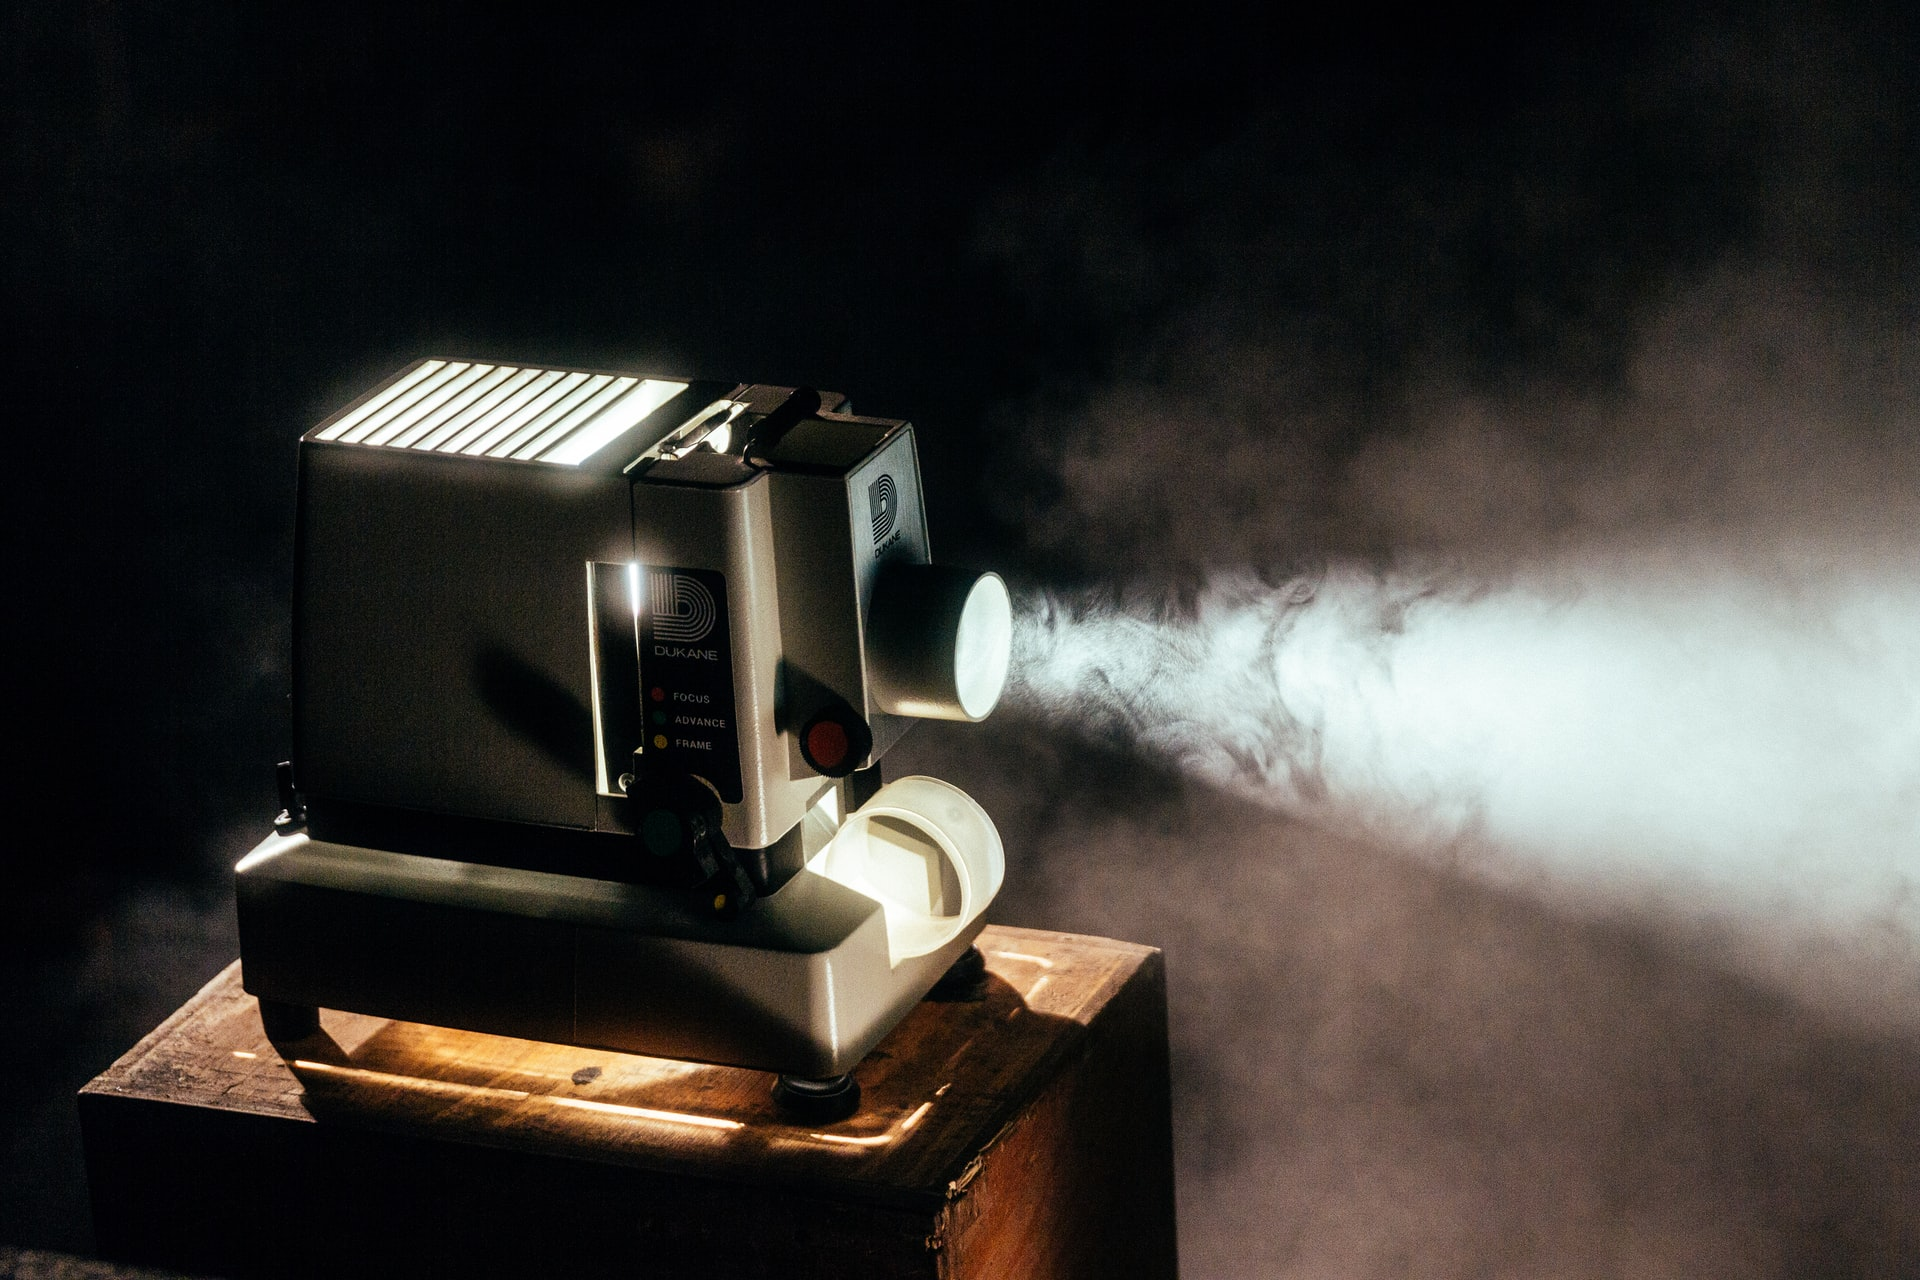
\includegraphics[width=0.8\textwidth]{images/02-projector.jpg}
    \caption{A projector is above all a light emitter. Source: \citet{ImageProjector}}
    \label{fig:background_projector}
\end{figure}

As briefly mentioned in section \ref{section:intro-problem_setting}, no projector is capable of reproducing arbitrary appearance. Each projector can only reproduce a subset of all possible colors, called the \textit{gamut}. Limited projector gamuts have a large impact on how projection mapping is done. To get a better intuition of this impact, we will now explain how a particular type of projector works. We will focus on the so-called Digital Light Processing (DLP) projector which is widely used in cinemas as well as home setups.

\subsubsection{DLP Projectors}
\label{section:background-projection_mapping-projectors-DLP}

Film projectors shine a bright light through film to project its contents onto a screen. But what happens when our movie is digital? What does a DLP projector shine its light through? And what impact does it have on its gamut?

According to \citet{WikiDLP}, DLP projectors project images by filtering the bright white light of their lamp. First, the light goes through a rapidly spinning color wheel which is split into a number of sectors: red, green, blue and sometimes also transparent. At any point, all light from the lamp passes through a single color filter, sending a single-channel image towards the lens. By sending out many single-channel images in rapid succession, however, the projector creates the illusion of sending a three-channel image.

Per-pixel intesities of this single-channel image which form its content are controlled by the Digital Micromirror Device (DMD). This device is divided into many tiny mirrors which roughly correspond to individual pixels of the projected image. Each of these mirrors can either reflect light from the color wheel directly into the lens, or into a heat sink which absorbs it and does not let it through. This allows the projector to turn pixels off and on. Grayscales (pixel intensities between full and zero) are produced by rapidly toggling the mirror between the lens and the heat sink. If, for example, a pixel is on 50\% of the time and off 50\% of the time, the resulting intensity is exactly between full and zero.

\begin{figure}[ht]
    \centering
    \begin{subfigure}[b]{0.49\textwidth}
        \centering
        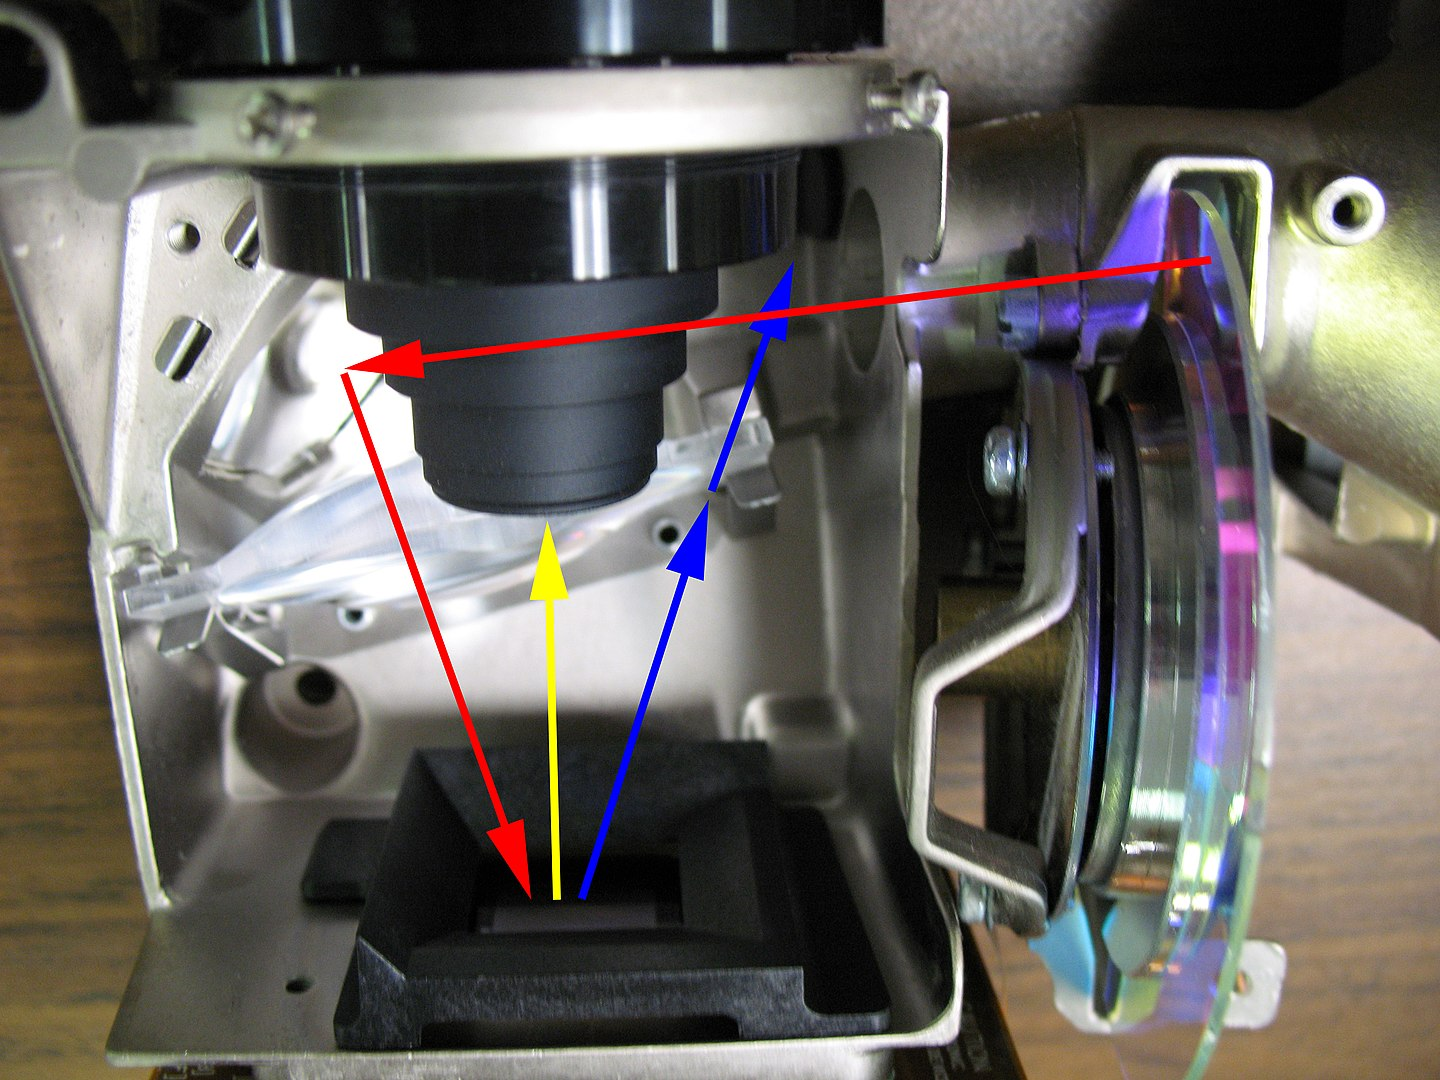
\includegraphics[width=\textwidth]{images/02-projector_dlp.jpg}
        \caption{Source: \citet{ImageProjectorDLP}}
        %\label{}
    \end{subfigure}
    \hfill
    \begin{subfigure}[b]{0.49\textwidth}
        \centering
        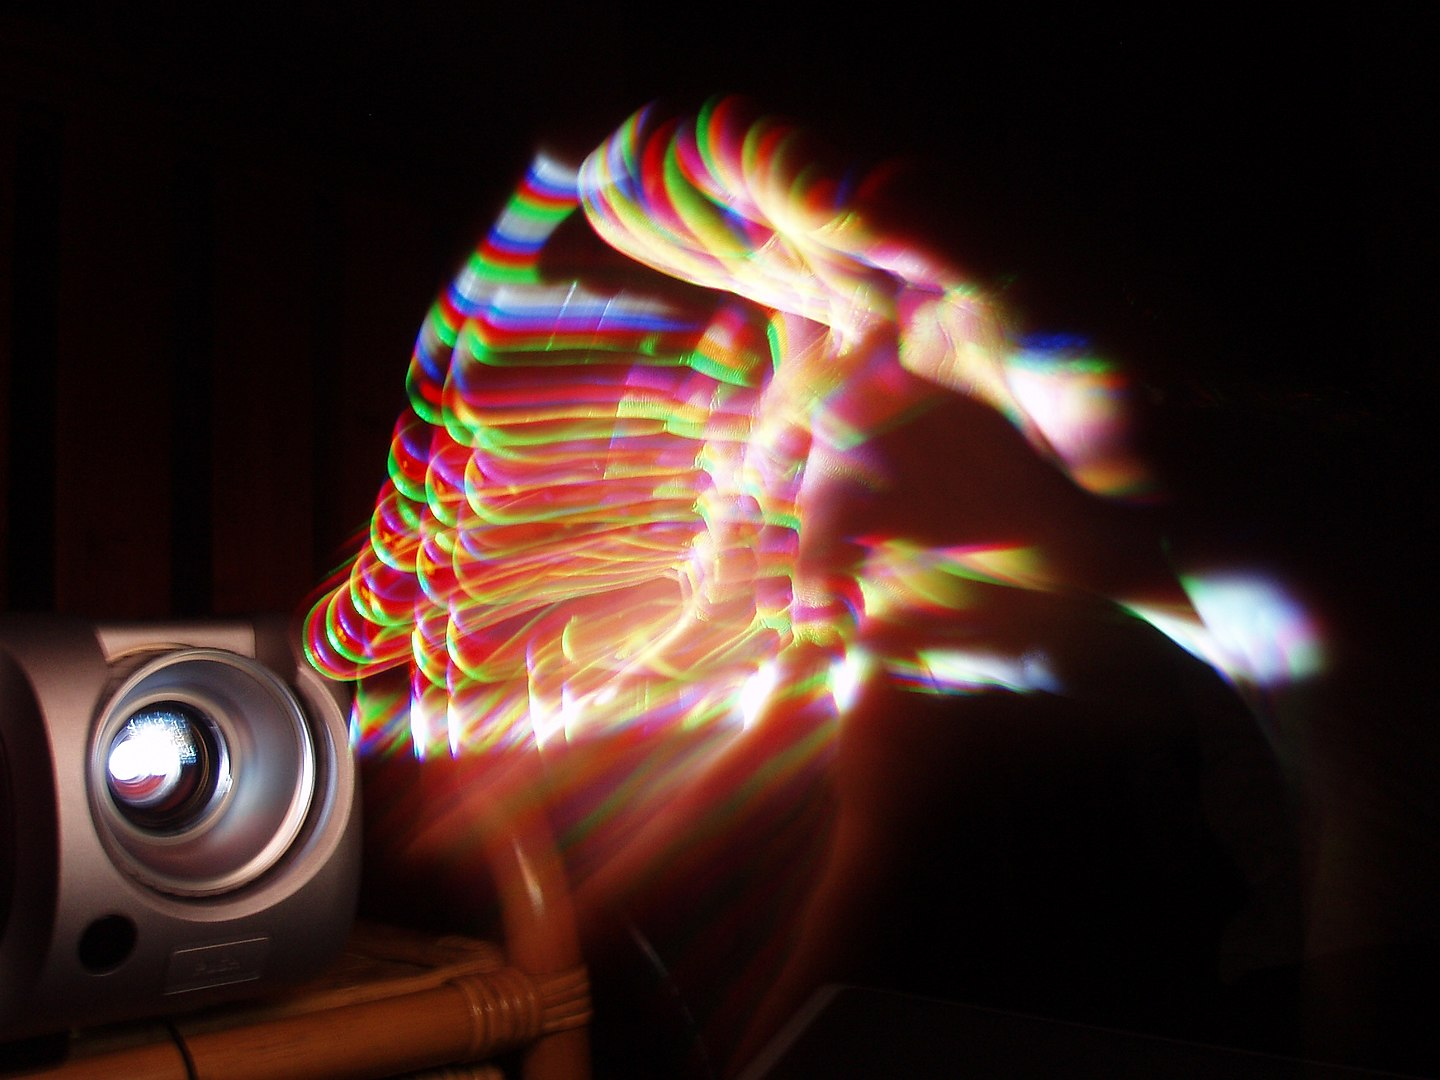
\includegraphics[width=\textwidth]{images/02-projector_rainbow.JPG}
        \caption{Source: \citet{ImageProjectorDLPRainbow}}
        %\label{}
    \end{subfigure}
    \caption{Image a) shows how a DLP projector works. First, bright white light passes through the color wheel. Then it is reflected off the the DMD (red arrows) into either the lens (yellow arrow), or the heat sink (blue arrows). Image b) shows how a DLP projector with a single DMD chip sends out single channel images in rapid succession. This can result in artifacts which can be fixed by using a separate DMD chip for each primary color}
    \label{fig:background_projector_dlp}
\end{figure}

\subsubsection{Gamut Limitations}
\label{section:background-projection_mapping-projectors-limitations}

Based on the way DLPs work, it is easy to see that the process of projecting an image is fairly inefficient since a bright white light is emitted at all times and based on the image being displayed a portion of it is sent into the heat sink and wasted. The main two limitations that result from this and that we are concerned with when projection mapping are limited maximum and minimum brightness.

Maximum brightness is simply limited by the brightness of the lamp. The brighter the lamp, the more energy it consumes and the less efficient it becomes when dark images are being projected.

Minimum brightness is related to the ability of the projector to absorb light which is not reflected directly towards the lens. The more light is absorbed inside the projector, the more the projector heats up. This is why DLP projectors with deep blacks need to be large enough to cool themselves down efficiently. If a DLP projector is not able to absorb all the light, some of it is let through towards the screen and results in dim gray instead of the intended black.

Different projector technologies have different limitations. For example, laser projectors are generally more efficient and brighter because they produce exactly the light color which is needed, as opposed to filtering out white light. But even laser projectors cannot be infinitely bright nor can they subtract light from externally illuminated scenes.

Moreover, even if a particular color lies within the gamut of our projector, the scene that we are projecting onto might prevent us from reproducing that color faithfully. The study of how light interacts with matter to influence what we see around us is called the \textit{light transport theory}. We provide a brief introduction to it in order to understand what our projections look like and which colors are and are not reproducible with a particular scene and projector. But because this theory is rather complex, we begin by building intuition on what to roughly expect when we install a projector and press Play.

{\color{red} TODO: DoF and the thin lens model? (also a limitation that's relevant for us) also pinhole!}

\subsection{Intuition on Projection Appearance}
\label{section:background-projection_mapping-projection_intuition}

The appearance of an object is given by the light it reflects. Light is the visible portion of electromagnetic radiation and consists of photons at various wavelengths. Wavelengths which human vision is sensitive to are approximately between 380 and 780 nm (\citet{PBRT3e}). Shorter wavelengths appear blue, middle ones are green and longer ones are red. Reflectance of an object is defined by the so-called \textit{spectral power distribution} (SPD) which describes what proportion of incoming light is reflected at each wavelength.

\begin{figure}[ht]
    \centering
    \begin{subfigure}[b]{0.49\textwidth}
        \centering
        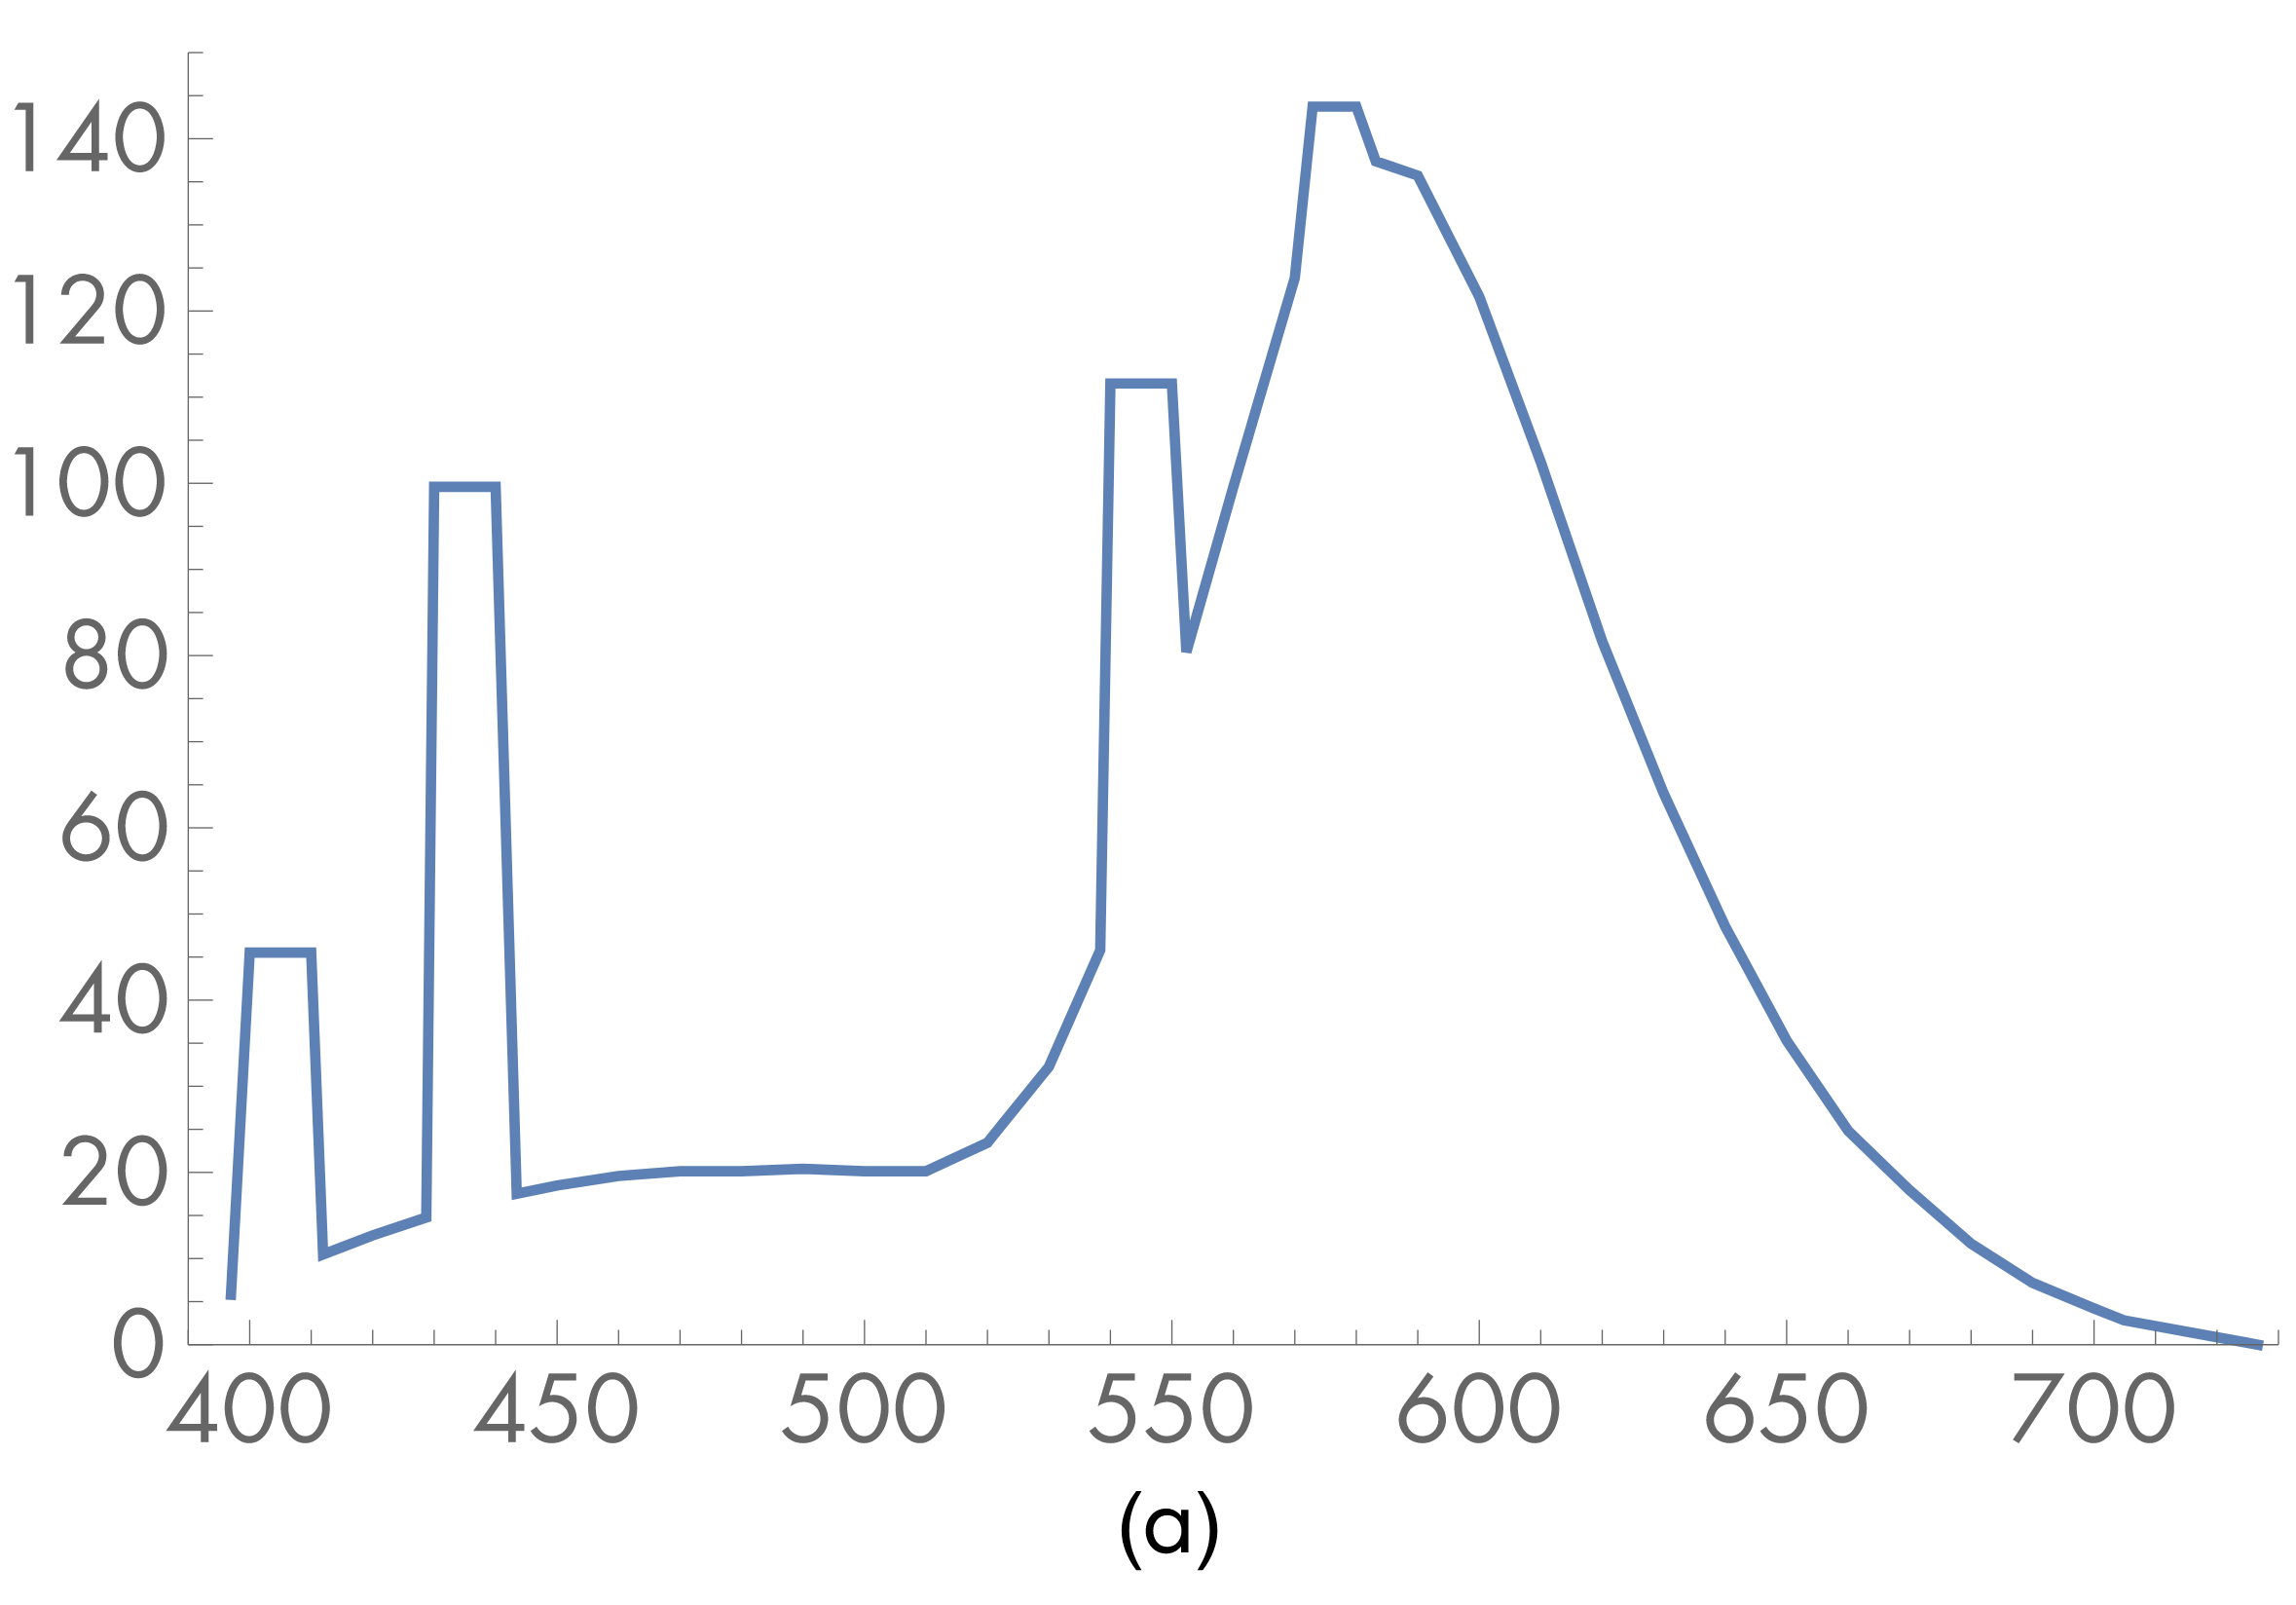
\includegraphics[width=\textwidth]{images/02-spd_fluorescent_light.png}
        \caption*{}
        %\label{}
    \end{subfigure}
    \hfill
    \begin{subfigure}[b]{0.49\textwidth}
        \centering
        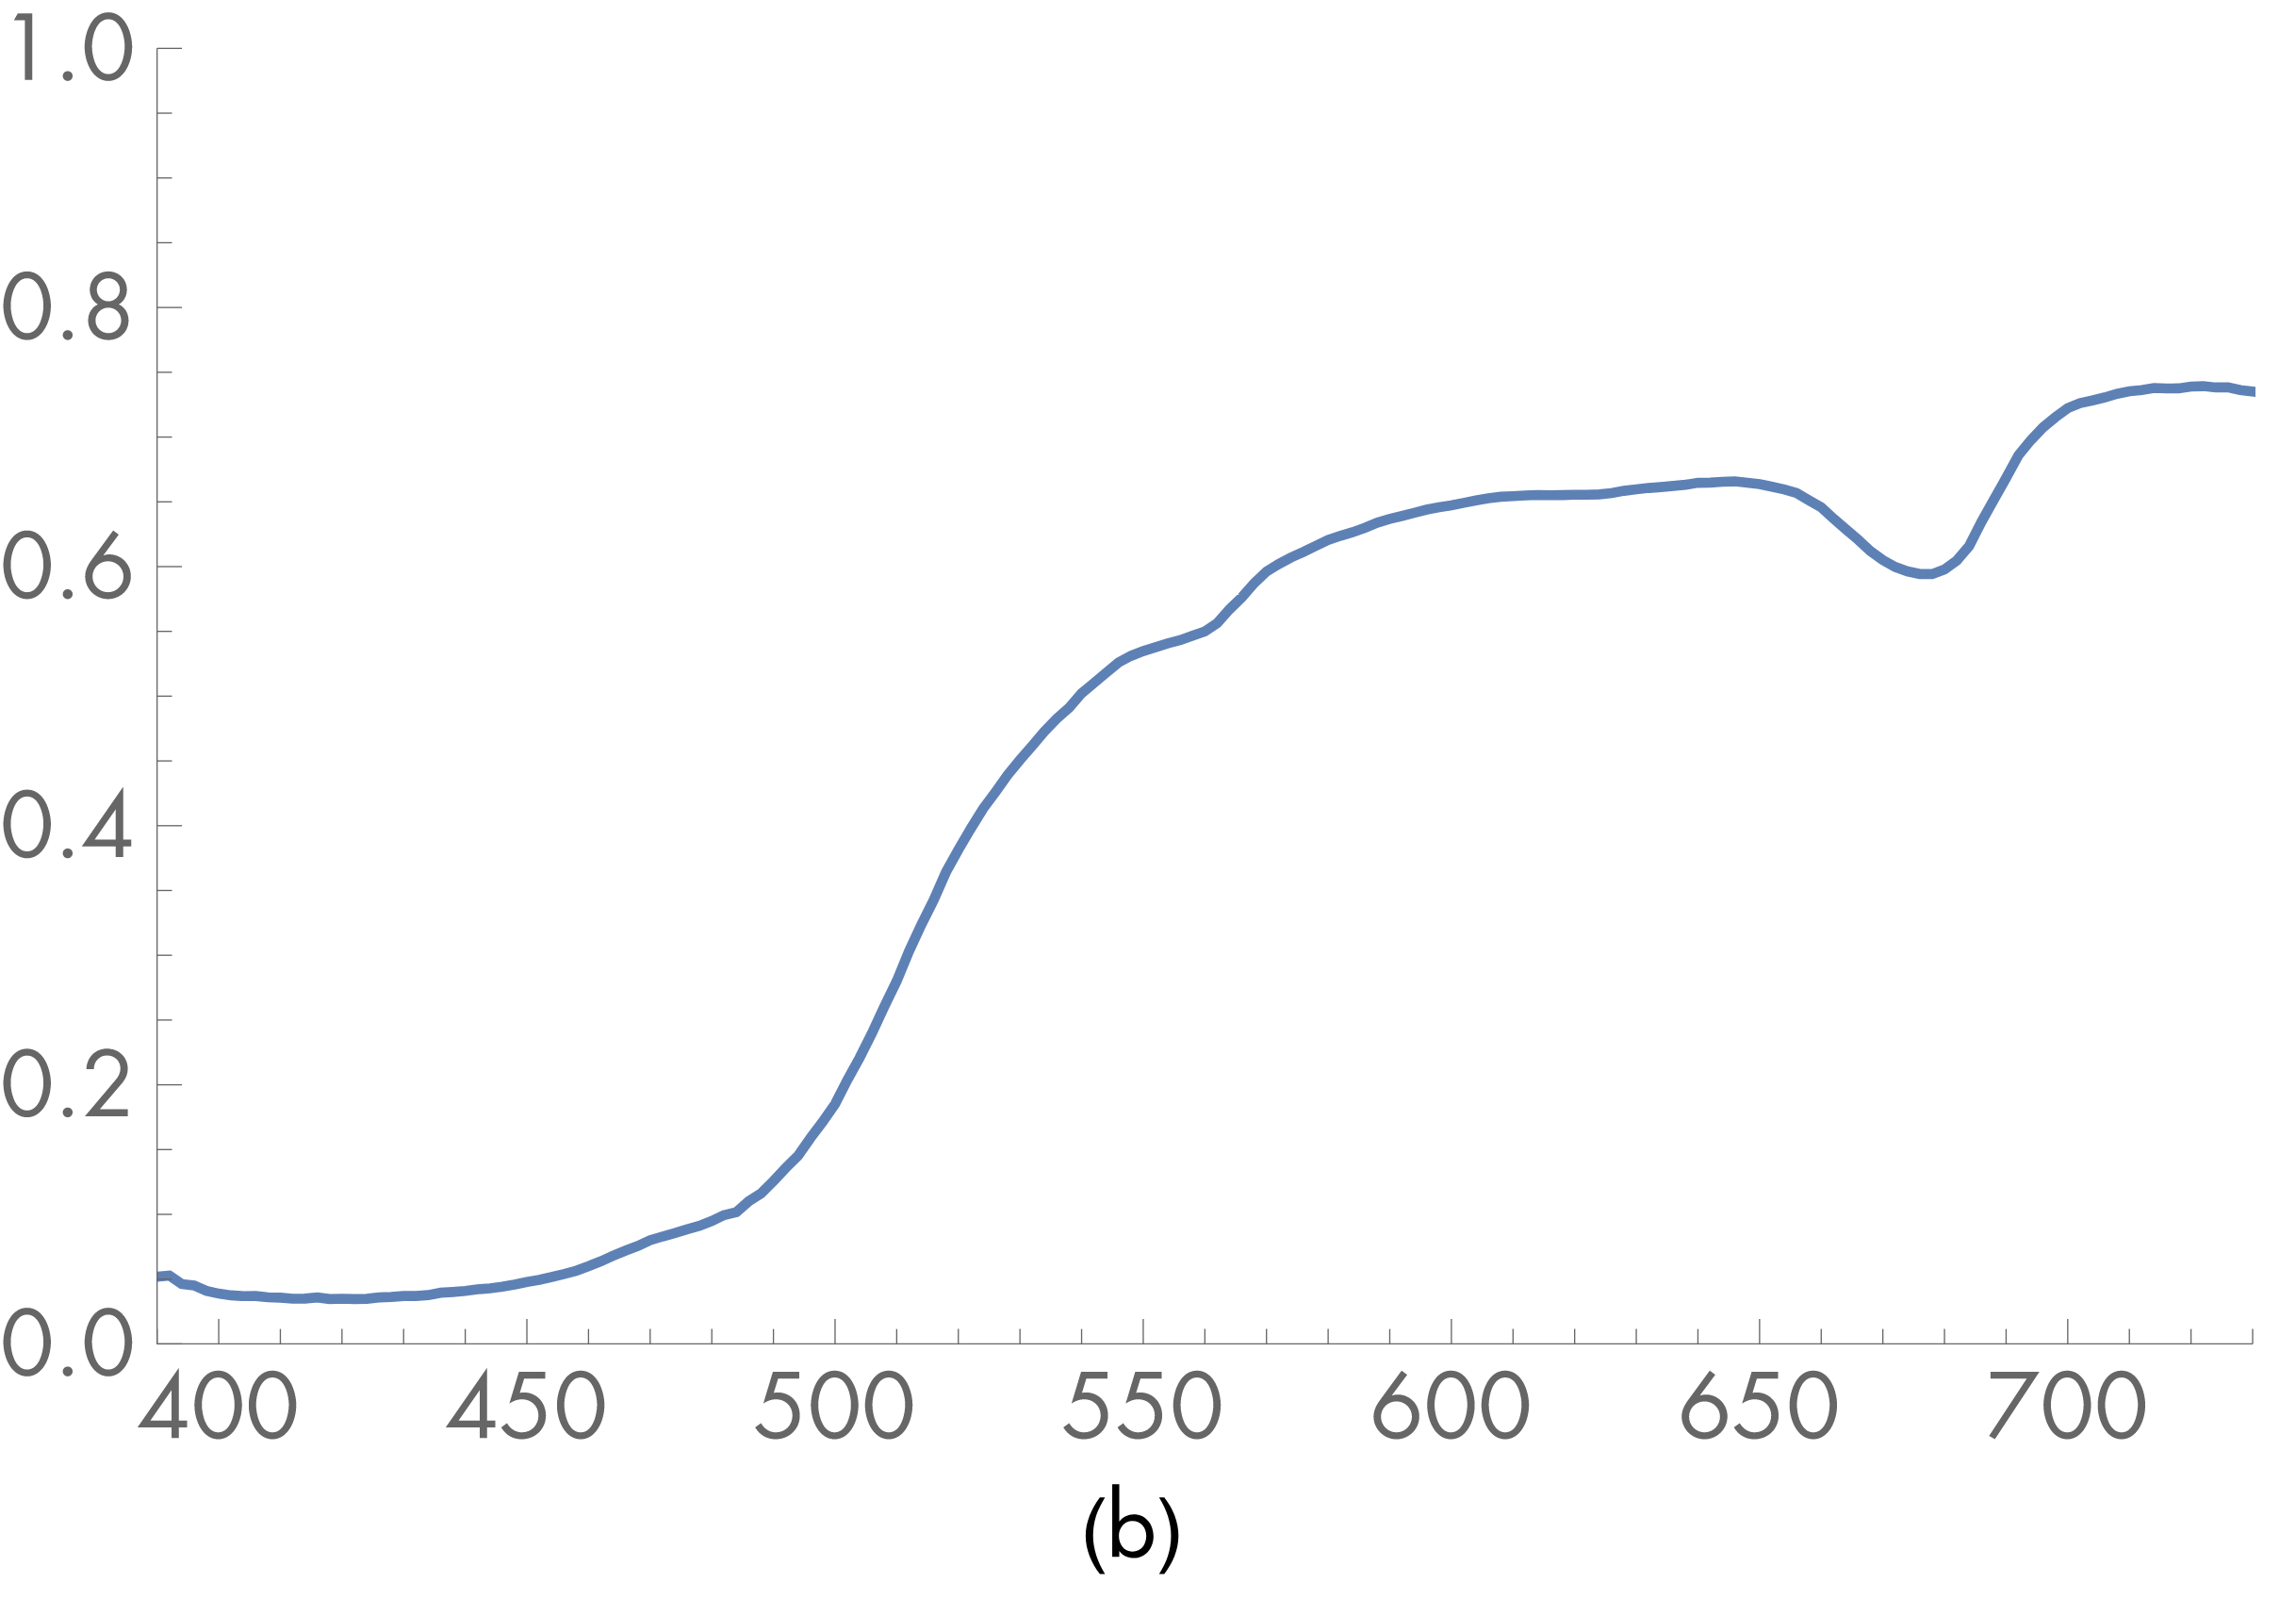
\includegraphics[width=\textwidth]{images/02-spd_lemon_peel.png}
        \caption*{}
        %\label{}
    \end{subfigure}
    \caption{Image a) shows the SPD of fluorescent light with power on the y-axis. Image b) shows the SPD of a lemon peel. Lemon peel is not an emitter hence the y-axis shows the proportion of wavelengths that are reflected off its surface. Source: \citet{PBRT3e}}
    \label{fig:background_spd}
\end{figure}

Projectors are above all light sources. As a matter of fact, each of the millions of tiny mirrors inside the DMD of a DLP projector can be thought of as a separate light source. Projector light has an SPD of its own, describing how much power it carries at each wavelength. When it interacts with a surface, something roughly corresponding to SPD multiplication takes place. If an object does not reflect any light at 450 nm, for example, all of it will be absorbed and will not reach our eyes. See fig. \ref{fig:background_spd_intuition} for examples of how projection interacts with various backgrounds.

\begin{figure}[ht]
    \centering    
    \begin{subfigure}{\textwidth}
        \centering
        \begin{subfigure}{0.24\textwidth}
            \centering
            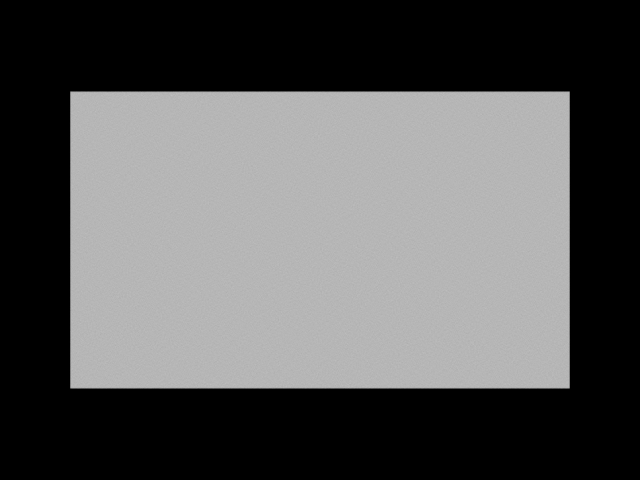
\includegraphics[width=\textwidth]{images/02-spd_intuition-white_white.png}
            \caption*{}
            \label{fig:background_spd_intuition-white_white}
        \end{subfigure}
        \hfill
        \begin{subfigure}{0.24\textwidth}
            \centering
            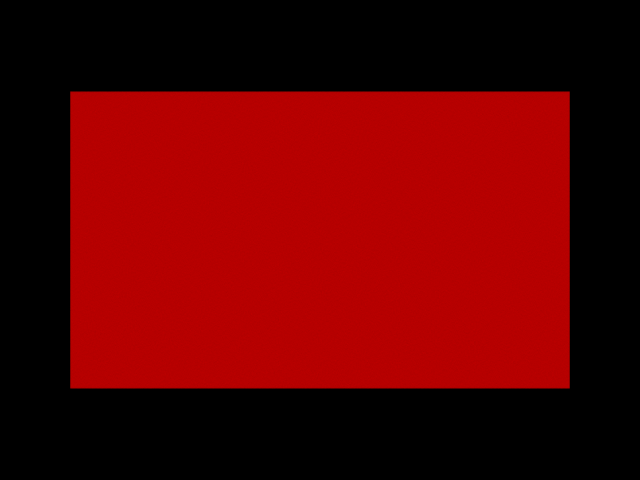
\includegraphics[width=\textwidth]{images/02-spd_intuition-white_red.png}
            \caption*{}
            \label{fig:background_spd_intuition-white_red}
        \end{subfigure}
        \hfill
        \begin{subfigure}{0.24\textwidth}
            \centering
            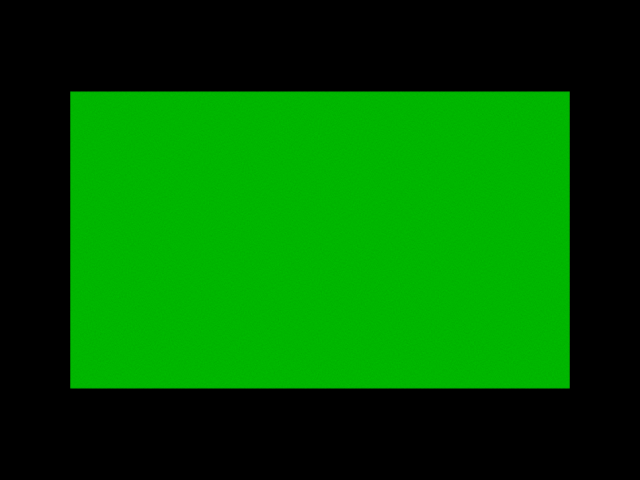
\includegraphics[width=\textwidth]{images/02-spd_intuition-white_green.png}
            \caption*{}
            \label{fig:background_spd_intuition-white_green}
        \end{subfigure}
        \hfill
        \begin{subfigure}{0.24\textwidth}
            \centering
            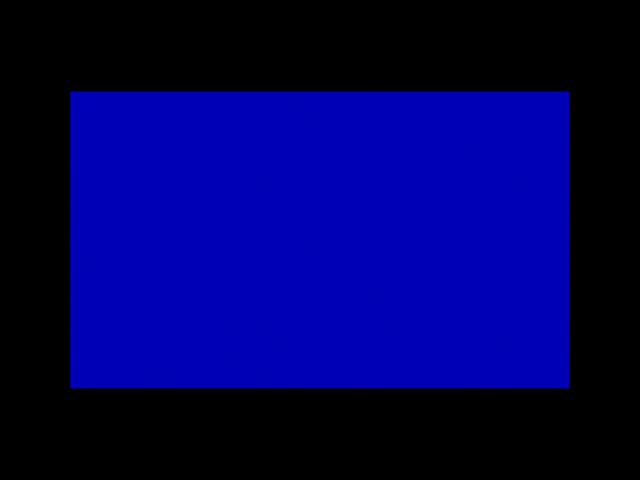
\includegraphics[width=\textwidth]{images/02-spd_intuition-white_blue.png}
            \caption*{}
            \label{fig:background_spd_intuition-white_blue}
        \end{subfigure}
        
        \begin{subfigure}{0.24\textwidth}
            \centering
            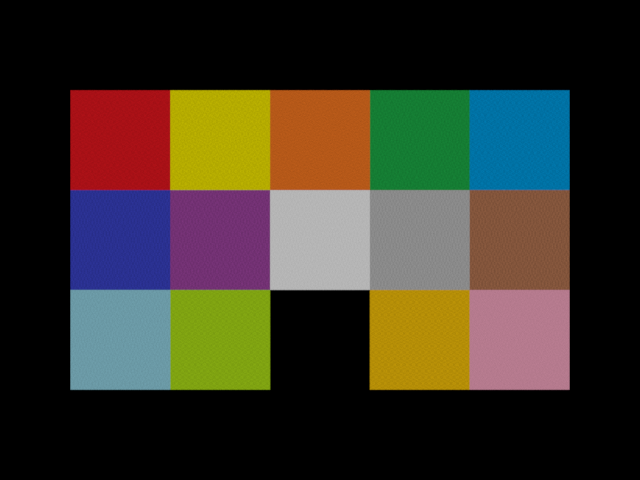
\includegraphics[width=\textwidth]{images/02-spd_intuition-palette_white.png}
            \caption*{}
            \label{fig:background_spd_intuition-palette_white}
        \end{subfigure}
        \hfill
        \begin{subfigure}{0.24\textwidth}
            \centering
            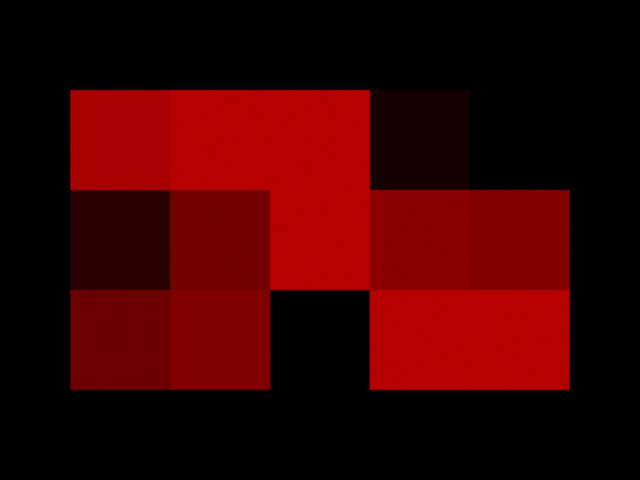
\includegraphics[width=\textwidth]{images/02-spd_intuition-palette_red.png}
            \caption*{}
            \label{fig:background_spd_intuition-palette_red}
        \end{subfigure}
        \hfill
        \begin{subfigure}{0.24\textwidth}
            \centering
            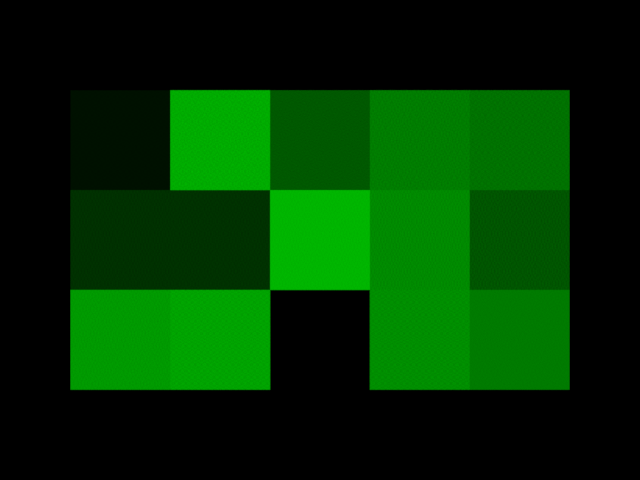
\includegraphics[width=\textwidth]{images/02-spd_intuition-palette_green.png}
            \caption*{}
            \label{fig:background_spd_intuition-palette_green}
        \end{subfigure}
        \hfill
        \begin{subfigure}{0.24\textwidth}
            \centering
            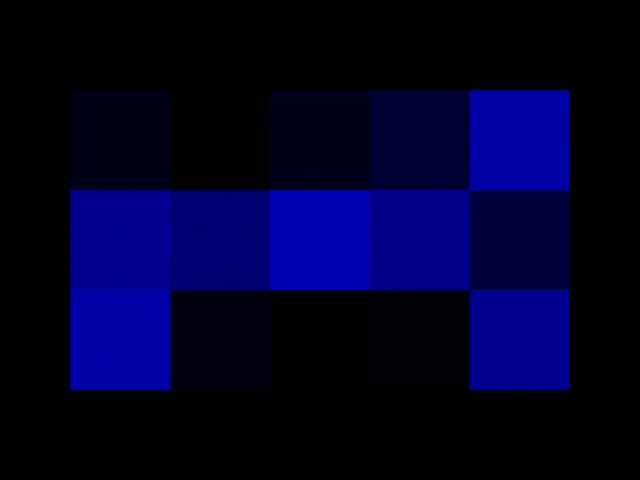
\includegraphics[width=\textwidth]{images/02-spd_intuition-palette_blue.png}
            \caption*{}
            \label{fig:background_spd_intuition-palette_blue}
        \end{subfigure}
    \end{subfigure}
    \caption{In the upper row, white light is projected onto a pure white, red, green and blue wall respectively. In the lower row, a color palette is projected onto the same backgrounds. Note that summing the last three images in each row gives the first one because each background has maximum reflectivity in one color channel and zero reflectivity in others. If a single-chip DLP projector were to project the first image, it would in fact send out the last three in rapid succession.}
    \label{fig:background_spd_intuition}
\end{figure}

We will now study this process more carefully using light transport theory.

\subsection{Light Transport Theory}
\label{section:background-projection_mapping-light_transport}

Light transport theory is the study of how light interacts with matter -- how it travels through space, scatters in fog, reflects from surfaces, refracts in camera lenses and absorbs in black T-shirts in summer. One of the most common uses of light transport is in architectural visualizations (see fig. \ref{fig:background_light_transport_examples-rendering}) and video game and movie rendering. There, we are interested in the SPD that arrives at each pixel of a virtual camera given geometry, materials and light sources.

\begin{figure}[ht]
    \centering
    \begin{subfigure}[b]{0.56\textwidth}
        \centering
        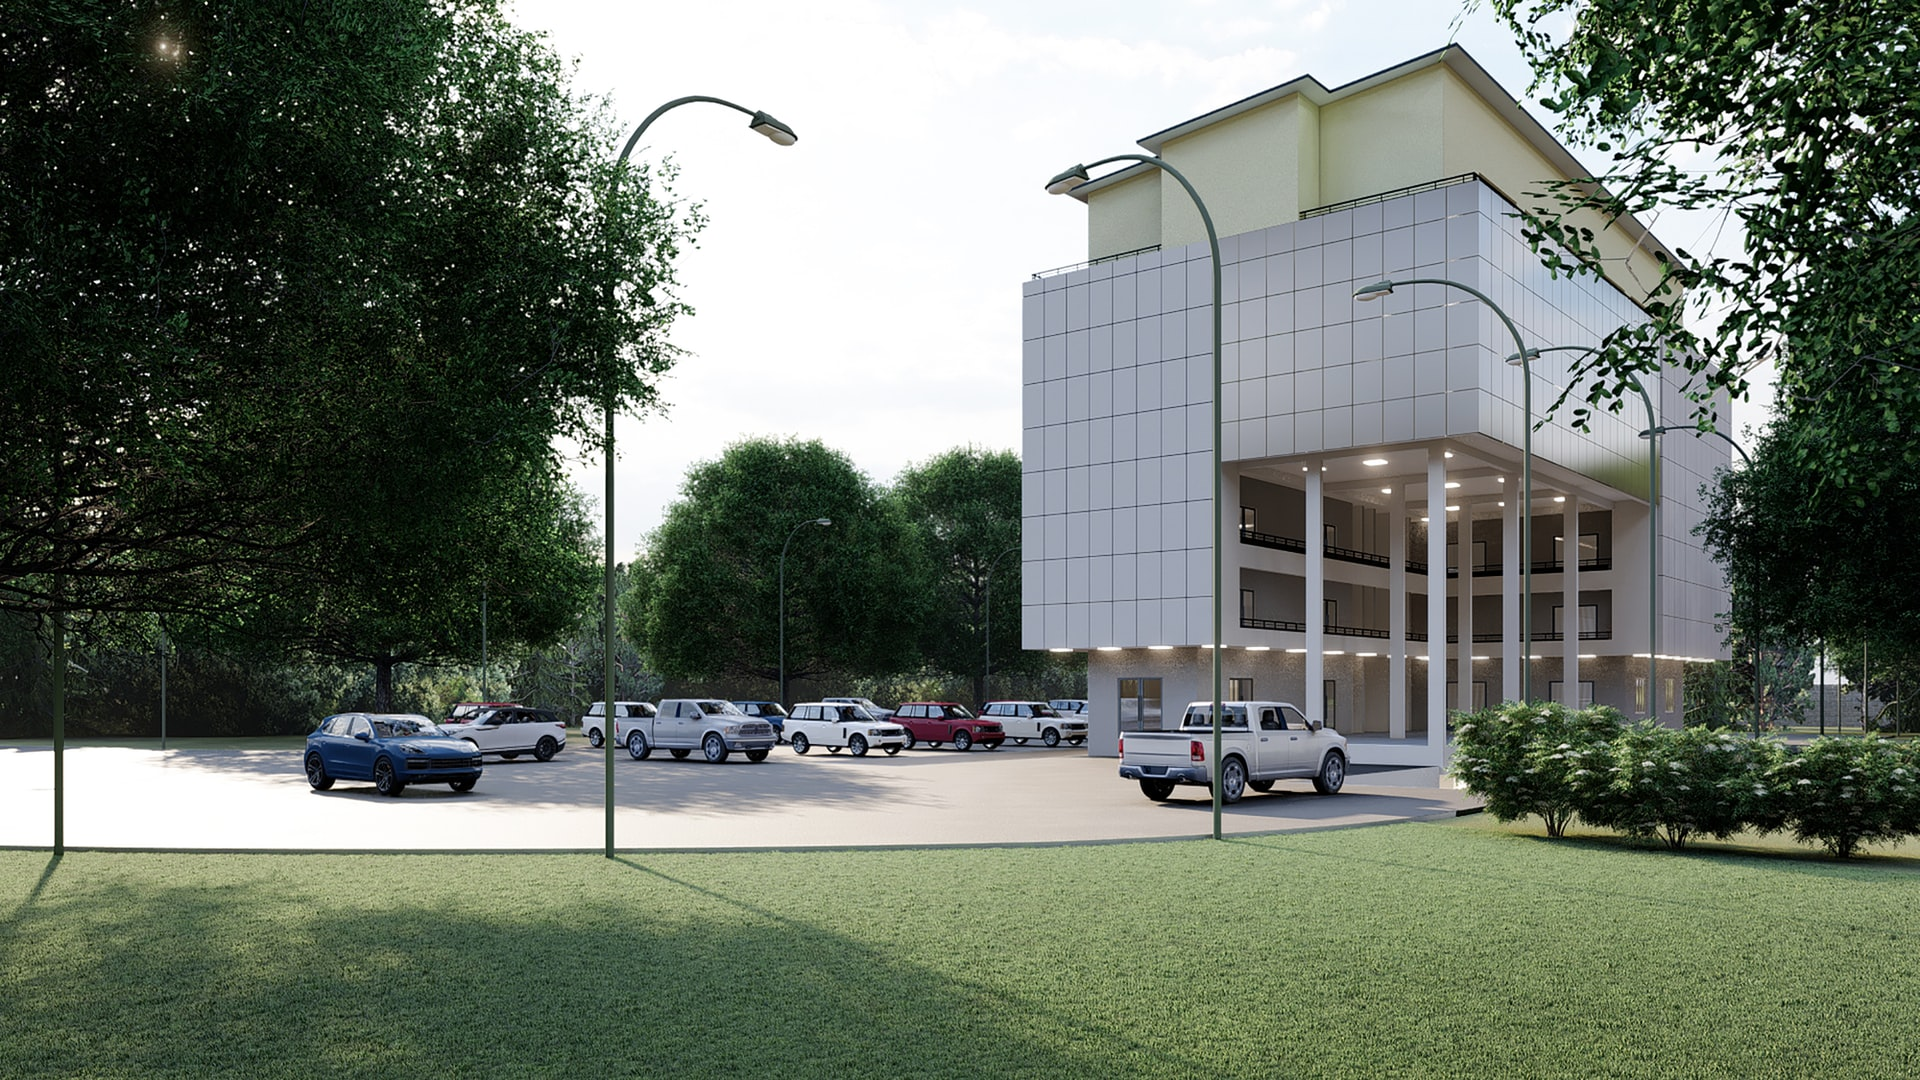
\includegraphics[width=\textwidth]{images/02-rendering.jpg}
        \caption{Source: \citet{ImageRendering}}
        \label{fig:background_light_transport_examples-rendering}
    \end{subfigure}
    \hfill
    \begin{subfigure}[b]{0.42\textwidth}
        \centering
        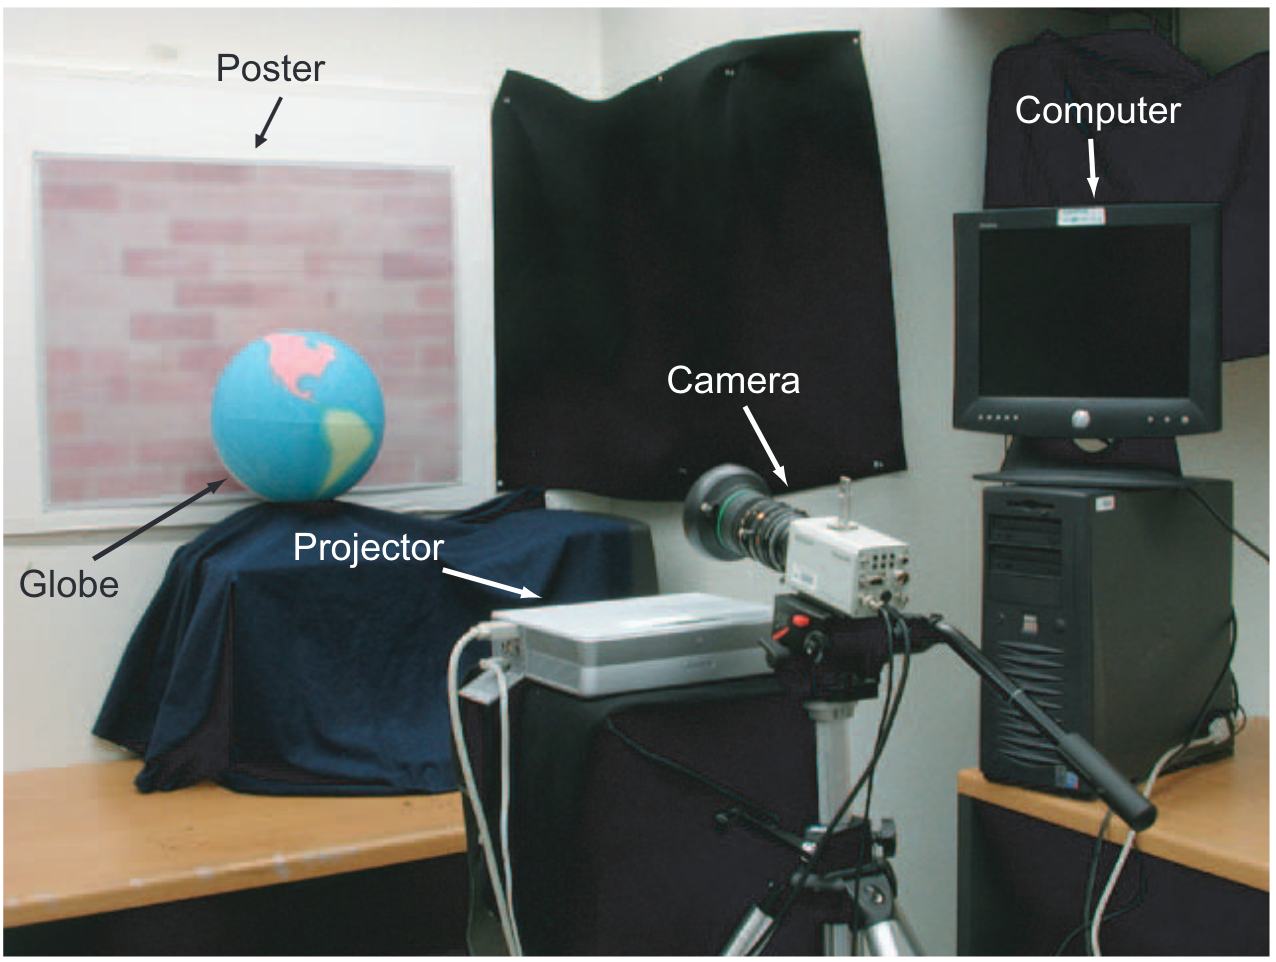
\includegraphics[width=\textwidth]{images/01-procam.png}
        \caption{Source: \citet{Grossberg2004}}
        \label{fig:background_light_transport_examples-procam}
    \end{subfigure}
    \caption{Image a) is an architectural visualization which uses light transport theory to solve the following problem: Given scene geometry, materials and light sources and camera position, what will the camera see? Image b) is a projector-camera system calibration from section \ref{section:intro-problem_setting} and asks: Given what the camera sees when various patterns are projected onto the scene, what can we say about the geometry and materials of the scene?}
    \label{fig:background_light_transport_examples}
\end{figure}

In this section, we provide a brief overview of light transport theory and explain how it can be used in projection mapping. For a more comprehensive coverage, we refer the reader to Physically Based Rendering: From Theory to Implementation by \citet{PBRT3e}.

\subsubsection{Radiance}
\label{section:background-projection_mapping-light_transport-radiance}

As mentioned in \ref{section:background-projection_mapping-projection_intuition}, all we see is light. Measuring light is therefore the crux of understanding how things look. The fundamental quantity we are interested in when measuring light is \textit{radiance}. It is defined as the amount of photons \(Q\) per unit projected area \(A^\perp \) per unit solid angle \(\omega\) per unit of time \(t\) (see fig. \ref{fig:background_radiance}):

\begin{equation}
    \label{eq:radiance}
    L = \frac{dQ}{dA^\perp d\omega dt}
\end{equation}

\begin{figure}[ht]
    \centering
    \def\svgwidth{0.8\textwidth}
    \input{images/figures/02-radiance.pdf_tex}
    \caption{Illustration of radiance which is defined as the amount of photons \(Q\) per unit projected area \(A^\perp \) per unit solid angle \(\omega\) per unit of time \(t\)}
    \label{fig:background_radiance}
\end{figure}

As suggested in fig. \ref{fig:background_spd}, to see the full picture, we need to consider radiance at each visible wavelength. A common approach to simplifying this is decompose the space of all visible SPDs into three basis functions which roughly correspond to red, green and blue colors. In that case, we would be interested in radiance in each of these channels. To simplify our explanations even further, we only talk about radiance \(L\). It is, however, important to realize that there is a layer of complexity hidden behing that notation.

Another issue with radiance is that it is a purely physical quantity while how we perceive something is to do with psychology. Luckily, for each radiometric measurement, such as radiance, there is a corresponding \(photometric\) measurement which expresses how a stimulus is perceived by the human visual system. The photometric counterpart to radiance is \(luminance\) and can be obtained from radiance by integrating against an empirically constructed spectral response curve which describes how the human eye reacts to various wavelengths. Because luminance can be easily computed from radiance, we only discuss radiance in this thesis.

We will now present the relationship between objects, light sources and the radiance incoming onto our camera sensor or eye retina. This relationship sits at the heart of light transport theory and is called the \textit{rendering equation}.

\subsubsection{Rendering Equation}
\label{section:background-projection_mapping-light_transport-rendering_equation}

The rendering equation describes the amount of outgoing radiance from point \(x\) in a scene towards a direction \(\mathbf{v}\):

\begin{equation}
    \label{eq:rendering_equation}
    L(x \rightarrow \mathbf{v}) = \int_{\Omega(x)} L(x \leftarrow \mathbf{u}) f_r(x, \mathbf{u} \rightarrow \mathbf{v}) \cos \theta d\mathbf{u} + E(x \rightarrow \mathbf{v})
\end{equation}

{\color{red} TODO: figure of rendering equation}

where \(L(x \leftarrow \mathbf{u})\) is the radiance arriving at \(x\) from direction \(\mathbf{u}\), \(\Omega(x)\) is the hemisphere oriented to the direction of the surface normal at \(x\), \(f_r\) is the spatially-varying bidirectional reflectance distribution function (SVBRDF) which determines surface reflectance for each point \(x\), incoming direction \(\mathbf{u}\) and outgoing direction \(\mathbf{v}\), and \(\theta\) is the angle between \(u\) and the surface normal at \(x\). Finally, \(E(x \rightarrow \mathbf{v})\) is the radiance emitted from \(x\) towards \(\mathbf{v}\) in case \(x\) lies on a light source.

The main idea of the equation is that radiance leaving towards \(\mathbf{v}\) from \(x\) is the sum of reflected and emitted radiance. It assumes empty space between objects, therefore no light scattering occurs between them. This means that radiance is constant along straight lines and the equation is recursive -- \(L(x \leftarrow \mathbf{u}) = L(y \rightarrow -\mathbf{u})\) where \(y\) is the point seen from \(x\) in the direction of \(\mathbf{u}\). Generalizations of the rendering equation to scenes with participating media where this is not the case are discussed in a SIGGRAPH course by \citet{Novak2018}.

Apart from assuming that our objects are in vacuum, the equation also assumes that light is reflected from the same point it arrived at. This is generally not the case as can be seen for example with human skin where light bounces under the surface before it is reflected. This phenomenon is known as \textit{subsurface scattering} and a generalization of the rendering equation to account for it has been presented for example by \citet{Jensen2001}. For our purposes, however, it is sufficient to be familiar with the basic form of the rendering equation.

To determine the amount of radiance that hits a virtual camera sensor in scenes such as fig. \ref{fig:background_light_transport_examples-rendering}, we need to solve the rendering equation for points that lie on the sensor and directions towards points in the scene that are visible from the sensor. This is typically done by Monte Carlo integration which estimates the integral by random sampling. Each sample is a light path from a light source towards the camera with zero or more bounces on the surfaces of the scene. A strategy to choose such samples is crucial to the performance of a rendering algorithm. A brilliant overview of sampling strategies, for example bidirectional path tracing (BDPT) can be found in \citet{Veach1997}.

\subsubsection{Towards Projection Mapping}
\label{section:background-projection_mapping-light_transport-towards_projection_mapping}

In a sense, projection mapping is a more difficult problem than rendering. Whereas in rendering, the scene geometry, materials and light sources are known and the radiance at the camera sensor is unknown, in projection mapping we only know the radiance at the camera sensor and everything else, including the projection image (our light source), is unknown.

{\color{red} TODO: figure that compares rendering to projection mapping}

Projection mapping algorithms therefore do not typically solve the full (inverse) light transport of the whole scene, but instead they build on top of assumptions and provide estimates. Common assumptions are for example

\begin{itemize}
    \item A known relationship between the projector and camera orientation
    \item Absence of glossy surfaces whose appearance depends on view point
    \item A 1:1 correspondence between projector and camera pixels, meaning that each pixel of the camera image is influenced by only one projector pixel. Note that this does not hold for example in scenes with convex geometry where light from multiple projector pixels is concentrated into a single camera pixel
\end{itemize}

We will now review some common approaches to projection mapping found in state-of-the-art methods. Our goal is to use this information to construct a reference method that we can implement in our projector-camera system simulator and use in experiments to compare our proposed projection mapping method against.

\subsection{Projector-Camera Systems}
\label{section:background-projection_mapping-procams}

The key idea in projection mapping is to use a camera to observe the projection and provide information on how to adapt it to achieve desired appearance. This system as a whole is called the \textit{projector-camera system}, commonly shortened as \textit{procam}.

As mentioned in eq. \ref{eq:projection_mapping-per_pixel}, this adaptation is done by modifying the projector image until the camera image matches the desired appearance pixel by pixel. However, the relationship between projector and camera pixels is very complex, as suggested in section \ref{section:background-projection_mapping-light_transport} on light transport theory. The model of this relationship is the main differentiating factor of various projection mapping methods.

On a high level, projection mapping methods can be split into two groups:

\begin{itemize}
    \item Those that assume a 1:1 correspondence between projector and camera pixels
    \item Those that do not and instead attempt to solve general light transport in the whole scene
\end{itemize}

The first group usually has two smaller tasks to perform. First, they need to establish those correspondencies geometrically in a step called \textit{geometric calibration}. Then, they need to model how the intensity of a projector pixel affects the intensity of the corresponding camera pixel in a step called \textit{radiometric calibration}. Despite the original assumption of 1:1 pixel correspondence, these methods are reasonably general and work quite well. They are also the most common. We will therefore review a few of them and focus on how projector hardware (along with scene complexity) limits their performance.

The second group typically uses \textit{inverse light transport} to model the relationship between projector and camera as generally as possible. These methods are mostly limited by the computational complexity of such a task. Some, for example \citet{Siegl2017}, achieve real time performance at the cost of using an additional depth camera to gain more information about the scene and projecting only on matte objects of constant color. We will focus on an older method by \citet{Wetzstein2007} that works with arbitrarily complex scenes and will thus be useful for us when constructing our reference method.

For a complete overview of the state of the art in projection mapping, see \citet{Grundhofer2018}.

\subsubsection{Geometric Calibration}
\label{section:background-projection_mapping-procams-geometric_calibration}

The goal of geometric calibration is to find a point \(M_c = [u_c, v_c]^T\) in the camera image for each point \(M_p = [u_p, v_p]^T\) in the projector image such that the value of the latter determines the value of the former. These correspondencies are usually established via a third point, \(P = [x, y, z]\) which is located in the scene.

The relationship between \(M_c\) and \(P\) is determined by the \textit{intrinsic} and \textit{extrinsic} matrices:

\begin{equation}
    \label{eq:camera_equation}
    \begin{bmatrix}
        u_c \\
        v_c \\
        1
    \end{bmatrix} =
    \begin{bmatrix}
        f_x & s & u \\
        0 & f_y & v \\
        0 & 0 & 1 
    \end{bmatrix} \cdot
    \begin{bmatrix}
        \mathbf{R} & \mathbf{t}
    \end{bmatrix} \cdot
    \begin{bmatrix}
        x \\
        y \\
        z
    \end{bmatrix}
\end{equation}

where the intrinsic matrix is formed by camera focal lengths \(f_x\) and \(f_y\) (focal length is expressed in pixels and if pixels are square, then \(f_x = f_y = f\)), skewness \(s\) of image axes, and principal point coordinates \([u, v]^T\) (the intersection of optical axis and image plane which is generally not in the center of the image). The extrinsic matrix is then formed by rotation \(\mathbf{R}\) and translation \(\mathbf{t}\) which convert between world coordinates and camera coordinates. See fig. \ref{fig:background_camera_calibration} for an illustration.

\begin{figure}[ht]
    \centering
    \def\svgwidth{0.8\textwidth}
    \input{images/figures/02-camera_calibration.pdf_tex}
    \caption{Illustration of geometric calibration of projector and camera. Points \(M_c\) and \(M_p\) on camera and projector image plane, respectively, are related via a point \(P\) in the scene. \(f\) is the focal length which is the distance between pinhole and principle point and \(u\) and \(v\) are principle point coordinates with respect to image plane origin}
    \label{fig:background_camera_calibration}
\end{figure}

The most commonly used method for finding the parameters of eq. \ref{eq:camera_equation} was introduced by \citet{Zhang1999}. They are estimated by taking at least two photos of a planar pattern at various orientations.

We will now outline two recent methods to perform geometric calibration. The first one requires user assistance, while the second one is fully automatic.

\textbf{One camera, one projector and a calibration board.} The first method, introduced by \citet{Yang2016}, uses a calibration board containing a random dot pattern. First, the camera is calibrated using the approach of \citet{Zhang1999}. Then the projector is calibrated by projecting another dot pattern onto the board and treating the projector as an inverse camera. The whole process needs around 10 views of the calibration board according to experiments in the paper.

\textbf{Two cameras, one projector.} An entirely automatic self-calibration method was presented by \citet{Willi2017}. Their method first establishes pixel correspondencies between the two cameras and then continues to estimate the intrinsic and extrinsic matrix, as well as the 3D point cloud of the scene. Finally, the projector is calibrated using this information. It is worth noting that this method works also for any larger number of projectors and cameras in which case camera pairs are sorted by the quality of their pixel correspondencies. Calibration is first done for the best pair and other devices are incorporated iteratively, improving the overall estimate.

\subsubsection{Radiometric Calibration}
\label{section:background-projection_mapping-procams-radiometric_calibration}

Once correspondencies between projector and camera pixels have been established, radiometric calibration can be performed. In general, the goal is to find a color-mapping function \(f\) such that

\begin{equation}
    \label{eq:radiometric_calibration}
    \begin{bmatrix}
        C_R \\
        C_G \\
        C_B
    \end{bmatrix} = f(
        \begin{bmatrix}
            P_R \\
            P_G \\
            P_B
        \end{bmatrix}
    )
\end{equation}

where \(C\) is the color of a camera pixel and \(P\) is the color of the corresponding projector pixel. We describe one method that assumes \(f\) to be linear and one method that allows for arbitrary \(f\).

\textbf{Linear color-mapping function.} One of the first projection mapping methods was presented by \citet{Grossberg2004}. There, the relationship between \(c_c\) and \(c_p\) is specified as follows:

\begin{equation}
    \label{eq:linear_color_mapping}
    \begin{bmatrix}
        C_R \\
        C_G \\
        C_B
    \end{bmatrix} = p_c(
        \begin{bmatrix}
            V_{RR} & V_{RG} & V_{RB} \\
            V_{GR} & V_{GG} & V_{GB} \\
            V_{BR} & V_{BG} & V_{BB}
        \end{bmatrix} \cdot p_p(
            \begin{bmatrix}
                P_R \\
                P_G \\
                P_B
            \end{bmatrix}
        ) +
        \begin{bmatrix}
            F_R \\
            F_G \\
            F_B
        \end{bmatrix}
    )
\end{equation}

where \(p_p\) is a non-linear projector response function which turns input pixel values into projector brightness, \(p_c\) is a non-linear camera response that converts radiance arriving at the camera sensor to output pixel value, \(F = [F_R, F_G, F_B]^T\) is the environment light term which is independent of the projector, and finally \(V\) is a \(3 \times 3\) color mixing matrix which captures the relationship between projector and camera channels and their interactions with spectral reflectance.

Both \(p_p\) and \(p_c\) are independent of the scene and can be estimated separately. \(V\) and \(F\) are per-pixel and scene-dependent and can be estimated by projecting and capturing 6 calibration images.

The disadvantage of this method is that the linear color mixing matrix is not an accurate model for example when using DLP projectors described in section \ref{section:background-projection_mapping-projectors-DLP}. DLP projectors sometimes form an image by composing red, green, blue and white channels together. The extra white channel may result in non-linear behavior. Another disadvantage is related to projector brightness limitations. If the color gamut of the projector struggles to reproduce the color required by the compensation model, it results in clipping artifacts and lowered contrast. See fig. \ref{fig:background_clipping} for an illustration.

\begin{figure}[ht]
    \centering
    \def\svgwidth{0.6\textwidth}
    \input{images/figures/02-clipping.pdf_tex}
    \caption{Illustration of reduced contrast due to brightness limitations. Projector gamut is delimited by a triangle. If a compensation model requires a color which is outside the triangle, the closes color on the edge of the triangle is projected instead. Colors inside the triangle are projected as required which results in reduced contrast between the two groups}
    \label{fig:background_clipping}
\end{figure}

\textbf{Non-linear color-mapping function with a global optimization step.} To solve these problems, \citet{Grundhofer2015} presented an improved method which allows for an arbitrary color-mixing function. This function is estimated by obtaining up to \(6^3\) samples and then applying thin-plate spline interpolation on them. This sampling process takes several minutes but once it is completed, compensation can be performed in real time.

Moreover, the paper acknowledges that the contrast issues stem from the way the camera image is matched with the desired appearance pixel by pixel (see eq. \ref{eq:projection_mapping-per_pixel}). To fix this, it uses a global optimization step which compensates the image based on its higher level content. In this step, a patch size is chosen (typically \(2^n\) pixels) and a color-correcting coefficient is introduced for each patch. The coefficients are set so as to minimize clipping errors caused by limited color gamut of the projector and overall increase image contrast.

\begin{figure}[ht]
    \centering
    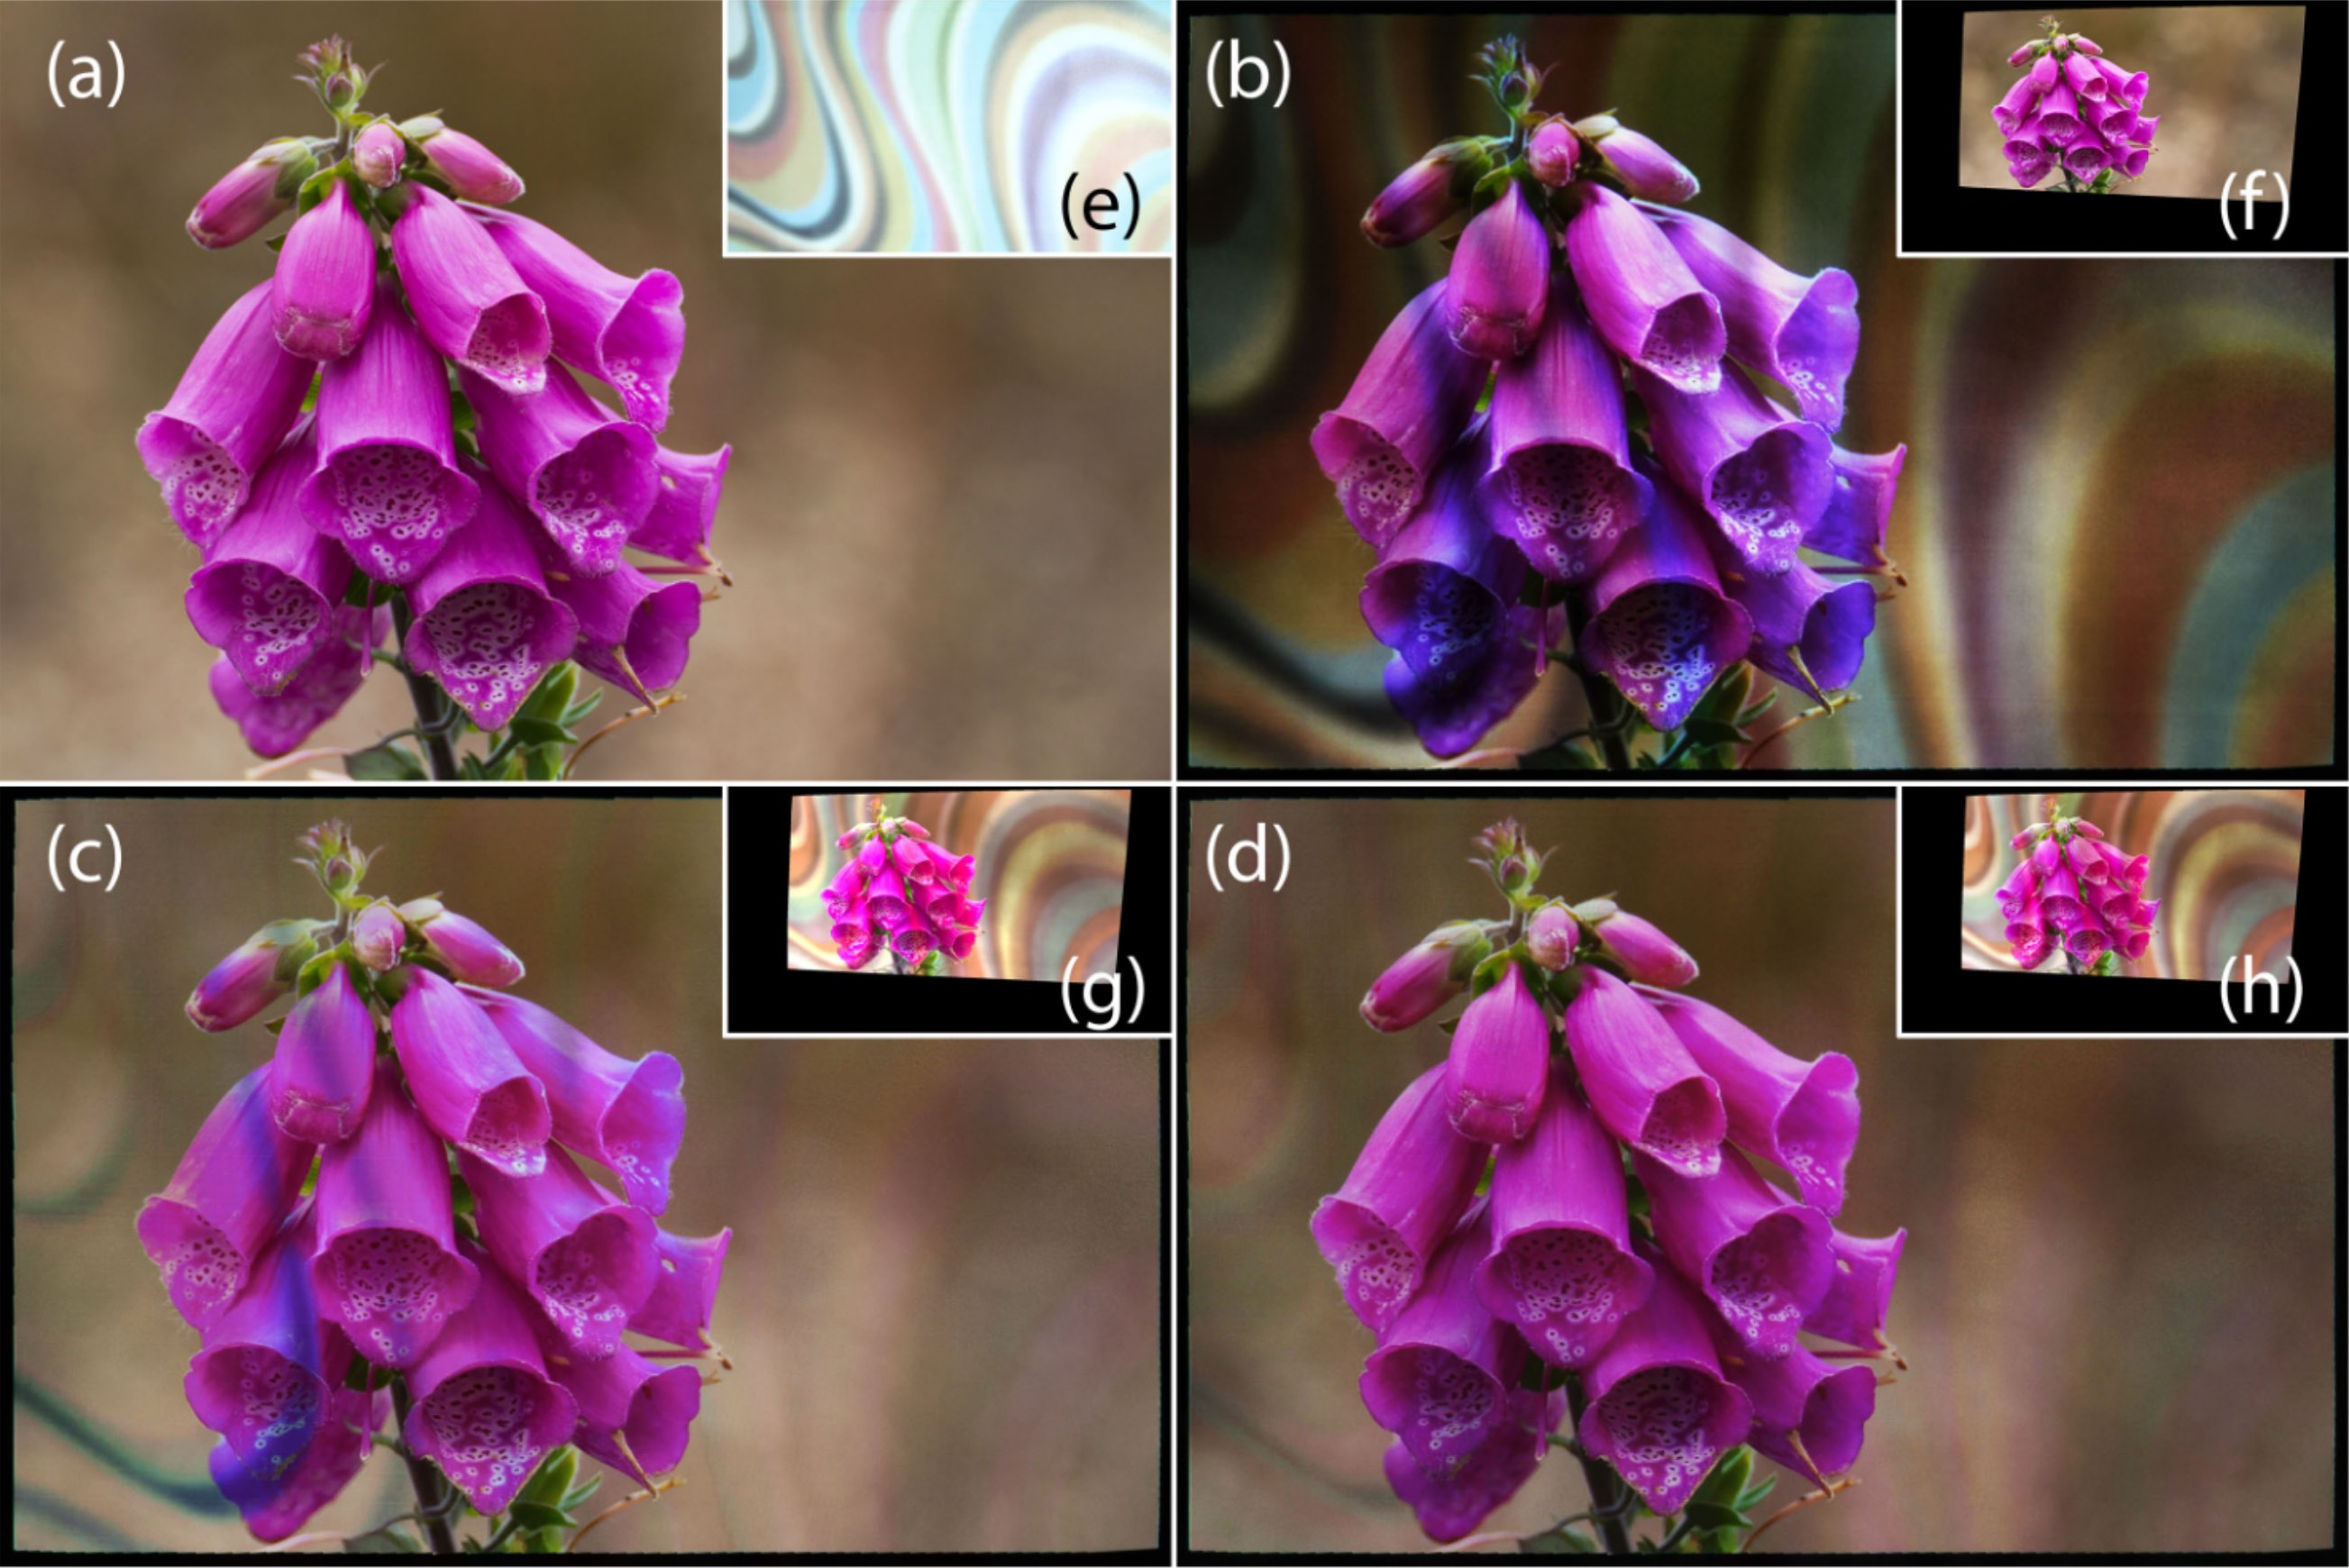
\includegraphics[width=0.6\textwidth]{images/02-grundhofer_result_compressed.jpg}
    \caption{Results of a projection mapping method by \citet{Grundhofer2015}. (a) original input image. (e) non-uniformly colored projection surface (illuminated  uniformly white). (b) captured projection of (a) on (e). (c) captured  projected  compensation  image shows local clipping errors. (d) reduced clipping errors after applying a global optimization step. (f-h) geometrically warped projection images generating camera images (b-d). Source: \citet{Grundhofer2015}}
    \label{fig:background_grundhofer_result}
\end{figure}

As a result, this method achieves very good results in scenes which have minimal inter-reflection that cannot be modeled when 1:1 correspondence between projector and camera pixels is assumed (see fig. \ref{fig:background_grundhofer_result}). The idea of the global optimization step is important because goes in the same direction as our method -- compensating the projection image not pixel by pixel, but based on higher-level content instead.

\subsubsection{Inverse Light Transport}
\label{section:background-projection_mapping-procams-inverse_lt}

Another approach to projection mapping that does not rely on the assumption of 1:1 correspondence between projector and camera pixels is so-called inverse light transport. The basic idea behind this approach is that radiance incoming onto camera sensor is a linear function of light sources in the scene. This can be derived directly from the rendering equation (see eq. \ref{eq:rendering_equation}) and practical examples can be seen in fig. \ref{fig:background_linear_lt}.

\begin{figure}[ht]
    \centering
    \begin{subfigure}[b]{0.24\textwidth}
        \centering
        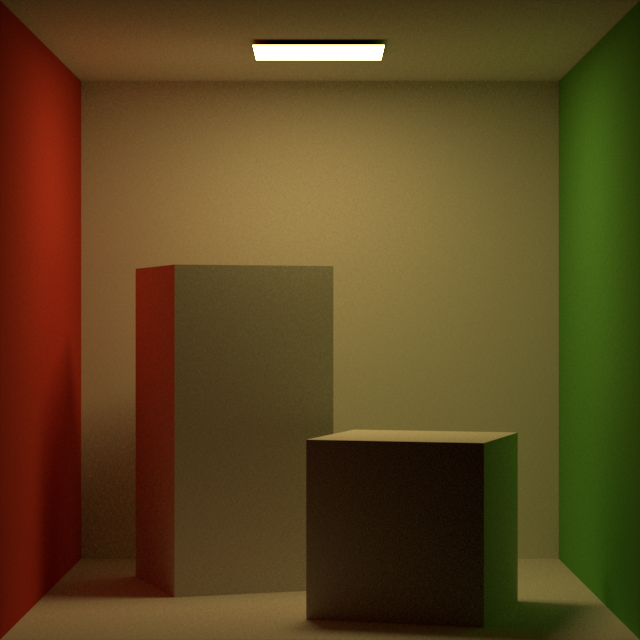
\includegraphics[width=\textwidth]{images/02-linear_lt_light01.jpg}
        \caption*{\(a = 1.0\), \(b = 0.0\)}
        %\label{}
    \end{subfigure}
    \hfill
    \begin{subfigure}[b]{0.24\textwidth}
        \centering
        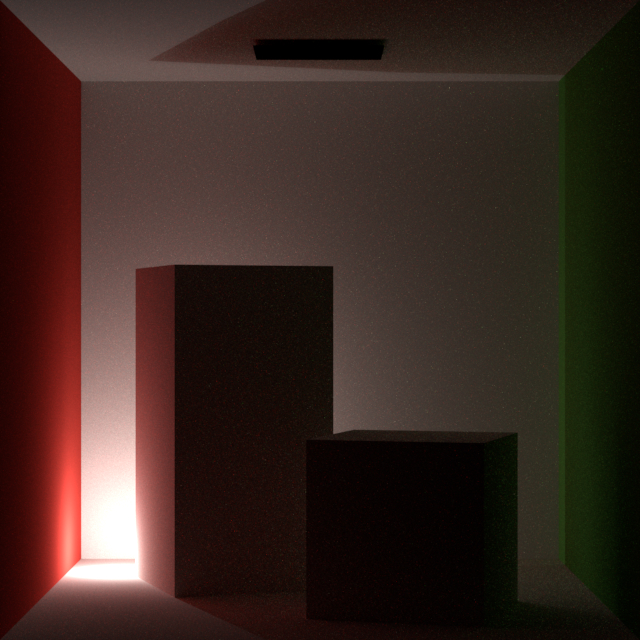
\includegraphics[width=\textwidth]{images/02-linear_lt_light02.jpg}
        \caption*{\(a = 0.0\), \(b = 1.0\)}
        %\label{}
    \end{subfigure}
    \hfill
    \begin{subfigure}[b]{0.24\textwidth}
        \centering
        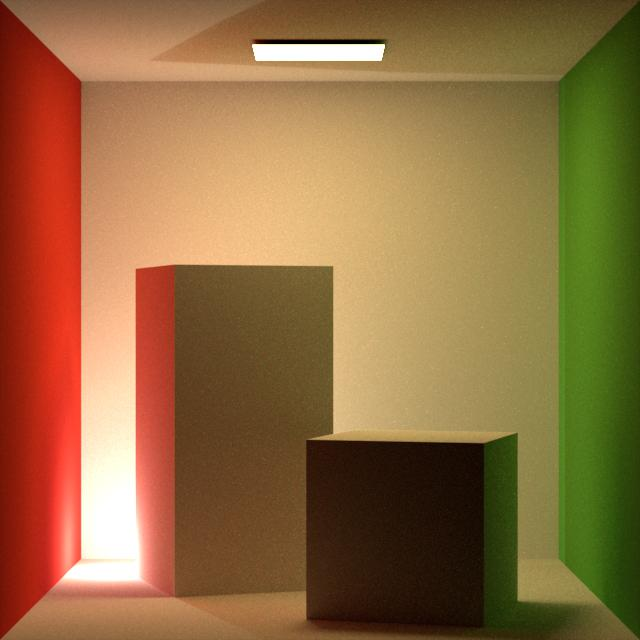
\includegraphics[width=\textwidth]{images/02-linear_lt_comb.jpg}
        \caption*{\(a = 1.0\), \(b = 1.0\)}
        %\label{}
    \end{subfigure}
    \hfill
    \begin{subfigure}[b]{0.24\textwidth}
        \centering
        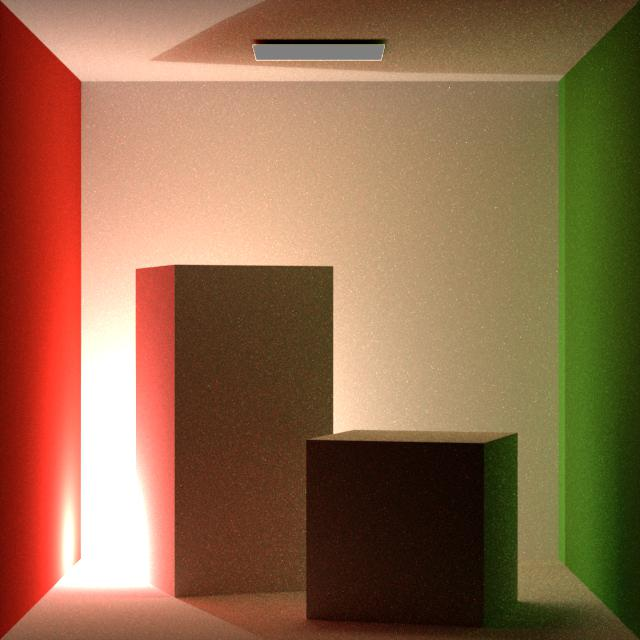
\includegraphics[width=\textwidth]{images/02-linear_lt_comb2.jpg}
        \caption*{\(a = 0.5\), \(b = 2.0\)}
        %\label{}
    \end{subfigure}
    \caption{Demonstration of the linearity of light transport. The scene displayed here has two light sources: on the ceiling and in the back corner. This means that its light transport can be captured using two basis images \(x_1\) and \(x_2\). Each of the above images was then created using a linear combination of the basis images: \(a \cdot x_1 + b \cdot x_2\)}
    \label{fig:background_linear_lt}
\end{figure}

As a consequence, radiance incoming onto a given camera sensor can be determined by the \textit{light transport (LT) matrix} \(A\):

\begin{equation}
    \label{eq:lt_matrix}
    A = \begin{bmatrix}
        c_{11} & c_{21} & c_{31} & \dots & c_{m1} \\
        c_{12} & c_{22} & c_{32} & \dots & c_{m2} \\
        c_{13} & c_{23} & c_{33} & \dots & c_{m3} \\
        \vdots & \vdots & \vdots & \ddots & \vdots \\
        c_{1n} & c_{2n} & c_{3n} & \dots & c_{mn}
    \end{bmatrix}
\end{equation}

where \(m\) is the number of light sources in a scene, \(n\) is the number of pixels in the camera sensor and \(c_{ij}\) is the value of the \(j\)-th pixel of an image that was rendered with only the \(i\)-th light source turned on. By taking a linear combination of the columns of the matrix it is then possible to obtain an image rendered by the corresponding combination of light sources.

In projection mapping, this matrix is usually extremely large because \(n\) corresponds to camera resolution and \(m\) corresponds to projector resolution. Also, in colorful images, each \(c_{ij}\) is a 3-dimensional vector. The two main challenges are therefore

\begin{itemize}
    \item Capturing the matrix
    \item Obtaining its inverse
\end{itemize}

In practice, it is impossible to capture the matrix by projecting a canonical basis because this would mean projecting with only a single pixel turned on and the signal-noise ratio of camera sensors is too high to capture such faint light. While it would be possible to project a different basis that is detectable by a camera, such a process would still be very time consuming. Methods for light transport capture usually rely on the fact that the LT matrix is often very sparse. In fact, the less inter-reflection there is in a scene, the sparser the matrix is. One example of a method that reconstructs the matrix using a limited number of samples is \citet{Peers2009}. Using that method it is possible to capture a matrix with \(m = 128^2\) using 991 measurements.

Inverting the matrix (or, more precisely, obtaining its pseudo-inverse because it is not generally square) is also practically impossible due to the size of the matrix. The solution is again to use the sparsity of the matrix to arrive at an estimate.

For example, \citet{Wetzstein2007} use the inverse light transport approach to implement a projection mapping method which works with arbitrary scenes and also compensates projector defocus which previously mentiones methods ignored. The drawbacks of this method are several hours long matrix acquisition process (during and after which the scene needs to stay static) and also the loss of some global illumination effects caused by estimates of both the LT matrix and its pseudo-inverse. Example results can be seen in fig. \ref{fig:background_wetzstein_result}.

\begin{figure}[ht]
    \centering
    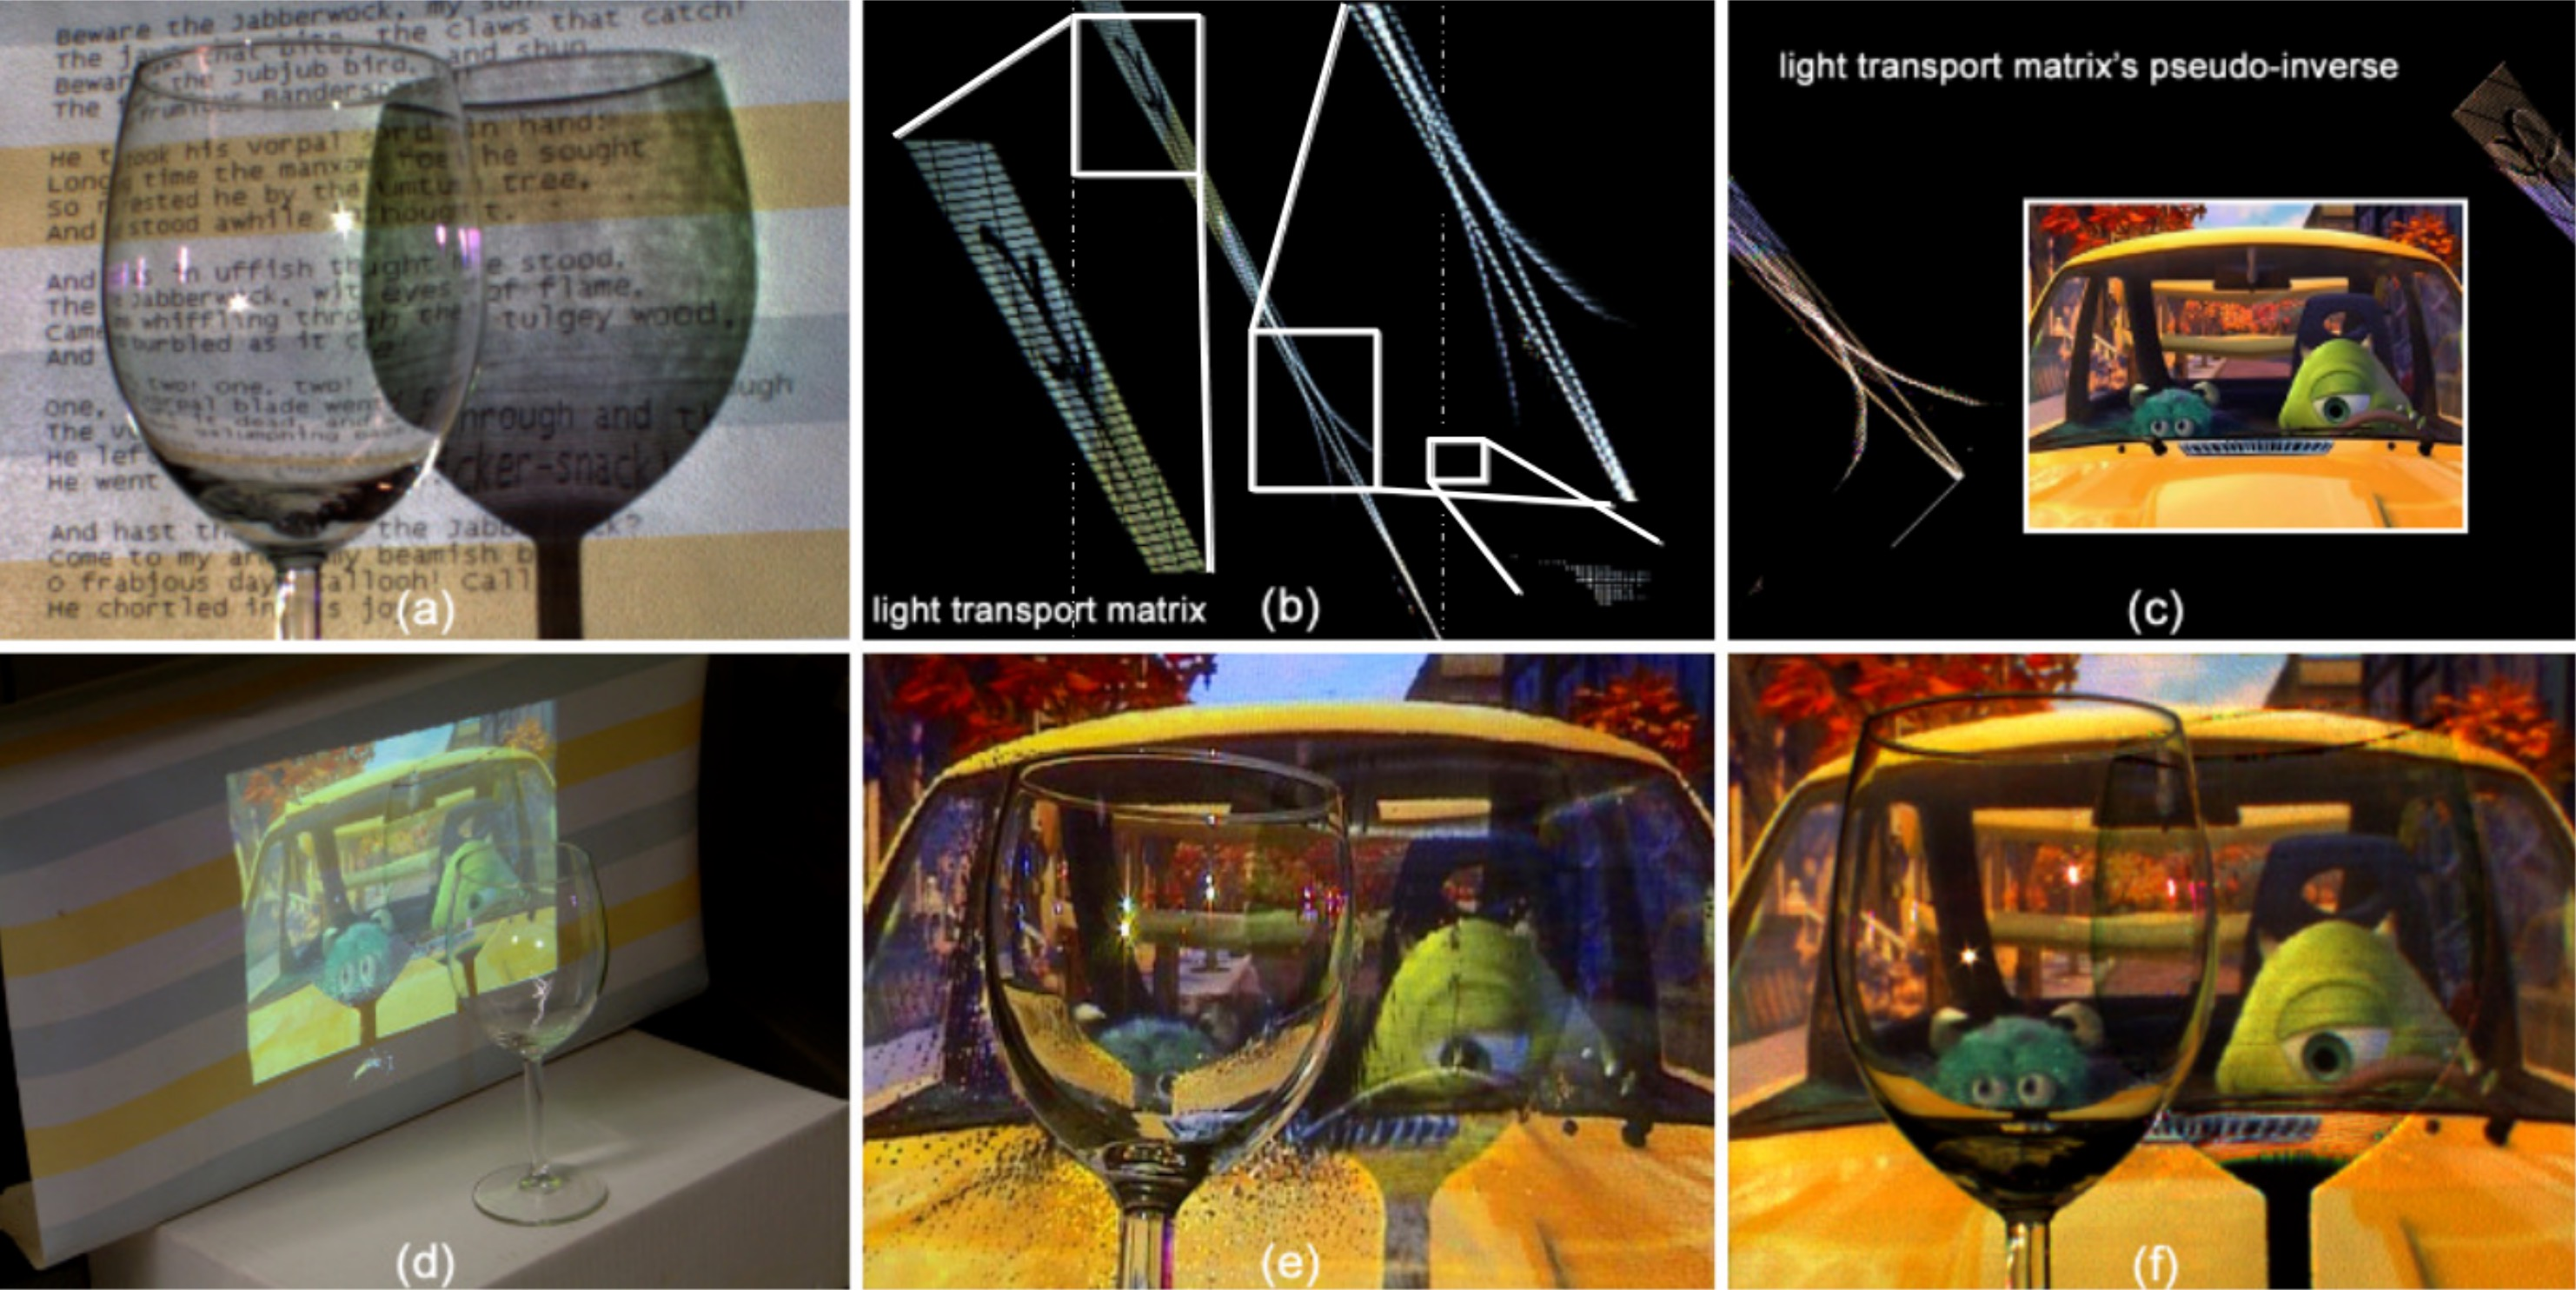
\includegraphics[width=0.8\textwidth]{images/02-wetzstein_result_compressed.jpg}
    \caption{Results of a projection mapping method by \citet{Wetzstein2007}. A wine glass in front of a colored wallpaper (a). The light transport matrix’s (b) pseudo-inverse (c, background) is approximated with a clustering scheme and allows a real-time compensation for displaying interactive content and movies (c) - from an angle (d), compensated with a conventional method (e) and with inverse light transport (f). Source: \citet{Wetzstein2007}}
    \label{fig:background_wetzstein_result}
\end{figure}

This concludes the section on projection mapping which was aiming to explain how to predict what an image will look like when projected onto a scene. We now move on to the second topic that our method builds on. This time we focus on what a texture is and how to generate new realizations of a given texture sample.

\section{Texture Synthesis}
\label{section:background-texture_synthesis}

As mentioned in section \ref{section:intro-key_idea}, the aim of this thesis is to advance the idea of content-based projection mapping of textures. As section \ref{section:background-projection_mapping} suggests, with current projector hardware it is not always possible to match the camera image with the desired appearance pixel by pixel while minimizing clipping errors. Hence in our method we loosen up the definition of image similarity. Textures are a great candidate to start with because two textures can have radically different pixel values in corresponding position but still look the same (see fig. \ref{fig:background_similar_textures} for an example).

\begin{figure}[ht]
    \centering
    \begin{subfigure}[b]{0.48\textwidth}
        \centering
        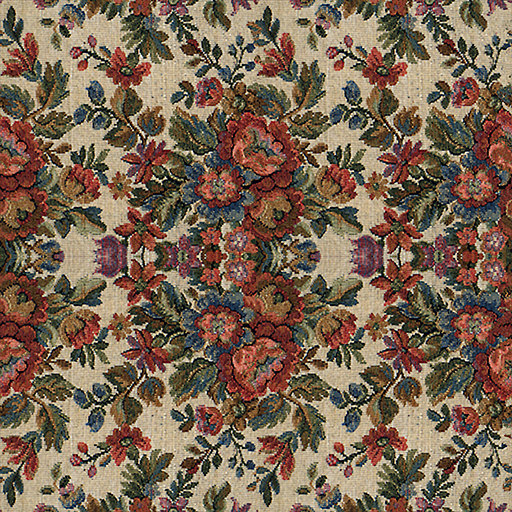
\includegraphics[width=\textwidth]{images/02-flowers1.png}
        \caption*{}
        %\label{}
    \end{subfigure}
    \hfill
    \begin{subfigure}[b]{0.48\textwidth}
        \centering
        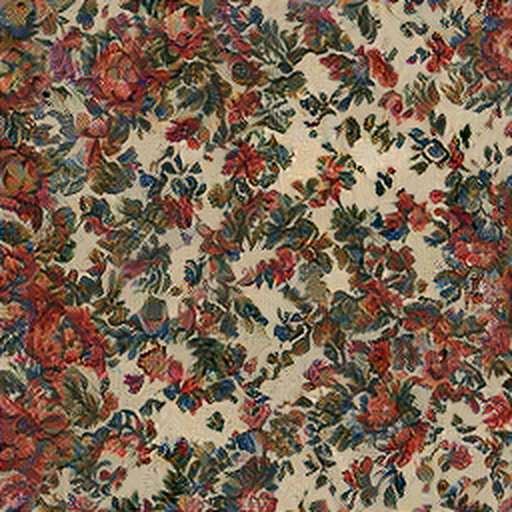
\includegraphics[width=\textwidth]{images/02-flowers2.png}
        \caption*{}
        %\label{}
    \end{subfigure}
    \caption{An example of two realizations of the same texture. The image on the right was created by a texture synthesis method of \citet{Gatys2015}. Texture source: \citet{Pixar128}, modified}
    \label{fig:background_similar_textures}
\end{figure}

But what exactly is a texture and what kind of image modifications can be done while preserving it? In this section, we provide an overview of texture synthesis research which is the second building block that our method relies on.

\subsection{Textures}
\label{section:background-texture_synthesis-textures}

Figures \ref{fig:intro_pixels_vs_stats} and \ref{fig:background_similar_textures} show examples of textures. Unfortunately, according to \citet{Raad2018} there is no universally accepted mathematical definition of what constitues a texture. Researchers who have attempted to characterize textures have usually defined them in terms of human vision. For example, \citet{Julesz1962}, one of the most prominent researchers in this field, has defined textures as classes of images that cannot be discriminated in preattantive (i.e. effortless or instantaneous) vision and then attempted to characterize them mathematically.

How should then one go about doing texture synthesis (i.e. generating new examples of a given texture class) when there is no formal definition of what a texture is? Existing methods can be divided into two categories based on how they approach this problem:

\begin{enumerate}
    \item Find a new candidate for texture definition which forms a texture model and then generate images according to that model. This category is also called \textit{parametric texture synthesis} or \textit{statistics-based texture synthesis} (because the models are usually statistical)
    \item Work without a model and instead define a procedure that turns a given texture example into a new one. This category is also called \textit{non-parametric texture synthesis} or \textit{patch-based texture synthesis} (because the procedure usually generates the texture image patch by patch)
\end{enumerate}

In the following sections we explain the theoretical background of both approaches to texture synthesis and describe the most important methods in each category. Specifically, we focus on strengths and weaknesses of each method and on how suitable it is for our purpose of projection mapping of textures as outlined in section \ref{section:intro-key_idea}. For a more in-depth review of the state of the art in texture synthesis, see \citet{Raad2018}.

\subsection{Patch-Based Texture Synthesis}
\label{section:background-texture_synthesis-patch_based}

We begin with patch-based texture synthesis because it is conceptually simpler and achieves very good results for particular kinds of textures. The basic idea was introduced by \citet{Efros1999} and was inspired by \citet{Shannon1948} and his use of a Markov chain to generate English text. Here is an example of Shannon's method (taken from \citet{Raad2018}):

\begin{itemize}
    \item in no ist lat whey cratict froure birs grocid pondenome of demonstures of the reptagin is regoactiona of cre
\end{itemize}

Analogously to two different texture realizations, this sentence is not English, but looks like it. It is generated letter by letter by sampling from a probability distribution of an English text sample conditioned on the previous \(n = 3\) letters.

In their texture synthesis method, \citet{Efros1999} generate an image pixel by pixel based on a probability distribution of the given texture sample. We will desribe how exactly this method works on an improved version of it, called \textit{image quilting}, which was introduced by \citet{Efros2001}.

\subsubsection{Image Quilting}
\label{section:background-texture_synthesis-patch_based-quilting}

\begin{figure}[ht]
    \centering
    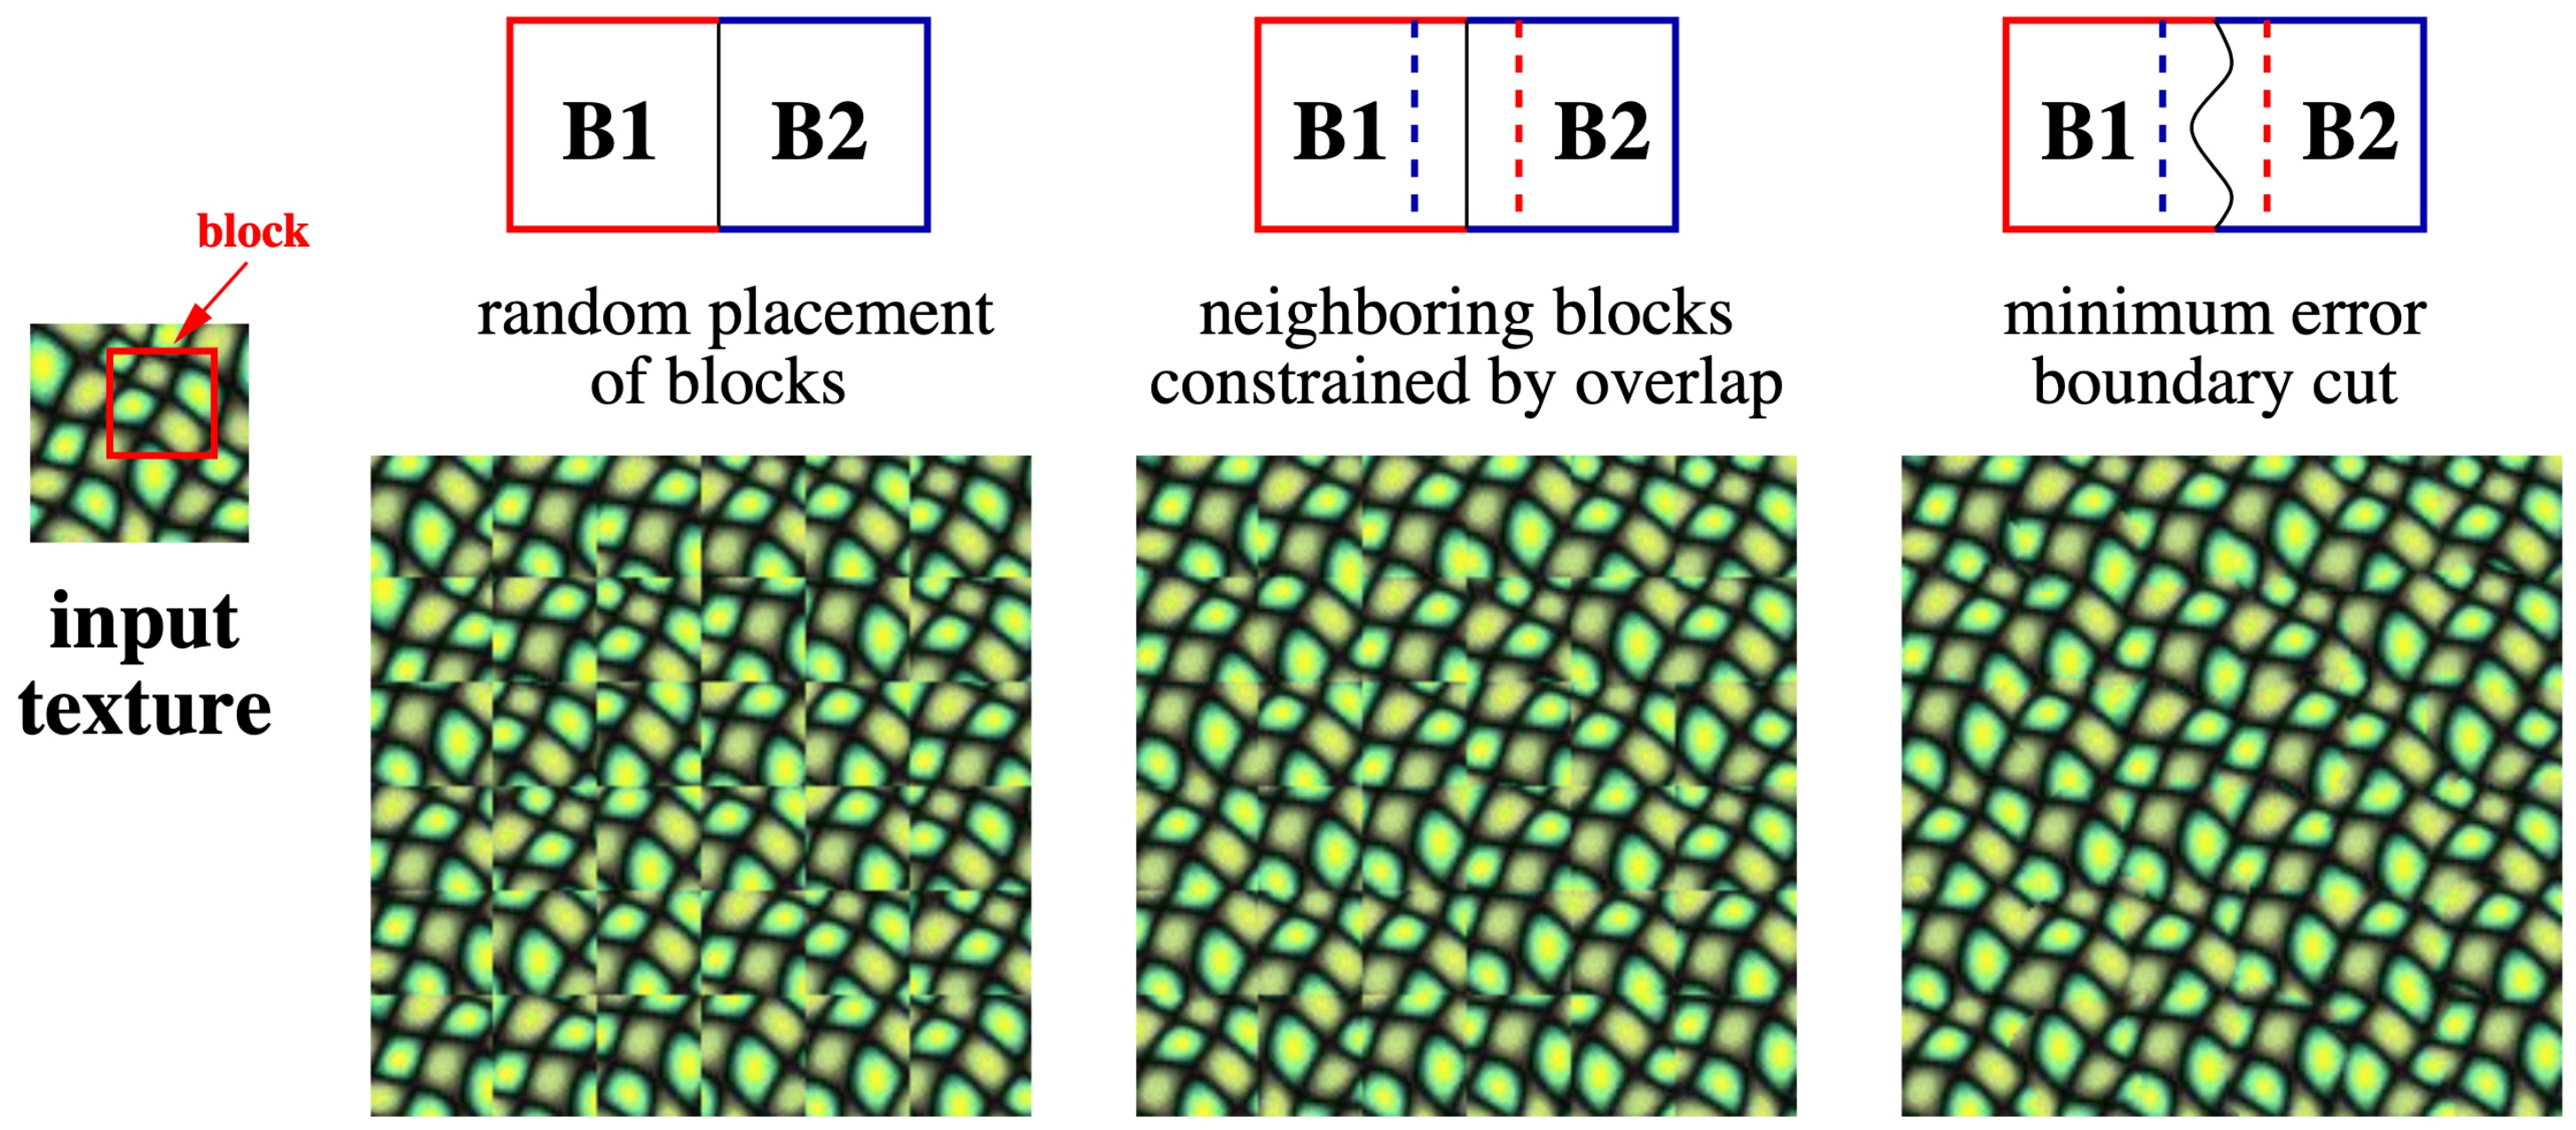
\includegraphics[width=\textwidth]{images/02-quilting_method_compressed.jpg}
    \caption{Illustration of image quilting. The leftmost image was generated by choosing block \(B_i\) at random. The middle image was generated by choosing a block with low pixel-wise error in an overlap with the previous block. The rightmost image was generated by choosing blocks as in the middle, only the new block is pasted along a minimum error path instead of a straight line.  Source: \citet{Efros2001}}
    \label{fig:background_quilting_method}
\end{figure}

Image quilting starts by splitting the input texture image into overlapping square blocks \(B_i\) of size \(k\) (a user-controlled parameter). Then it builds a new texture block by block in raster scan order (from the top left corner to the bottom right corner, row by row). A new block \(B^{\prime}\) is chosen at random from all \(B_i\) such that the pixel-wise error in overlapping areas (they use 1/6 of block area along the edge) with the block above \(B^{\prime}\) and to the left of \(B^{\prime}\) in below a certain threshold in the output image. Since many blocks usually satisfy this overlap constraint, one is picked at random. If \(B^{\prime}\) was pasted into the output image directly, the result would look blocky. Therefore \(B^{\prime}\) is pasted into the output image along a minimum error path inside the overlapping areas. This ensures that seams between block will be as subtle as possible. See fig. \ref{fig:background_quilting_method} for an illustration of the method.

\subsubsection{Pros and Cons}
\label{section:background-texture_synthesis-patch_based-pros_and_cons}

This method can achieve stunning visual results when the input texture is uniformly lit and contains large features, like pebbles or coffee beans. It is especially powerful when used on textures with regular structure, like a brick wall. See fig. \ref{fig:background_quilting_pros_cons} for an example.

However, it struggles with textures that have non-uniform illumination and that contain very small features, like sand or concrete. Failure cases usually manifest themselves by large areas that are directly copied from the input (so-called \textit{verbatim copying}) or areas that contain the same patch copied over and over (so-called \textit{garbage growing}). See fig. \ref{fig:background_quilting_pros_cons} for an example.

\begin{figure}[ht]
    \centering
    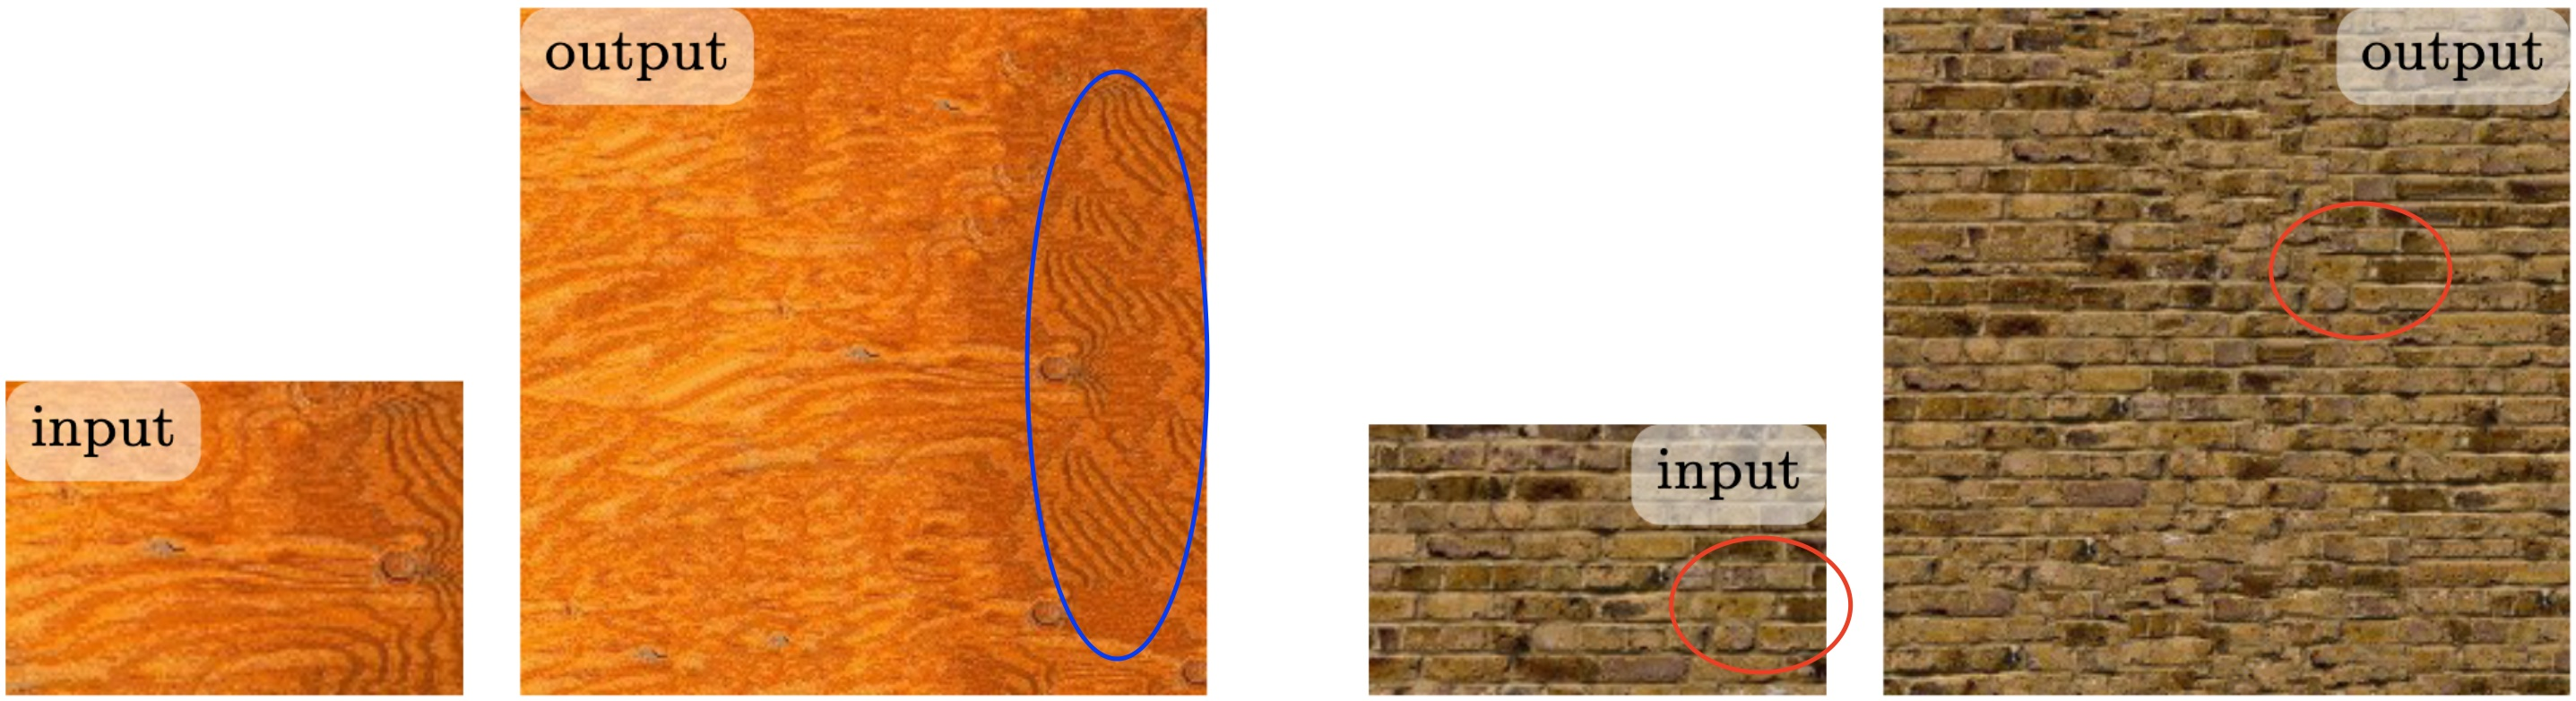
\includegraphics[width=\textwidth]{images/02-quilting_pros_cons_compressed.jpg}
    \caption{Examples of image quilting. On the left is a failure with the garbage growing effect highlighted in blue. On the right is a success. However, some verbatim copies (highlighted in red) are clearly visible in the rightmost image. Source: \citet{Raad2018}, highlighting own}
    \label{fig:background_quilting_pros_cons}
\end{figure}

Another drawback of this method is that its parameters need to be manually tuned based on the feature sizes and other properties of the input texture. There is also no underlying texture model that this method would work with which means that reasoning about it is somewhat less robust and limited to measuring heuristics such as the amount of verbatim copies and garbage in the output.

\subsubsection{Potential Usage in Projection Mapping}
\label{section:background-texture_synthesis-patch_based-projection_mapping}

Image quilting is surprisingly flexible to adapt for other uses than texture synthesis. The authors themselves showcase the possibility of using the method for style transfer. This is a problem that considers two input images and produces a third one which has the content of one image and style of the other. This can be achieved by adding a new term to the overlap error. In the case of style transfer, it takes the form of the difference in pixel intensities of the candidate patch and a corresponding patch of the target image. See fig. \ref{fig:background_quilting_transfer} for an example.

\begin{figure}[ht]
    \centering
    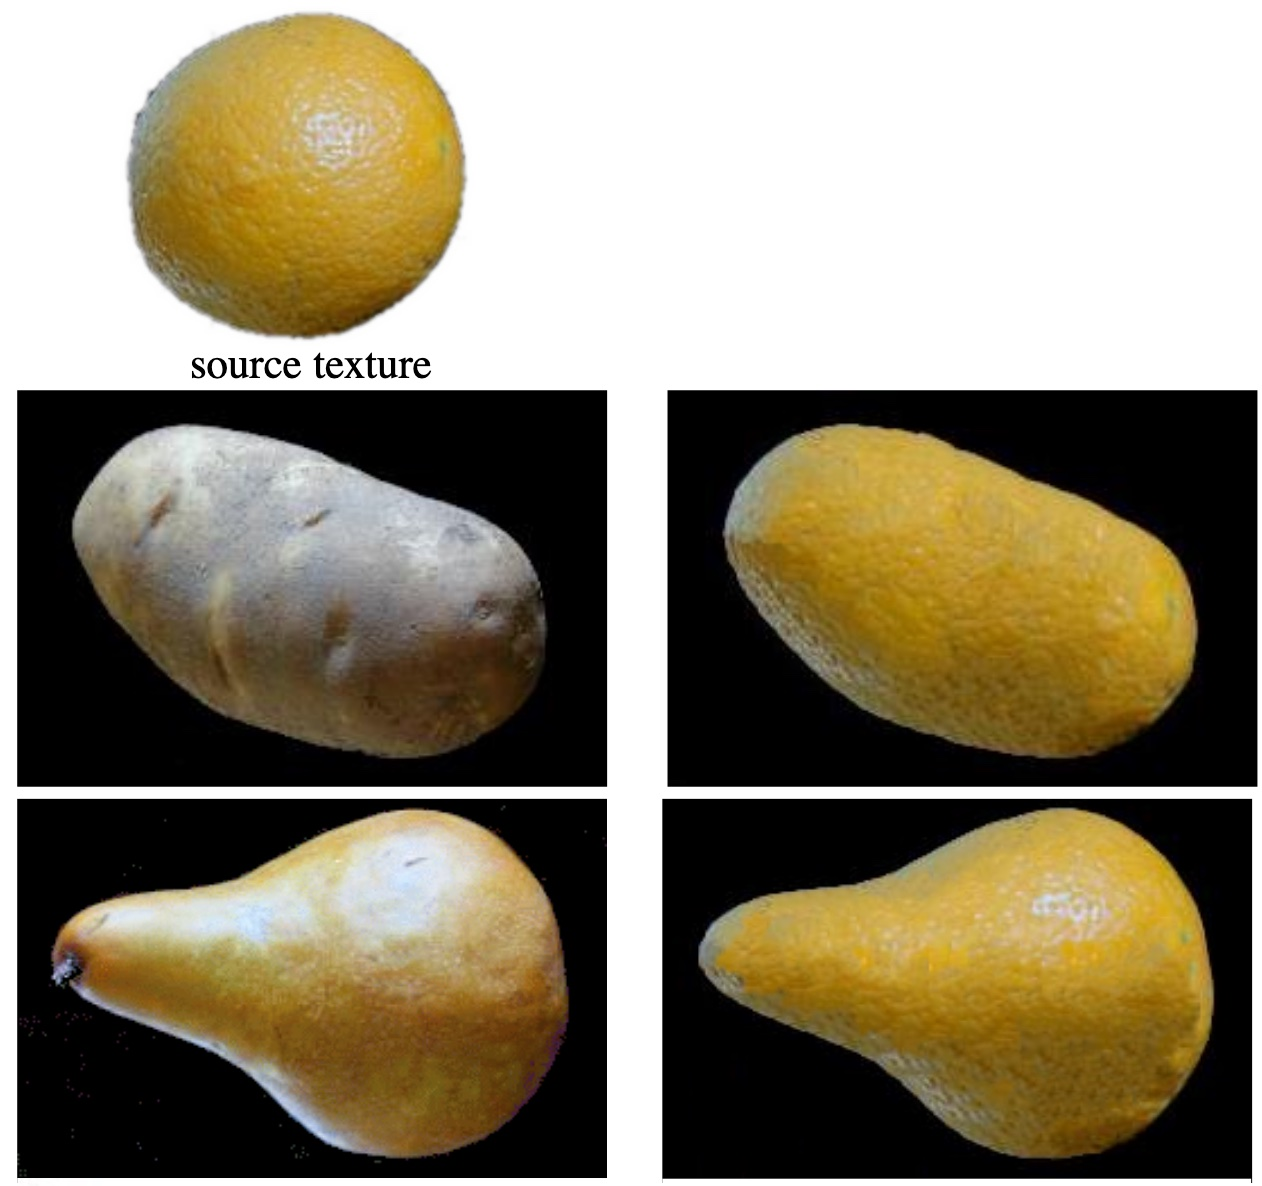
\includegraphics[width=0.6\textwidth]{images/02-quilting_transfer_compressed.jpg}
    \caption{Example of style transfer using image quilting. The output (right) is generated just like during texture synthesis except for two changes: 1) the output image size is chosen to be that of the target image (left) and 2) an extra term is added to the overlap error. This term represents the difference between the pixel intensities of the candidate patch and a corresponding patch of the target image. Source: \citet{Efros2001}}
    \label{fig:background_quilting_transfer}
\end{figure}

One could imagine using this method for projection mapping by modifying the overlap error term. Roughly speaking, the additional error term could be proportional to how difficult it would be to radiometrically compensate the candidate patch. More specifically, the candiate patch would first be radiometrically compensated and then the error would be set to the inverse distance of the compensation and the limit of the projector gamut. This could be built on top of methods such as \citet{Grundhofer2015} that assume 1:1 correspondence between projector image and camera image.

\subsection{Statistics-Based Texture Synthesis}
\label{section:background-texture_synthesis-statistics_based}

\begin{figure}[ht]
    \centering
    \begin{subfigure}[b]{0.3\textwidth}
        \centering
        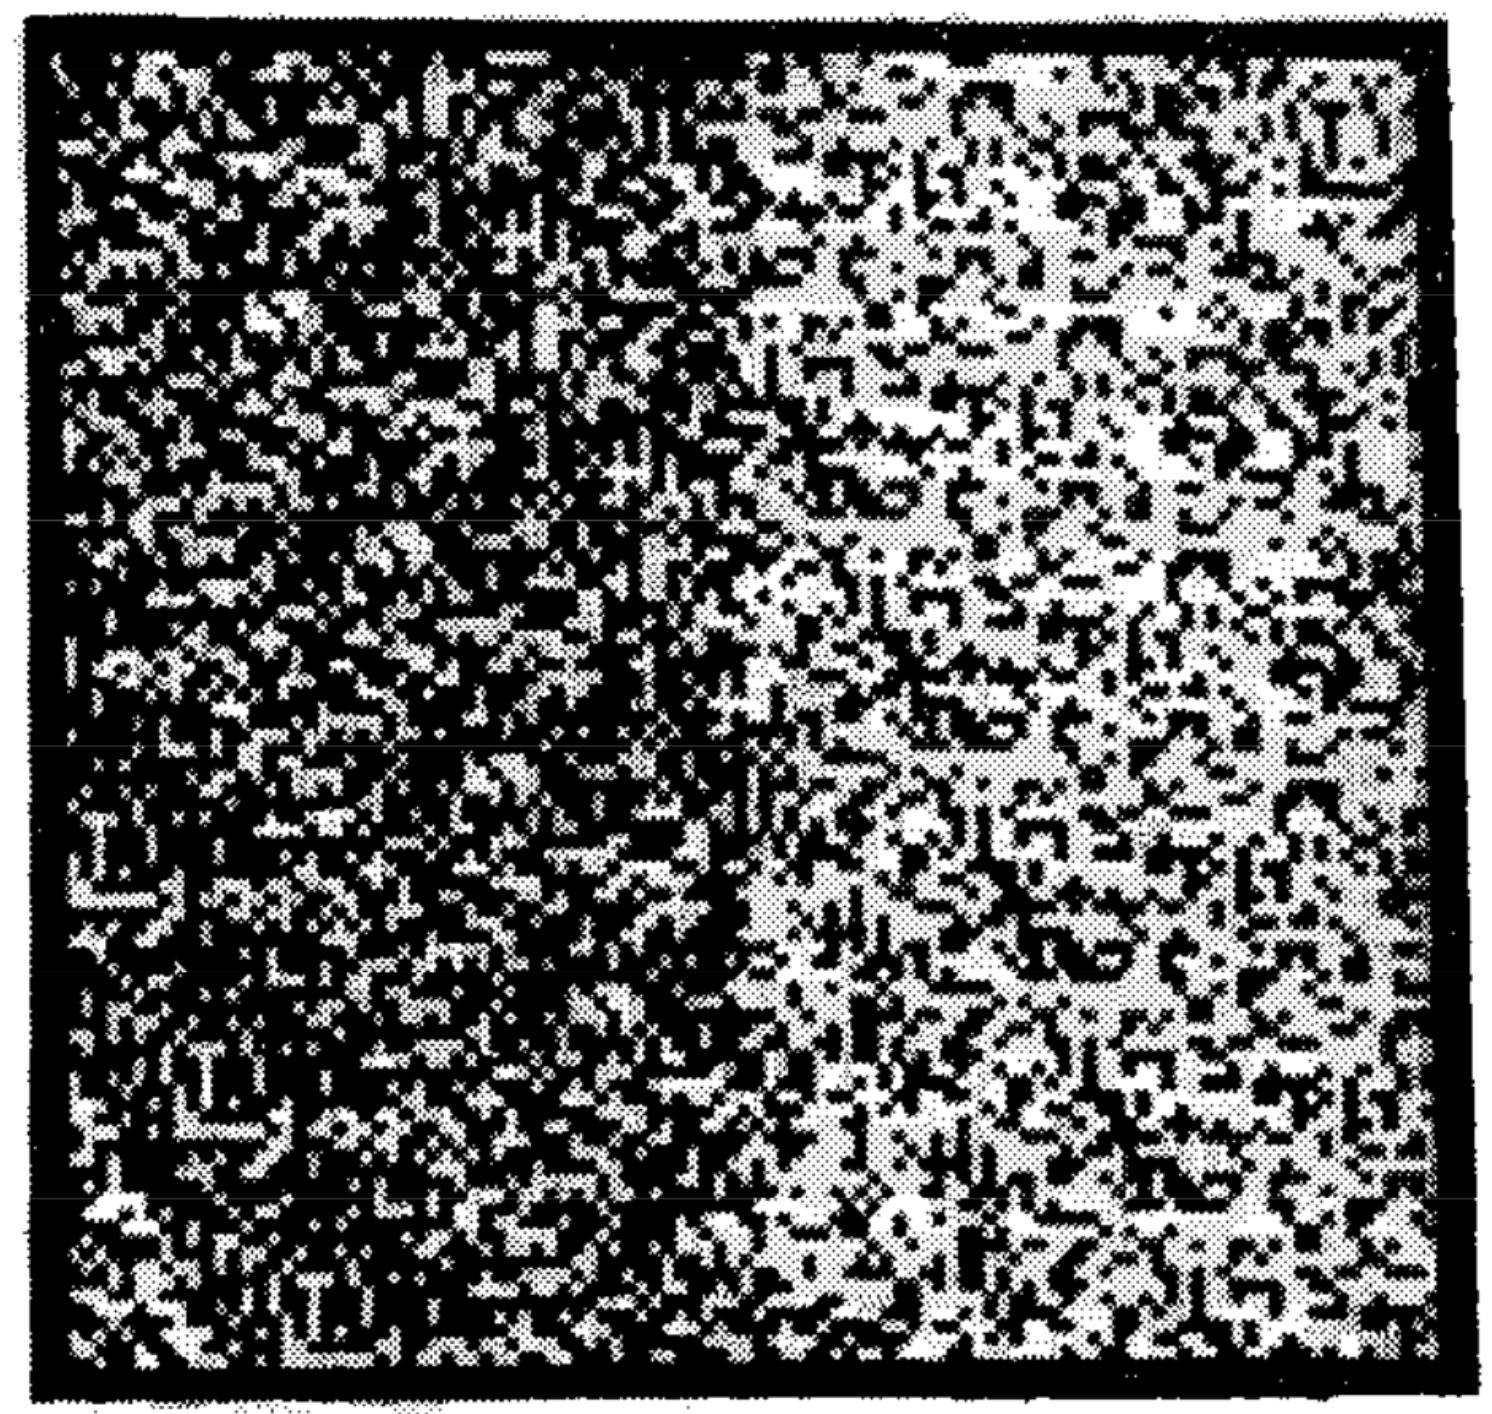
\includegraphics[width=\textwidth]{images/02-julesz-1st_order_compressed.jpg}
        \caption{}
        %\label{}
    \end{subfigure}
    \hfill
    \begin{subfigure}[b]{0.29\textwidth}
        \centering
        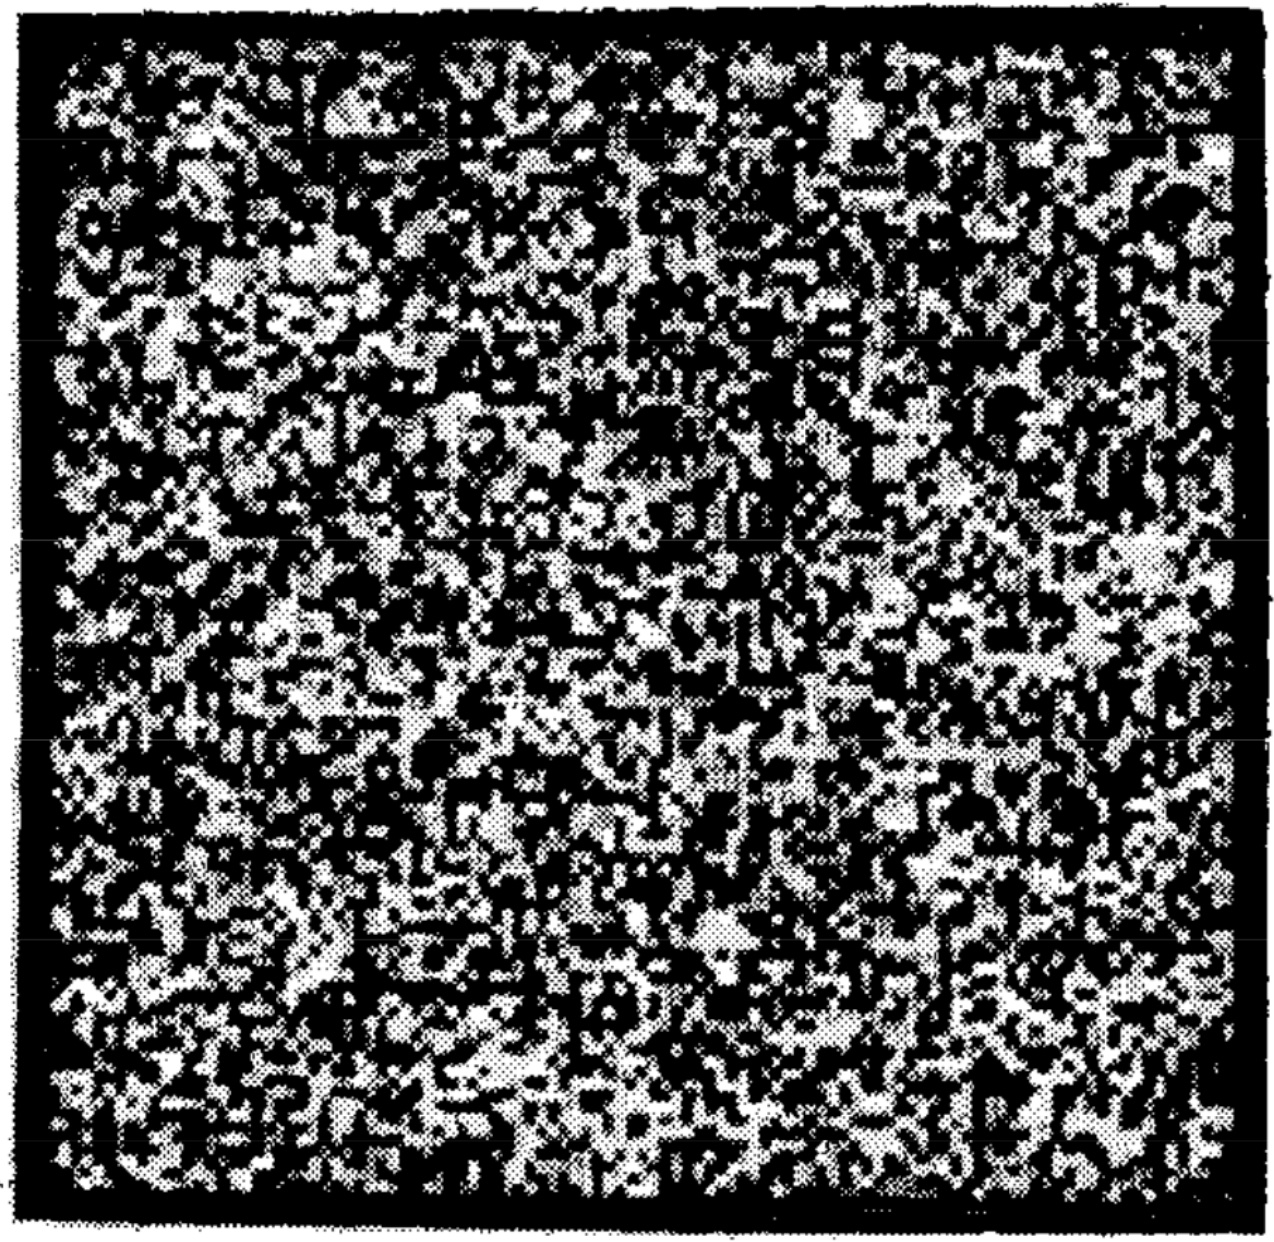
\includegraphics[width=\textwidth]{images/02-julesz-2nd_order_compressed.jpg}
        \caption{}
        %\label{}
    \end{subfigure}
    \hfill
    \begin{subfigure}[b]{0.39\textwidth}
        \centering
        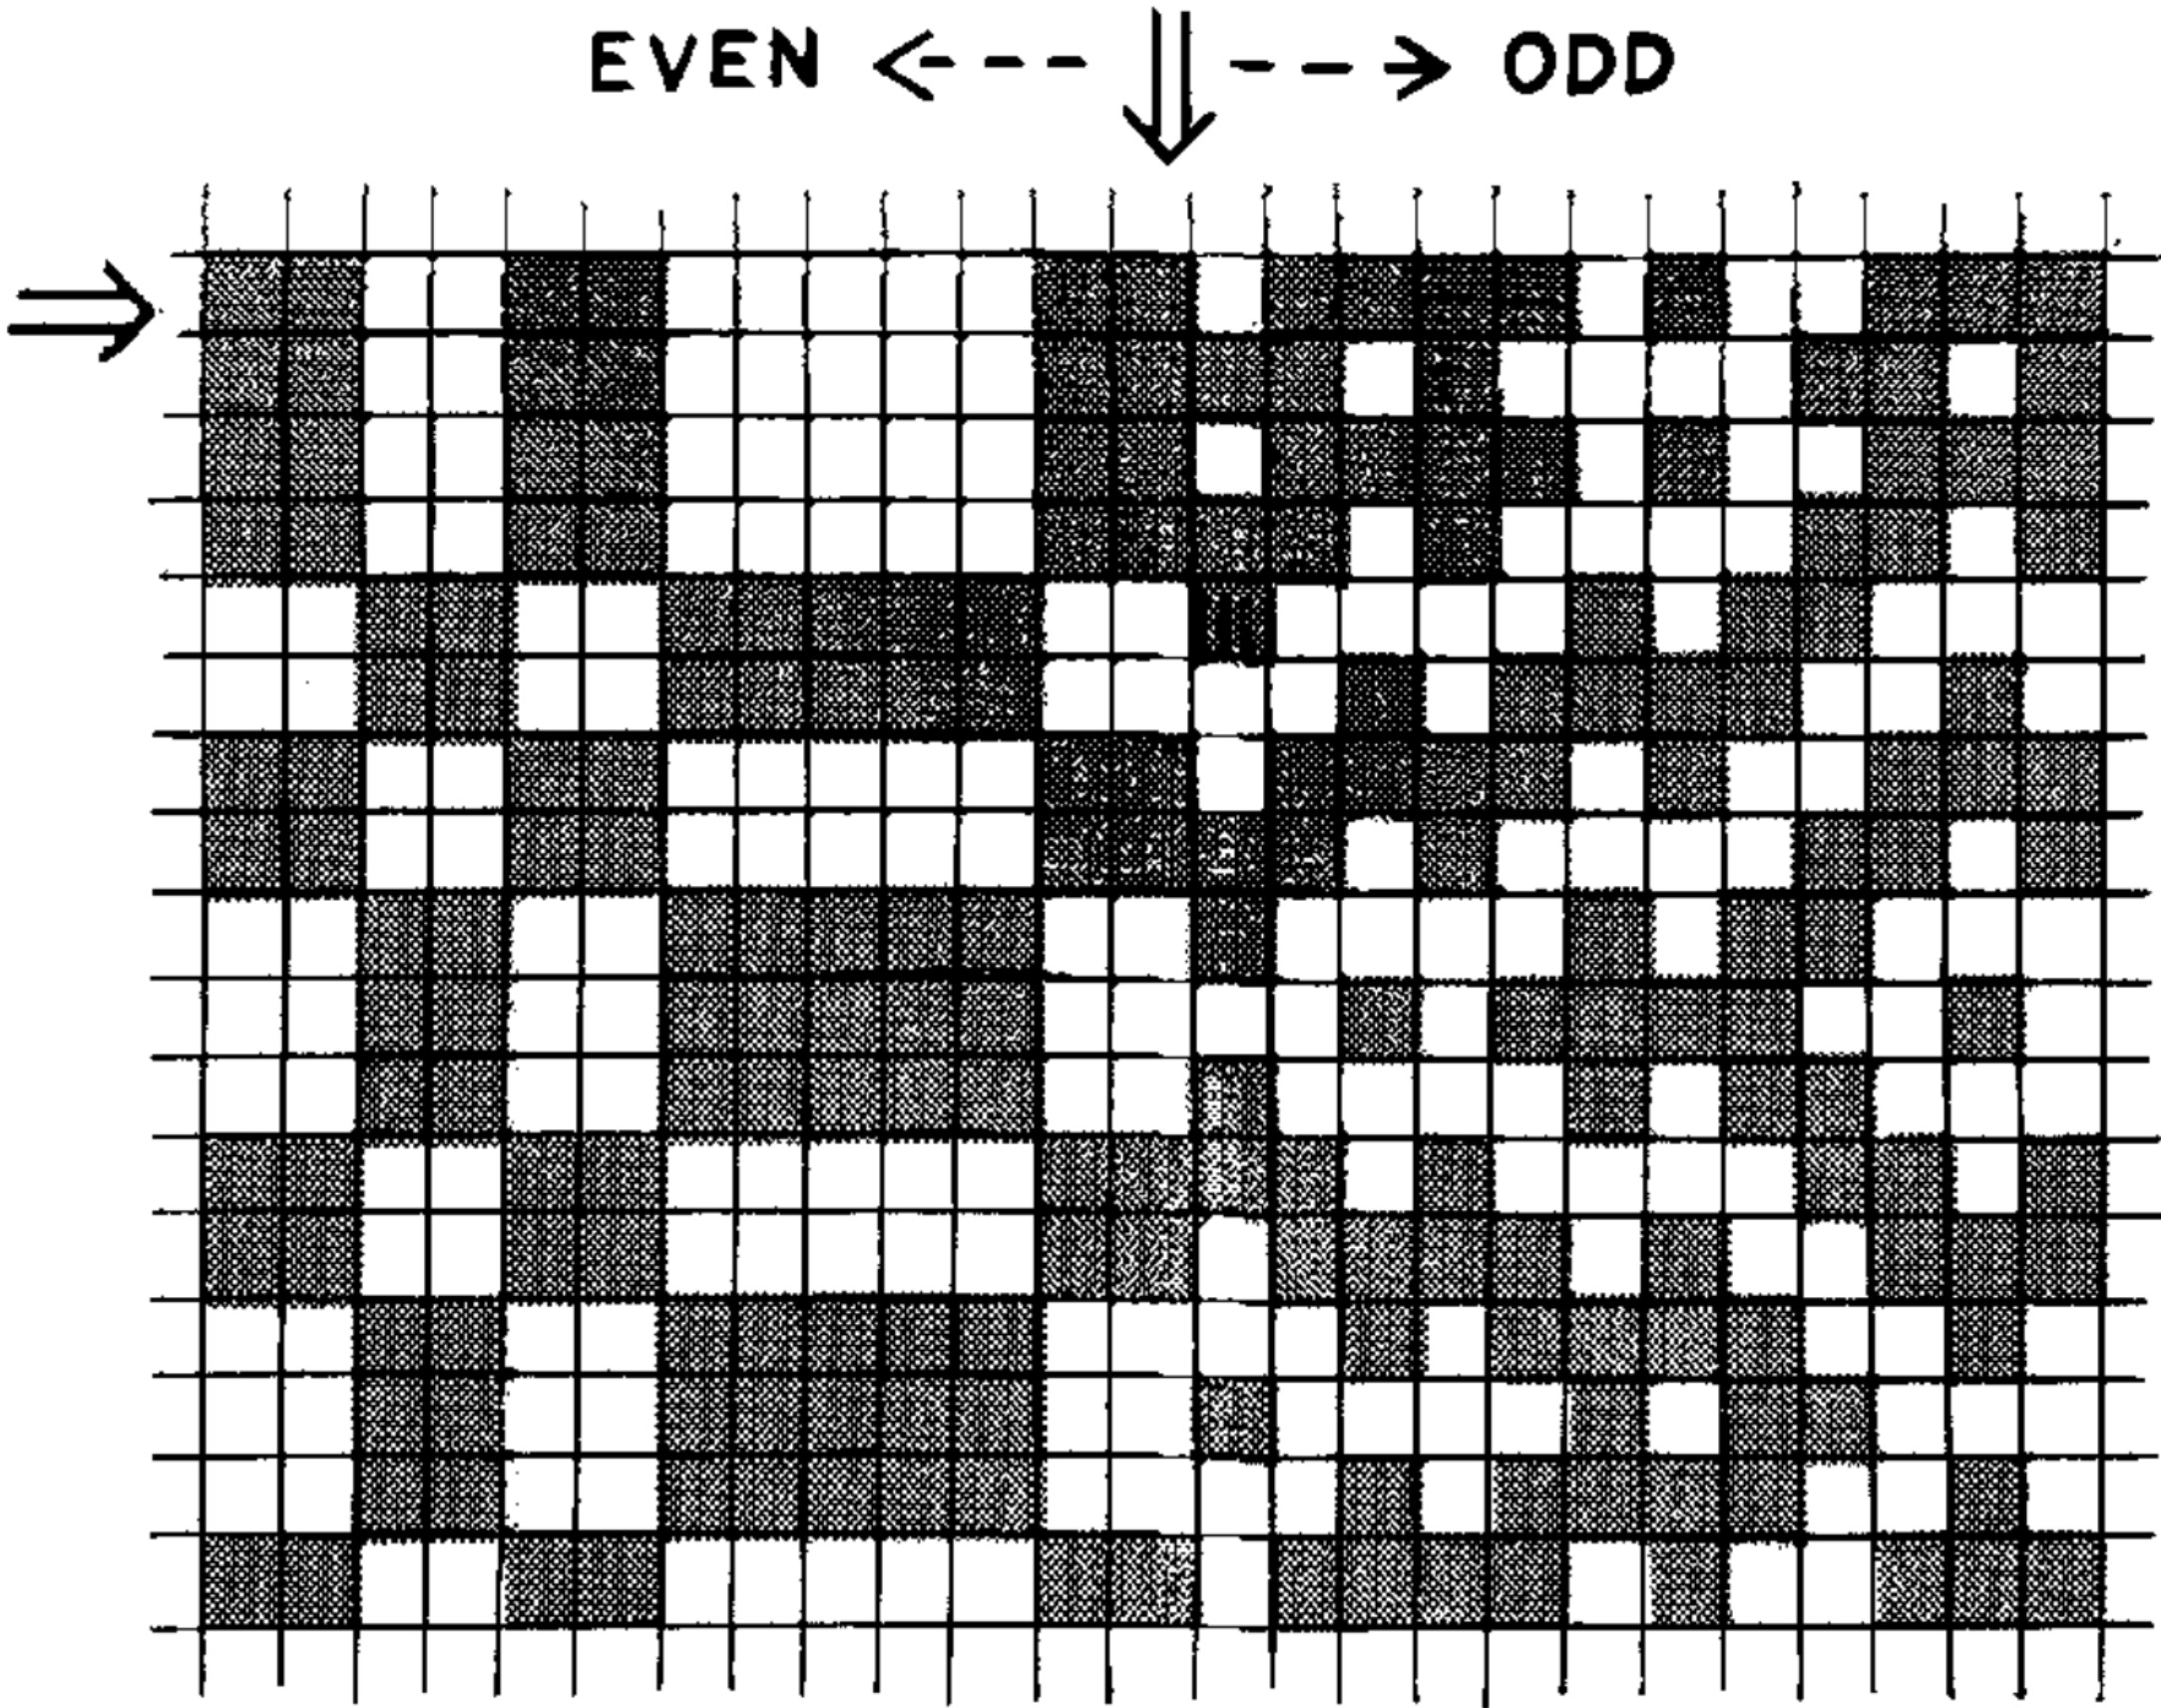
\includegraphics[width=\textwidth]{images/02-julesz-3rd_order_compressed.jpg}
        \caption{}
        %\label{}
    \end{subfigure}
    \caption{Image a) shows two textures with different first-order statistics. The left half contains black pixels with probabilty \(5/8\) and white pixels with probability \(3/8\) while the right half has the inverse distribution. Image b) shows two textures with identical second-order statistics. Specifically, there are four brightness levels in the image each with equal probability (first-order). Moreover, any two pixels are chosen independently (second-order). However, the probability \(P(k | i,j)\) of a pixel conditioned on two other pixels differs between the left and right half which makes third-order statistics different. Image c) shows two textures with identical third-order statistics, meaning that any three squares are chosen independently. However, the left half has \(2 \times 2\) patches with even number of black squares while the left half has an odd number of black squares per patch. This makes the textures easily distinguishable. Texture sources: \citet{Julesz1962} (a, b) and \citet{Julesz1973} (c)}
    \label{fig:background_julesz_textures}
\end{figure}

Statistics-based texture synthesis is an older and more established approach to generating new realizations of textures because it combines two goals:

\begin{itemize}
    \item Finding a mathematical characterization of textures
    \item Synthesizing new texture examples based on that characterization
\end{itemize}

As mentioned in section \ref{section:background-texture_synthesis}, a formal texture model should be compatible with the notion that textures are classes of images that are indistinguishable in preattentive vision. A famous attempt at such a model was introduced by \citet{Julesz1962} who formulated a hypothesis that two textures with identical second-order statistics are preattentively indistinguishable from each other (see fig. \ref{fig:background_julesz_textures} for an example). This hypothesis was later disproved in \citet{Julesz1973} by counter-examples of distinguishable textures with identical third-order statistics (also fig. \ref{fig:background_julesz_textures}). However, the distinguishing features in those counter-examples are local. A modified Julesz hypothesis says that "the pre-attentive textural system cannot globally compute third- or higher-order statistics" (\citet{Julesz1981}) and the idea that global statistics characterize textures well is still prevalent today. See fig. \ref{fig:background_statistics_example} for an illustration of how global statistics can be used for texture synthesis.

\begin{figure}[ht]
    \centering
    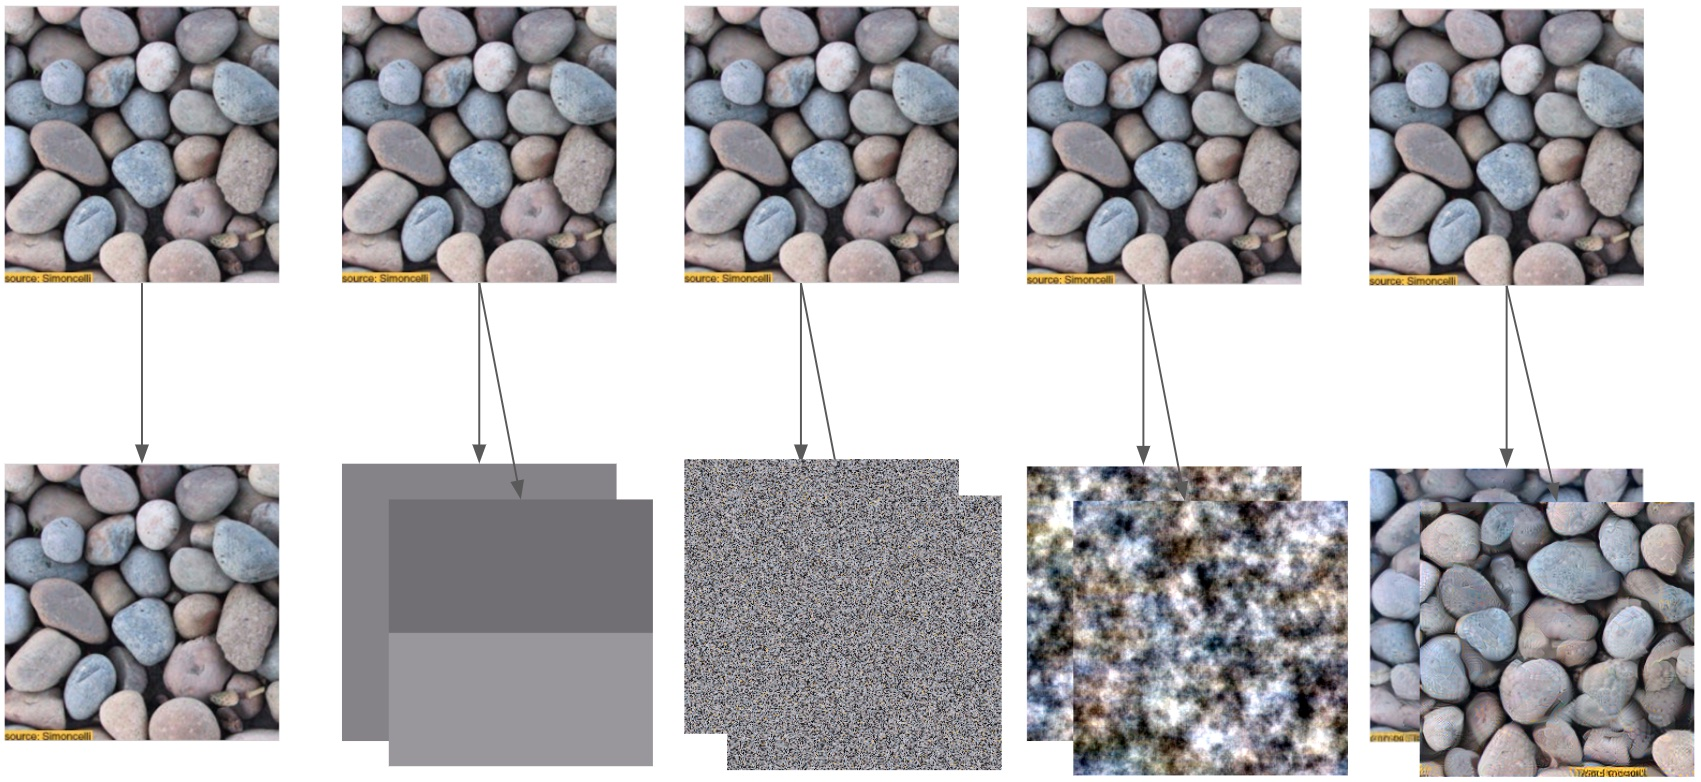
\includegraphics[width=\textwidth]{images/02-statistics_example_compressed.jpg}
    \caption{Illustration of texture synthesis via global image statistics. The leftmost image shows an example generated by keeping every pixel identical. The middle-left image shows an example that uses identical average color as a descriptive statistic. The middle image uses first-ordr statistics by simply shuffling the pixels of the input. The middle-right image uses a method by \citet{Galerne2011} which keeps Fourier modulus identical while randomizing the phase. The rightmost image shows a recent method by \citet{Gatys2015} that uses the Gram matrices of CNN activations as a descriptive statistic. Texture source: \citet{Gatys2015}}
    \label{fig:background_statistics_example}
\end{figure}

In line with the modified Julesz hypothesis, we can see from the examples above that while some synthesis methods are good at creating textures with distinct local features but struggle with more homogeneous texture (e.g. \citet{Efros2001} in fig. \ref{fig:background_quilting_pros_cons}), others are the opposite (e.g. \citet{Galerne2011} and its failure on a macro-texture in fig. \ref{fig:background_statistics_example}). In literature, texture with distinct local features are called \textit{macro-texture} and more homogeneous textures are called \textit{micro-texture}. For a long time there was no method that could reliably generate both types of texture. However, a recent statistics-based method by \citet{Gatys2015} achieves very good results on both micro-textures and macro-textures and we will now provide its overview and explain how it could be used in projection mapping.

\subsubsection{Texture Synthesis Using Convolutional Neural Networks}
\label{section:background-texture_synthesis-statistics_based-synthesis_using_cnns}

\citet{Gatys2015} have introduced a method for texture synthesis that defines a set of statistics that can be computed from an image and then generates new examples of a given texture by imposing those statistics on white noise images. This happens in an optimization loop that minimizes a loss function which represents the difference between the statistics of the generated image and the input texture (see fig. \ref{fig:background_gatys_method} for an illustration).

\begin{figure}[ht]
    \centering
    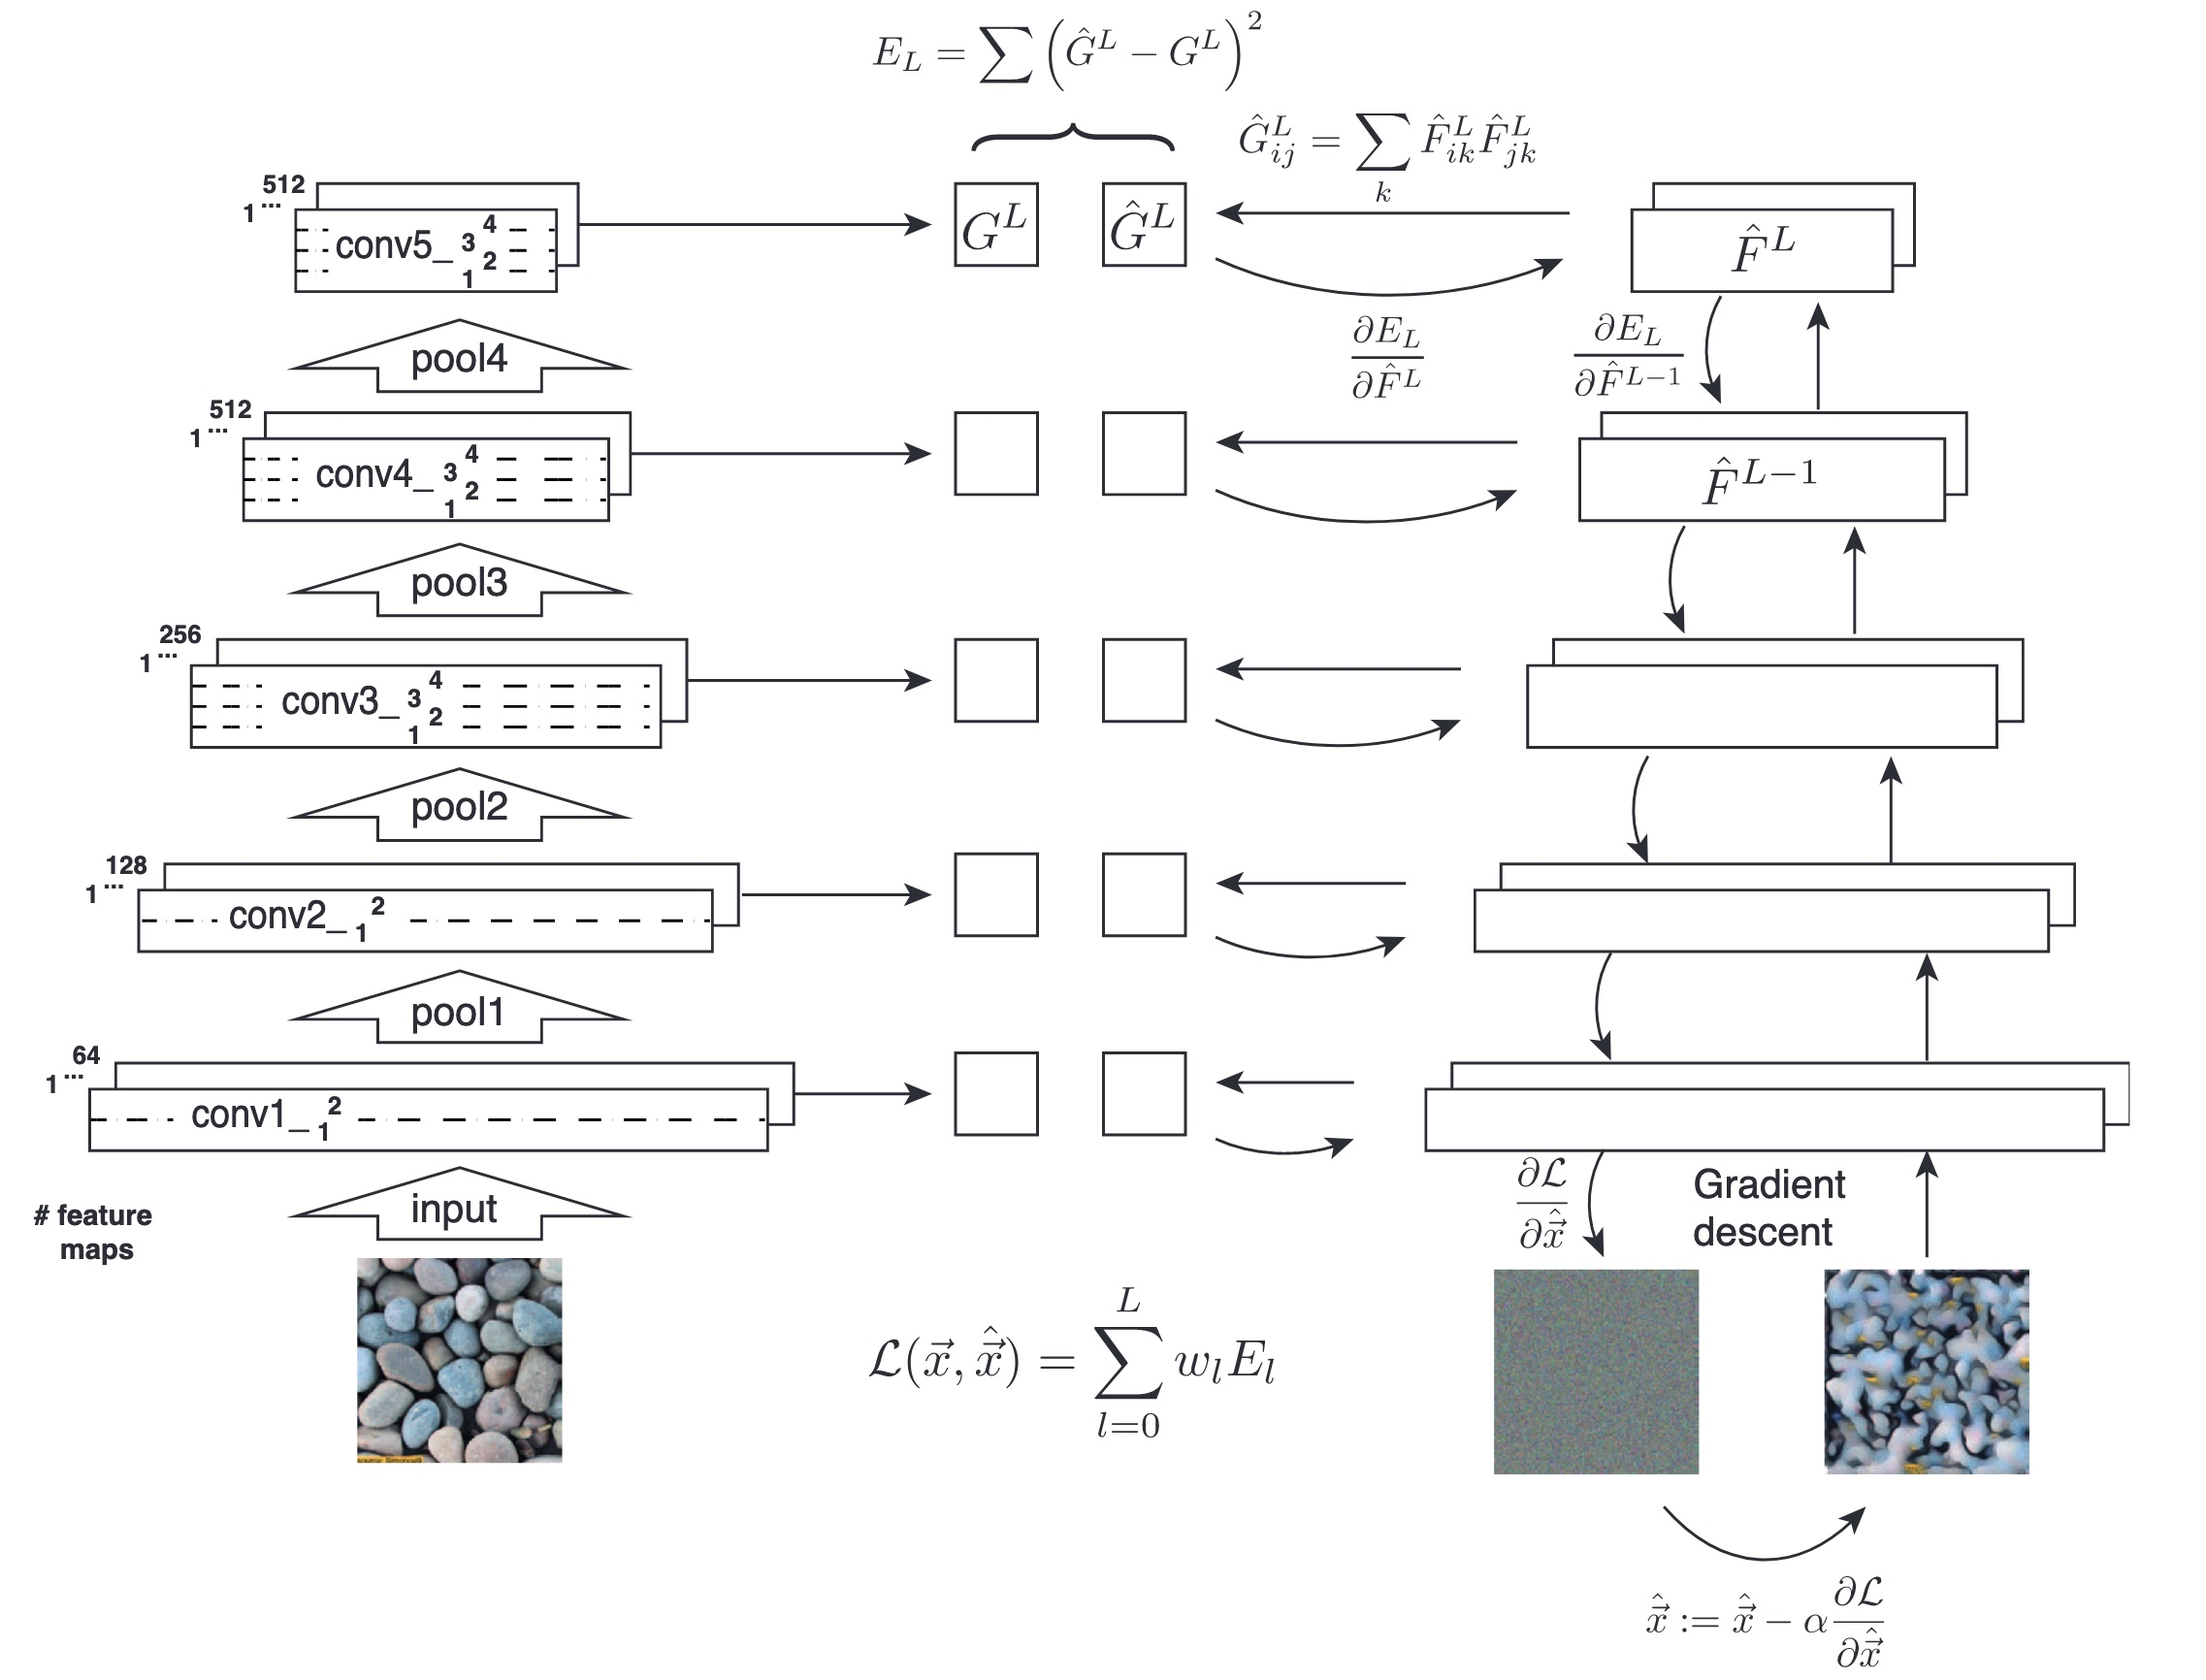
\includegraphics[width=\textwidth]{images/02-gatys_method_compressed.jpg}
    \caption{Illustration of CNN-based texture synthesis by \citet{Gatys2015}. At the bottom we can see the input texture, the initial white noise image and the progressively refined image. The diagram above represents the computation of the CNN activations and their Gram matrices \(G\). The loss \(\mathcal{L}\) that drives the optimization via gradient descent is defined as a weighted sum of the differences between Gram matrices of individual CNN layers. Source \citet{Gatys2015}}
    \label{fig:background_gatys_method}
\end{figure}

The set of statistics is computed using a \textit{convolutional neural network} (abbreviated as CNN and covered in more detail in appendix \ref{chapter:appendix-cnns}) which is trained on an image classification task. It is determined by the activations after each pooling layer of the VGG-19 CNN by \citet{Simonyan2014}. These activations, however, contain spatial information of where each feature is located in the texture. This is not desirable because textures are stationary (i.e. their features can be shuffled around without making them a different texture). In order to remove this spatial information, activations are correlated with each other within each layer, forming a so-called \textit{Gram matrix}. Gram matrices of VGG-19 activations therefore constitute a set of statistics completely describing a texture.

To synthesize a new example of a given texture, gradient-based loss optimization is used. The loss is defined as a weighted mean square error between the statistics the input texture and the image being optimized. The L-BFGS optimizer is used to drive the optimization process. See fig. \ref{fig:background_gatys_method} for an illustration of how this method works.

\subsubsection{Pros and Cons}
\label{section:background-texture_synthesis-statistics_based-pros_and_cons}

\begin{figure}[ht]
    \centering
    \begin{subfigure}[b]{0.8\textwidth}
        \centering
        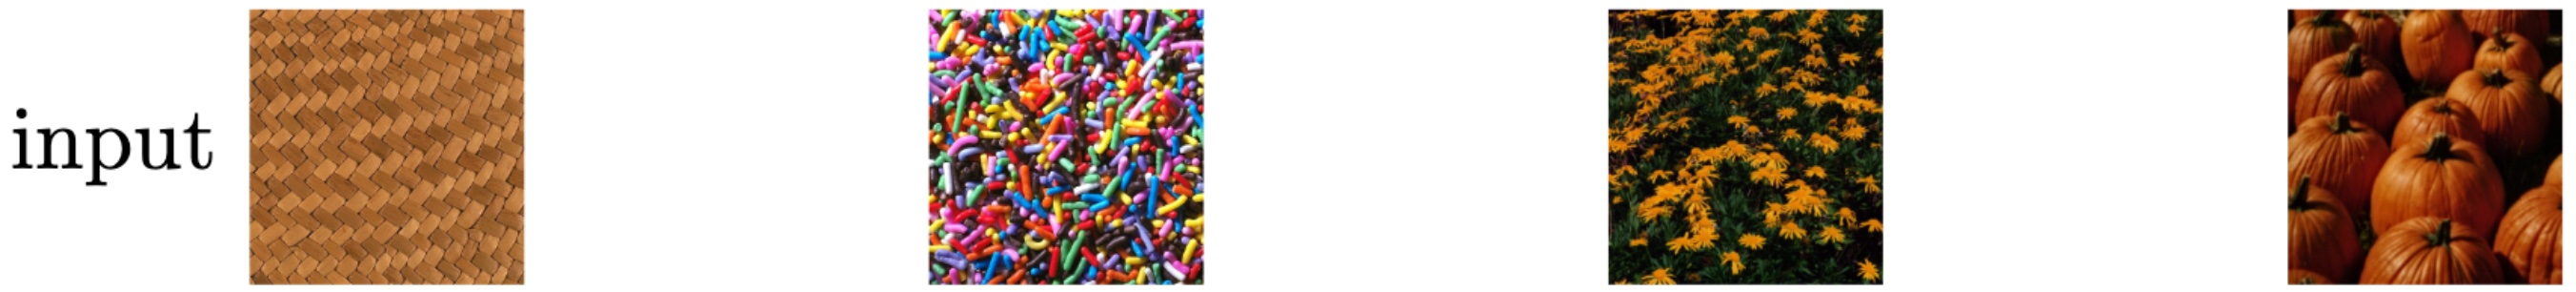
\includegraphics[width=\textwidth]{images/02-big_comparison_input_compressed.jpg}
        \caption*{}
        %\label{}
    \end{subfigure}
    
    \begin{subfigure}[b]{\textwidth}
        \centering
        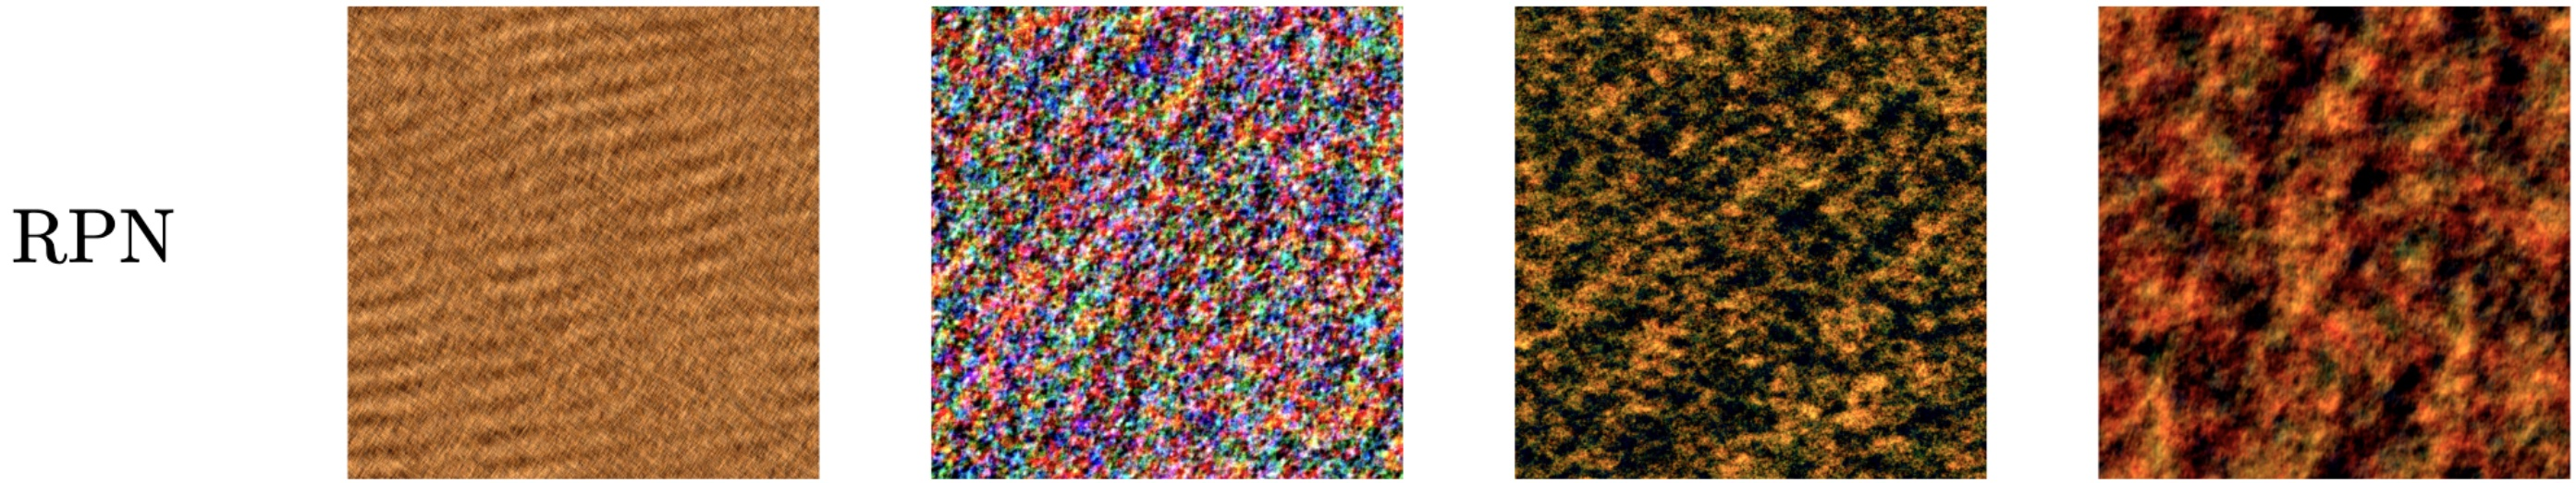
\includegraphics[width=\textwidth]{images/02-big_comparison_rpn_compressed.jpg}
        \caption*{}
        %\label{}
    \end{subfigure}
    
    \begin{subfigure}[b]{\textwidth}
        \centering
        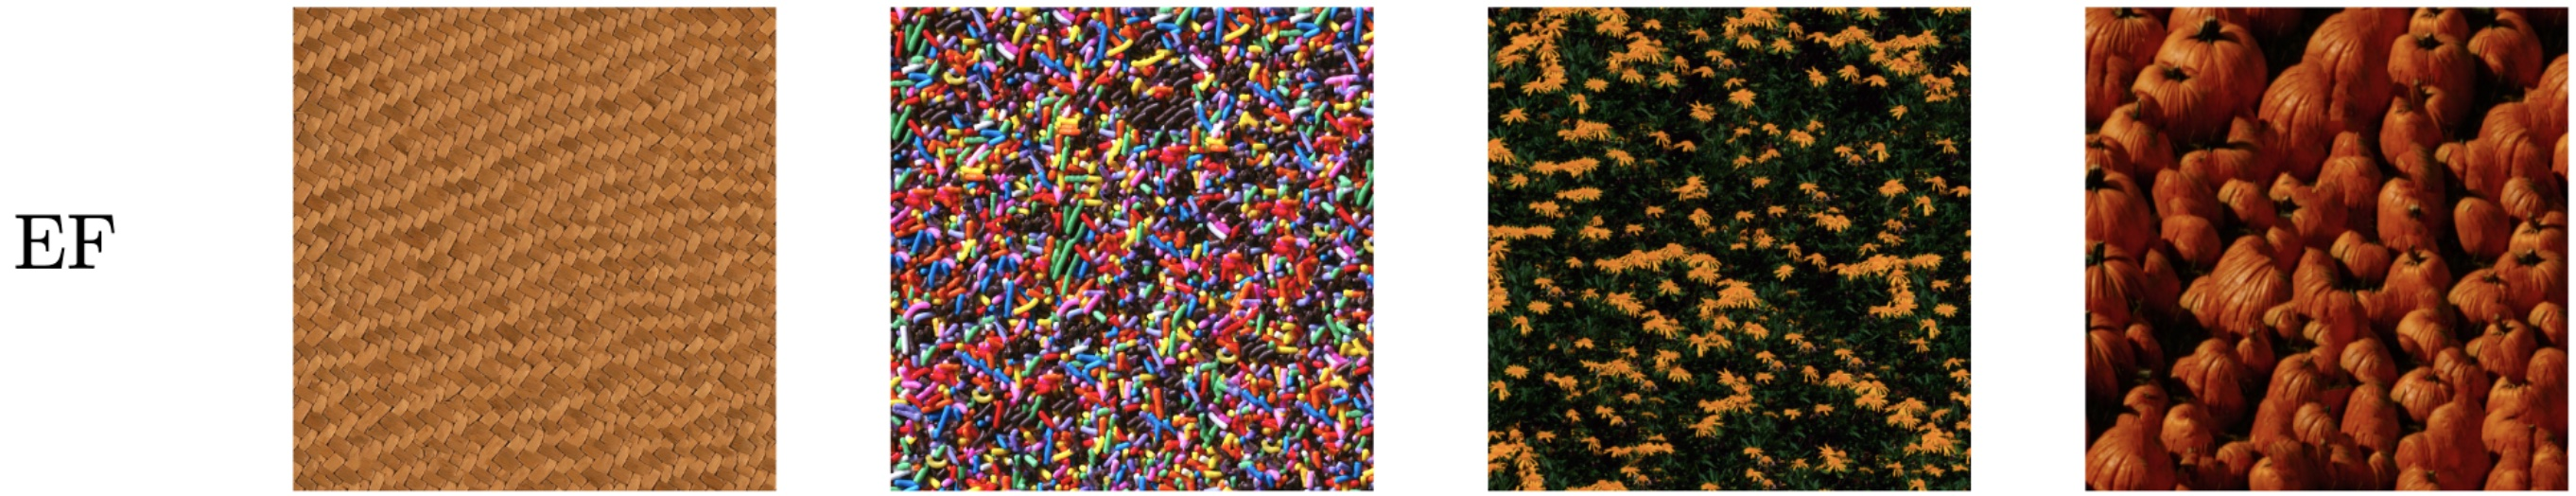
\includegraphics[width=\textwidth]{images/02-big_comparison_quilting_compressed.jpg}
        \caption*{}
        %\label{}
    \end{subfigure}

    \begin{subfigure}[b]{\textwidth}
        \centering
        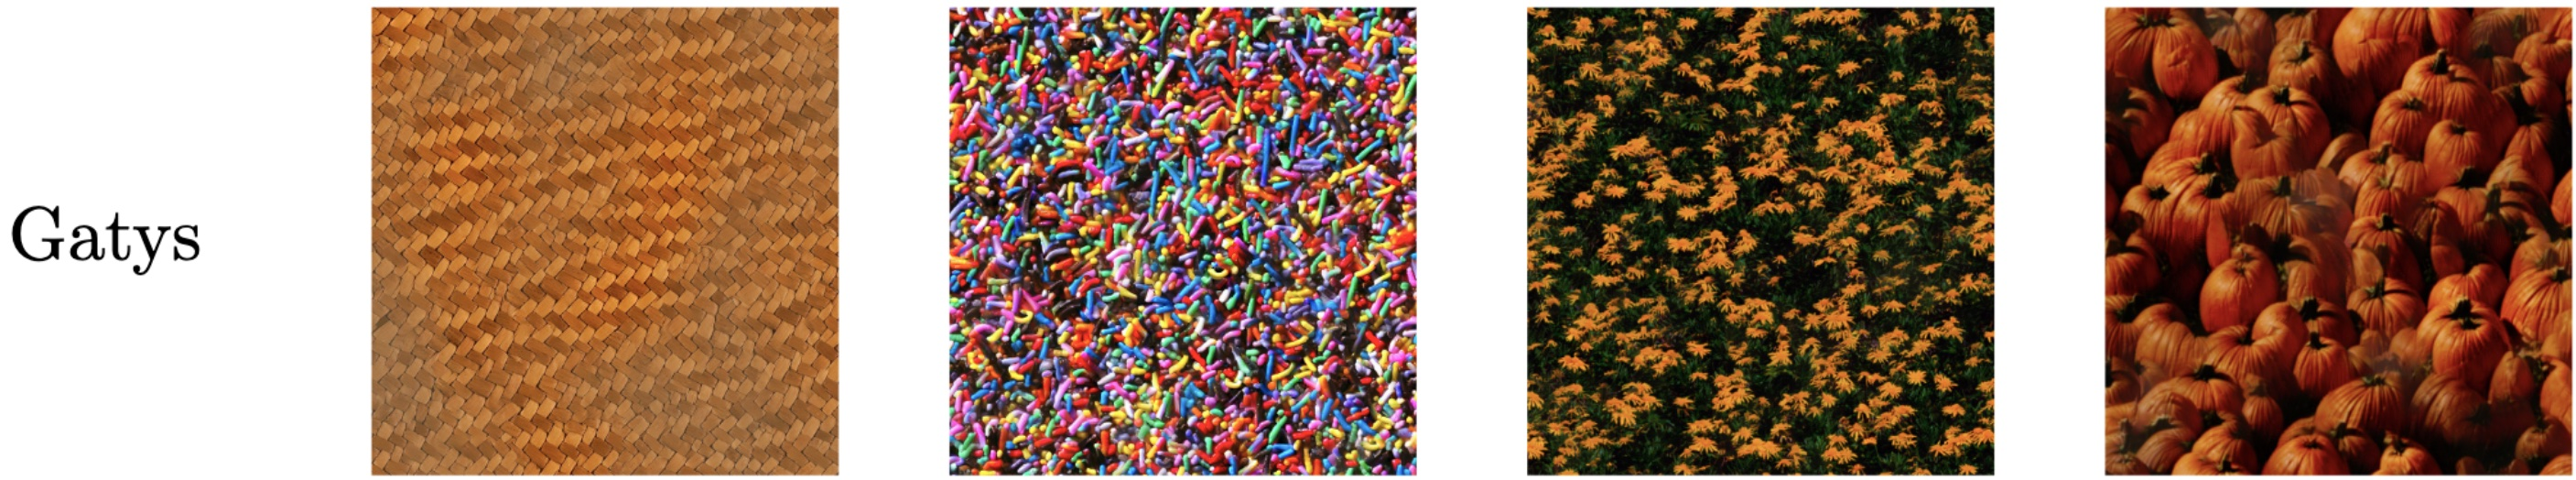
\includegraphics[width=\textwidth]{images/02-big_comparison_gatys_compressed.jpg}
        \caption*{}
        %\label{}
    \end{subfigure}
    \caption{A comparison of Gatys synthesis, Random Phase Noise (RPN, \citet{Galerne2011}) and image quilting (EF, \citet{Efros2001}). The chosen input textures are not very suitable for synthesis with Random Phase Noise as they contain fairly large features. Image quilting and Gatys seem to perform much better. Upon closer inspection, we can see that Gatys suffers from desaturated artifacts in the leftmost texture. Also, Gatys sometimes creates implausible shapes (e.g. deformed flower blooms). On the other hand, it is statistically closer to the input than EF (e.g. the flower texture generated by EF has too few blooms). Source: \citet{Raad2018}}
    \label{fig:background_synthesis_comparison}
\end{figure}

This method of synthesizing textures leads to high-quality results for a large variety of input images. Compared to patch-based synthesis it also provides a texture model, as opposed to a mere algorithm to generate new textures. This makes it easier to reason about and provide theoretical justifications as to why it works. Fig. \ref{fig:background_synthesis_comparison} taken from \citet{Raad2018} compares this method to others that we have discussed here and highlights their relative strengths and weaknesses.

\subsubsection{Potential Usage in Projection Mapping}
\label{section:background-texture_synthesis-statistics_based-projection_mapping}

This method can easily be adapted to projection mapping by modifying the optimization pipeline. The idea is to first project initial white noise image onto a scene using a differentiable rendering function. Then the resulting camera image would be fed into the CNN and ultimately compared against the input texture image. The loss gradients would flow through both the CNN and the rendering function to update the initial image. The result of this process would be an image would look like a new example of the input texture once projected.

\chapter{Methods}
\label{chapter:methods}

We now have all the building blocks needed to construct our method that implements projection mapping of textures by forcing the camera image to be a realization of the same texture as the desired appearance, instead of matching them pixel by pixel which is the usual approach (see Section~\ref{section:intro-key_idea} for more details on our key idea).

\begin{figure}[t]
    \centering
    \def\svgwidth{0.8\textwidth}
    \input{images/figures/03-system.pdf_tex}
    \caption{An overview of a complete projector-camera system. It receives desired appearance \(\bm{y}\) as input and outputs actual appearance \(r^\prime(\bm{p})\) by projecting a compensated projector image \(\bm{p}\) onto a given scene. Note that in order to perform the compensation, a function \(r\) which approximates \(r^\prime\) is needed. \(r\) is parameterized by information about the scene like geometry, materials and projector and camera properties. These parameters are marked LT and need to be provided by the projector and camera themselves via a calibration procedure. Texture source: \citet{Pixar128}}
    \label{fig:methods_system}
\end{figure}

We will first present an overview of our projection mapping pipeline and then focus on its main components.

\section{Pipeline Overview}
\label{section:methods-pipeline_overview}

\begin{figure}[]
    \centering
    \hspace*{-8mm}\makebox[\textwidth][c]{
        \def\svgwidth{1.1\textwidth}
        \input{images/figures/03-pipeline.pdf_tex}
    }\hspace*{8mm}
    \caption{An overview of our compensation pipeline with desired appearance \(\bm{y}\) as input and compensated projection image \(\bm{p}\) that minimizes eq.~\ref{eq:projection_mapping-statistics} as output. The upper part of the diagram is essentially a texture synthesis pipeline by \citet{Gatys2015}. The lower green part (the rendering function) is our extension that enables projection mapping. Instead of computing a set of statistics \(f\) on the synthesized image \(\bm{p}\) directly as \citet{Gatys2015} does, we first project \(\bm{p}\) to obtain \(r(\bm{p})\) and only then compute \(f\). The red projector symbol shows how \(\bm{p}\) is projected onto a mirror ball in our scene and the white scissors symbol shows how the camera image is cropped because we only want to match a portion of the scene. The whole process is an optimization loop with \(\bm{p}\) initialized to white noise and progressively refined until \(r(\bm{p})\) is a realization of the same texture as \(\bm{y}\) is. Texture source: \citet{Pixar128}}
    \label{fig:methods_pipeline}
\end{figure}

Projection mapping is typically done with a projector-camera system (see fig.~\ref{fig:intro_procam} for an example). Apart from the projector and the camera, such a system typically contains a software component which is responsible for compensating projection images via some kind of light transport modelling (see Section~\ref{section:background-projection_mapping-procams}). An illustration of what this looks like is shown in fig.~\ref{fig:methods_system}. However, we have decided to also simulate projector and camera virtually and thus create a complete software pipeline. The main reasons are the following:

\begin{itemize}
    \item A software implementation serves as necessary reference for future work. If something does not work in the controlled environment of a simulator, it will not work in the real world either
    \item Hardware systems come with challenges of its own, like signal-to-noise ratio, dynamic environment and time constraints. We want to focus on solving one challenge at a time, starting with projection quality
    \item Software pipelines are easier to modify and allow for rapid prototyping and experimentation
\end{itemize}

Note that as a consequence, we now use a light transport model both in the compensation component (function \(r\) in fig.~\ref{fig:methods_system}) and the projector-camera component (function \(r^\prime\) in fig.~\ref{fig:methods_system}).

Let us focus on the compensation pipeline first. Its goal is to minimize the expression in eq.~\ref{eq:projection_mapping-statistics}. The main input is an image \(\bm{y}\) which represents the desired appearance for our scene. Other inputs are the scene and projector (marked as LT in fig.~\ref{fig:methods_system}) which determine a rendering function \(r\) which creates a camera image \(r(\bm{p})\) out of a projector image \(\bm{p}\). A projector image \(\bm{p}\) which minimizes eq.~\ref{eq:projection_mapping-statistics} is the output of the pipeline. See fig.~\ref{fig:methods_pipeline} an illustration of how the pipeline works.

We build on top of a pipeline for texture synthesis used in \citet{Gatys2015} and extend it by the rendering function \(r\). The original synthesis pipeline is differentiable and relies on the gradient-based L-BFGS optimizer to synthesize a texture. Therefore, it is key that our \(r\) differentiable as well. This allows us to rely on L-BFGS to minimize eq.~\ref{eq:projection_mapping-statistics}.

In Section~\ref{section:background-texture_synthesis}, we have reviewed several texture synthesis methods that could potentially be used in our method. We have decided to use \citet{Gatys2015} over a patch-based method such as \citet{Efros2001} for the following reasons:

\begin{itemize}
    \item It achieves good results for a large variety of textures
    \item It defines a texture model which can be (and has been, as we will discuss later) improved to achieve better results while keeping the rest of the pipeline fixed
    \item It is very easy to adapt for projection mapping and does not impose any restrictions on the rendering function. In fact, a gradient-free version of the pipeline could theoretically be run on a physical projector-camera system
    \item Using an optimizer to gradually improve the result allows us to obtain a reasonable result quickly and improve it if more time is available
\end{itemize}

We will now describe the two main components of our compensation pipeline -- the rendering function \(r\) and the texture model which determines a set of statistics \(f(\bm{y})\) that fully describe a texture \(\bm{y}\) -- in more detail. We also focus on how the projector and camera are simulated and mention how our optimizer is configured.

\section{Rendering Function}
\label{section:methods-rendering_function}

The rendering function in our pipeline has the following form:

\begin{equation}
    \label{eq:rendering_function}
    r(\bm{p}, \phi) = \bm{y}  
\end{equation}

where \(\bm{p}\) is the projector image, \(\phi\) are scene parameters, such as geometry, materials, projector and camera position and orientation and so on. \(\bm{y}\) is the camera image whose statistics are matched against those of the input texture image (i.e. desired appearance). \(r\) needs to be differentiable because the statistics matching is done via gradient-based optimization.

\(r\) represents the act of projecting an image onto a scene and then capturing that projection. This is a fairly complex task, especially if the scene has arbitrary geometry, materials and external illumination. Luckily, in certain special scenarios, \(r\) can be very simple to formulate and fast to compute. We take advantage of this and use two different versions of \(r\) in our pipeline, a simple one to verify basic functionality and obtain reference results, and a general one to support arbitrary scenes.

\subsection{Simple Rendering Function}
\label{section:methods-rendering_function-simple}

Here is a scenario in which the light transport between the projector and the camera is easy to model:

\begin{itemize}
    \item The projector is pointed directly at a flat wall, with a right angle between its optical axis and the surface of the wall
    \item The surface of the wall is completely diffuse, meaning it looks matte and its appearance is not view-dependent
    \item The camera coincides with the projector
    \item We ignore light that is reflected from the wall into the rest of the scene and back into the camera
\end{itemize}

\begin{figure}[]
    \centering
    \def\svgwidth{0.6\textwidth}
    \input{images/figures/03-simple_scenario.pdf_tex}
    \caption{An illustration of the scenario modelled by the simple rendering function. The projector is pointed directly at the wall and coincides with the camera which allows for substantial simplification of the rendering process.}
    \label{fig:methods_simple_scenario}
\end{figure}

This scenario (see fig.~\ref{fig:methods_simple_scenario} for an illustration) is not too unrealistic -- it is a reasonable approximation of projecting onto a textured wall in a living room where the camera is right next to the projector and thus the projector-camera correspondence is straightforward to recover (as mentioned in Section~\ref{section:background-projection_mapping-procams-radiometric_calibration}, inter-reflection is minimal in this case and thus a 1:1 correspondence between projector and camera pixels can be assumed). See figs.~\ref{fig:intro_grossberg} and~\ref{fig:intro_result_teaser} for examples where such a scenario can be used.

Let us now derive a rendering function that handles this simple scenario directly from the rendering equation:

\begin{align}
    L(x \rightarrow \mathbf{v}) &= \int_{\Omega(x)} L(x \leftarrow \mathbf{u}) f_r(x, \mathbf{u} \rightarrow \mathbf{v}) \cos \theta \mathrm{d}\mathbf{u} + E(x \rightarrow \mathbf{v}) \label{eq:simple_x_from_rendering_eq01} \\
    &= \int_{\Omega(x)} L(x \leftarrow \mathbf{u}) f_r(x, \mathbf{u} \rightarrow \mathbf{v}) \cos \theta \mathrm{d}\mathbf{u} \label{eq:simple_x_from_rendering_eq02} \\
    &= \int_{\Omega(x)} L(x \leftarrow \mathbf{u}) \rho \frac{\cos \theta}{\pi} \mathrm{d}\mathbf{u} \label{eq:simple_x_from_rendering_eq03} \\
    &= \int_{\Omega(x)} E(x \leftarrow \mathbf{u}) \rho \frac{\cos \theta}{\pi} \mathrm{d}\mathbf{u} \label{eq:simple_x_from_rendering_eq04} \\
    &\approx E(x \leftarrow \mathbf{-v}) \rho \frac{\cos \theta}{\pi r^2} \label{eq:simple_x_from_rendering_eq05}
\end{align}

Eq.~\ref{eq:simple_x_from_rendering_eq01} is the rendering equation. We move to eq.~\ref{eq:simple_x_from_rendering_eq02} by observing that our background is not an emitter in itself. Eq.~\ref{eq:simple_x_from_rendering_eq03} is obtained by assigning the diffuse BRDF function \(\rho / \pi\) to the background surface. \(\rho\) is surface albedo which corresponds to the value of the background image at \(x\). \(\pi\) is a scaling constant needed to preserve energy in the scene. Eq.~\ref{eq:simple_x_from_rendering_eq04} comes from our assumption that the only radiance that arrives at point \(x\) on the background comes from the projector. Finally, the integral can be approximated (eq.~\ref{eq:simple_x_from_rendering_eq05}) by restricting the area we integrate over to the solid angle subtended by a projector pixel, assuming the integrand is constant over that area and setting \(u = v\). The area is inversely proportional to the square of the distance between the projector pixel and \(x\). Finally, we observe that \(E(x \leftarrow \mathbf{-v})\) is a value in \(\bm{p}\) and \(\rho\) is a value in the background image.

This leads us to the following straightforward and differentiable rendering function \(r\):

\begin{equation}
    \label{eq:rendering_function-simple}
    r(\bm{p}, \bm{b}) = c \cdot \bm{p} \cdot \bm{b} = \bm{y}
\end{equation}

where \(\bm{p}\) and \(\bm{y}\) are again the projector and camera image, respectively, \(\bm{b}\) is the background -- an image (texture) representing the surface of the wall -- and \(c\) is a constant that roughly accounts for \(\cos \theta / \pi r^2\). Here is where we perform the last simplification. \(r\) and \(\theta\) vary over the background and depend on how far the projector is from the background. However, we are only interested in simulating situations where the projector cannot be bright enough to compensate the projection with conventional methods but where it is still capable of compensating with our method. We thus set \(r\) ourselves to adjust the distance and the brightness of the projector according to our needs as part of a single constant \(c\). The variation of \(\cos \theta\) can be accounted for after the fact by darkening \(\bm{p}\) towards the center. This means that we also have to assume that the minimum brightness of our projector is not limited by the scenario.

To summarize, the simple rendering function \(r\) can be very easily integrated into Gatys' synthesis pipeline and represents negligible computational overhead. This allows for rapid experimentation that yields reference results for a reasonable subset of projection scenarios. However, a more general solution for projection mapping on arbitrary 3D scenes is also needed. We cover it in the next section.

\subsection{General Scenario}
\label{section:methods-rendering_function-general}

A possible candidate for a general rendering function that computes camera images from projector image for arbitrary 3D scenes is simply a renderer such as PBRT (\citet{PBRT3e}) or Mitsuba (\citet{Mitsuba}). These renderers are programs that accept a scene configuration file as input and output an image of the scene as seen from the point of view of a virtual camera. For example, fig.~\ref{fig:background_linear_lt} was created using Mitsuba. Renderers often implement a large variety of materials, camera effect, rendering equation solvers and other features that make them incredibly versatile. And indeed, they match the signature of our rendering function well:

\begin{equation}
    \label{eq:rendering_function-renderer}
    r(\bm{p}, \textit{config}) = \bm{y}
\end{equation}

where \(r\) is the renderer and \textit{config} represents the configuration file which also describes how the projector image \(\bm{p}\) is used in the scene. However, renderers come with two main caveats:

\begin{itemize}
    \item They are generally not differentiable
    \item They require a complete description of scene geometry and materials which is rarely available in a projection mapping application
\end{itemize}

Both points are nowadays being addressed by differentiable renderers such as Mitsuba 2 (\citet{Mitsuba2}), but these systems are general-purpose and therefore too computationally heavy to be used in a texture synthesis pipeline. Instead, we use the fact that light transport in an arbitrary scene is linear and model our general rendering function \(r\) with a light transport matrix that was described in Section~\ref{section:background-projection_mapping-procams-inverse_lt}:

\begin{equation}
    \label{eq:rendering_function-lt_matrix}
    r(\bm{p}, A) = c \cdot A\bm{p} = \bm{y}
\end{equation}

where \(A\) is the light transport matrix (see~\ref{eq:lt_matrix}) and \(\bm{p}\) is supposed to be a vector representing the light sources in the scene. But this is exactly our projector image where each pixel corresponds to a light source that we can control separately. \(c\) is the same multiplier as in eq.~\ref{eq:rendering_function-simple} whose purpose is to tune the overall brightness of the projector.

Multiplication by large matrices is differentiable, very fast on modern GPUs and the matrix size (and thus the computation time) depends only on the resolution of the projector and camera images, not on scene complexity. This makes them easy to use in a texture synthesis pipeline. However, the process of acquiring them is not entirely straightforward. We focus on it in the next section.

\subsubsection{Capturing the Light Transport Matrix}
\label{section:methods-rendering_function-general-lt_capture}

If a scene contains two lamps as light sources, then capturing a light transport matrix with respect to those lamps is nothing more than taking two photographs of the scene -- one for each lamp switched on separately. Our scene contains as many lamps as there are pixels in our projector image \(\bm{p}\) (we can ignore other light sources because those are fixed). Taking a photograph for each of the projector pixels being switched on separately is practically impossible because of the signal-to-noise ratio of cameras -- no camera is able to capture such tiny signal as that coming from a single projector pixel.

If the goal is to capture an LT matrix of a real scene using a camera, there are other ways of doing it. Capturing one projector pixel at a time corresponds to capturing the canonical basis of the matrix (see fig.~\ref{fig:background_lt_capture} for an illustration). As we saw in Section~\ref{section:background-projection_mapping-procams-inverse_lt}, better bases that comprise brighter patterns can be used to ease the capture process. The fact that the matrix is often very sparse can also be used.

However, our projector-camera system is simulated fully in software which means that our scenes are virtual and we know precisely which geometry and materials they contain. We can thus capture the canonical basis directly using a renderer whose floating-point arithmetic can handle tiny signals. We use Mitsuba to render camera images of our scene illuminated by each projector pixel separately and then assemble the images into the LT matrix \(A\). Note that the LT matrix capture process is the main part of our pipeline which would usually be done by a physical projector and camera but which we simulate. The rest of the pipeline could work just as well in a physical projector-camera system where the LT matrix \(A\) would be captured from a real scene. See fig.~\ref{fig:methods_system} for an illustration.

We now describe the capture process in more detail, focusing on how to configure Mitsuba for our purposes and how to work with the LT matrix. Specifically, we look at three topics:

\begin{itemize}
    \item How to implement a projector in Mitsuba?
    \item How to solve the rendering equation efficiently with only a single active projector pixel?
    \item How large is the light transport matrix and what are the implications?
\end{itemize}

\textbf{How to implement a projector in Mitsuba?} Our requirements for the virtual projector are reasonably good-looking projections where the basic limitations we wish to overcome are present: limited gamut and depth of field. The Mitsuba renderer has very rudimentary projector functionality in the form of a spotlight with a projective texture (see fig.~\ref{fig:methods_projector_features_spotlight}). This is not enough for our purposes because it creates only circular projections and lacks depth of field. We have thus decided to add the following two features to Mitsuba's projector implementation:

\begin{itemize}
    \item Rectangular projection frustum (see fig.~\ref{fig:methods_projector_features_frustum})
    \item Thin lens optics (see fig.~\ref{fig:methods_projector_features_thin_lens})
\end{itemize}

Rectangular projection frustum is necessary because we want to project rectagular images. The thin lens model (described in Section~\ref{section:background-projection_mapping-projectors-dof}) allows us to simulate the depth of field effect with sufficient accuracy. We focus on the upper limit of projector gamut by simply restricting the values of projector image \(\bm{p}\) to \([0, 1]\) and a suitable choice of multiplier \(c\) (see eq.~\ref{eq:rendering_function-lt_matrix}).

\begin{figure}[]
    \centering
    \begin{subfigure}[b]{0.32\textwidth}
        \centering
        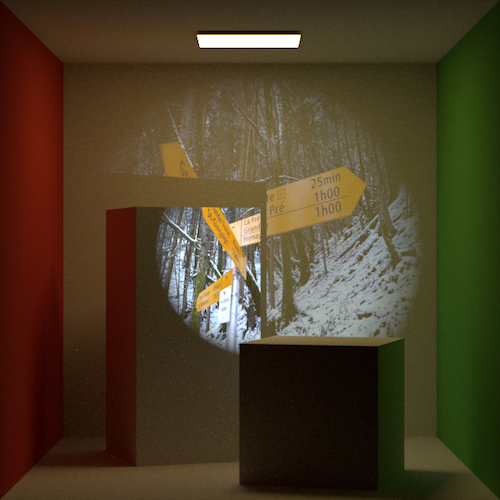
\includegraphics[width=\textwidth]{images/03-projector_features-spotlight.jpg}
        \caption{Original Mitsuba projector}
        \label{fig:methods_projector_features_spotlight}
    \end{subfigure}
    \hfill
    \begin{subfigure}[b]{0.32\textwidth}
        \centering
        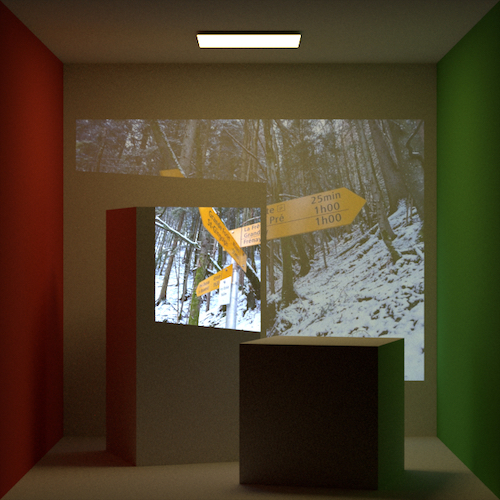
\includegraphics[width=\textwidth]{images/03-projector_features-frustum.jpg}
        \caption{Added rectangular projection frustum}
        \label{fig:methods_projector_features_frustum}
    \end{subfigure}
    \hfill
    \begin{subfigure}[b]{0.32\textwidth}
        \centering
        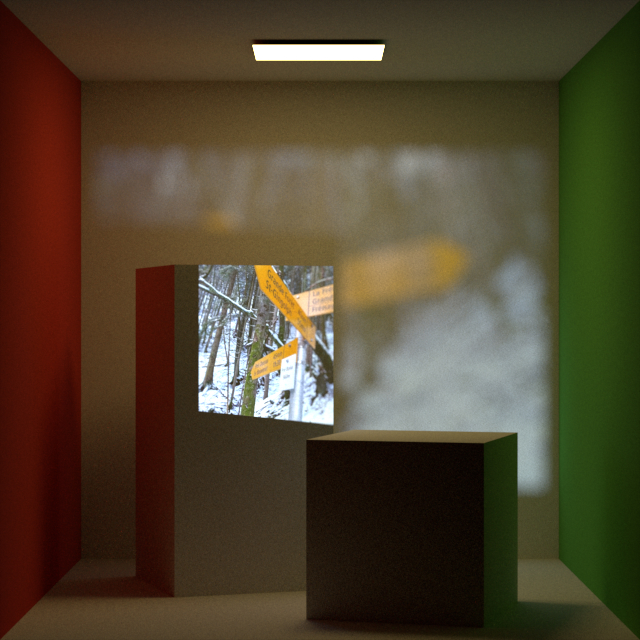
\includegraphics[width=\textwidth]{images/03-projector_features-thin_lens.jpg}
        \caption{Added thin lens model}
        \vspace*{5mm}
        \label{fig:methods_projector_features_thin_lens}
    \end{subfigure}
    \caption{Projector features that we have implemented in Mitsuba to support the needs of our projection mapping pipeline. Image~(a) shows  a spotlight with a projective texture that Mitsuba already supported but was not sufficient for us. Image~(b) shows a rectangular projection frustum that we have added to support rectangular projections. Image~(c) shows our final projector implementation with a thin lens optics model that enables the depth of field effect}
    \label{fig:methods_projector_features}
\end{figure}

\textbf{How to solve the rendering equation efficiently with only a single active projector pixel?} Projecting images with our custom projector implementation yields good results (see fig.~\ref{fig:methods_projector_features_thin_lens}). However, in order to capture the light transport matrix, we need to project images with only a single active pixel. And this turns out to be problematic due to the way the rendering equation (\ref{eq:rendering_equation}) is typically solved. A \textit{path tracer} (PT), which is the default Monte Carlo solver in Mitsuba and most other renderers, samples random paths from camera, computes radiance travelling along them in the opposite direction and builds an estimate of the final image. In our case, this means that a random walk from the camera needs to sample a single pixel on the projector to yield a light-carrying path. The probability of this happening is extremely low and most paths thus do not contribute anything to the estimate. This results in poor convergence and extremely long rendering time. See fig.~\ref{fig:methods_sampling_path} for an example.

However, while some path sampling techniques build path starting from the camera, others start from the emitter. When emitters are very small, like points lights or projectors with only a single white pixel, it is important to start building the path from the light. We therefore use the bi-directional path tracing (BDPT) algorithm which combines paths that start both from the camera and from emitters and which is already implemented in Mitsuba. More on BDPT can be found in \citet{Veach1997}. See fig.~\ref{fig:methods_sampling_bdpt} for an example.

Another issue is with sampling a point on the projector where a path could start from. If uniform sampling is used, the only active pixel would be sampled in 1 out of \(m \cdot n\) samples on average where \(m\) and \(n\) are the dimensions of \(\bm{p}\). This would again yield many paths with zero contribution. To fix this, we have implemented a common variance reduction technique technique used in Monte Carlo integration called \textit{importance sampling}. Importance sampling chooses samples with larger contribution with higher probability. In our case, we base the probability of choosing a projector pixel on the relative contribution of the pixel to the brightness of the whole projector image. This means that when capturing the canonical basis of an LT matrix, the only active pixel is sampled with probability 1 and other pixels are not sampled at all. See fig.~\ref{fig:methods_sampling_bdpt_importance} for an example.

\begin{figure}[ht]
    \centering
    \begin{subfigure}[b]{0.32\textwidth}
        \centering
        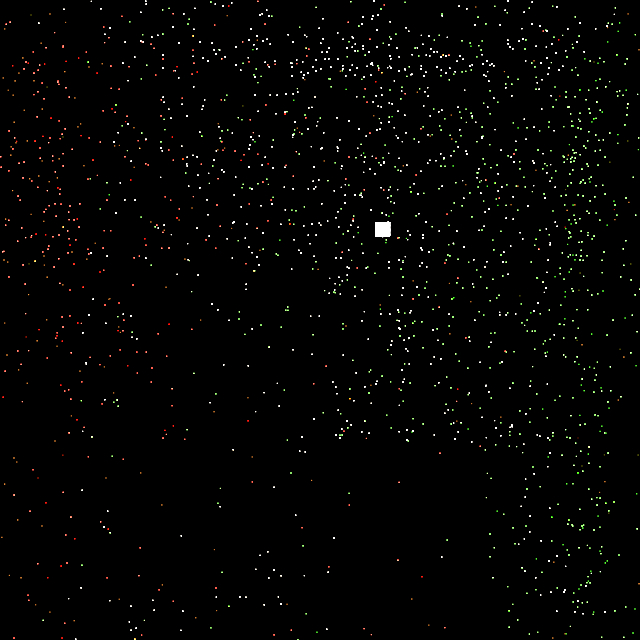
\includegraphics[width=\textwidth]{images/03-sampling_path.jpg}
        \caption{Path tracer}
        \vspace*{5mm}
        \label{fig:methods_sampling_path}
    \end{subfigure}
    \hfill
    \begin{subfigure}[b]{0.32\textwidth}
        \centering
        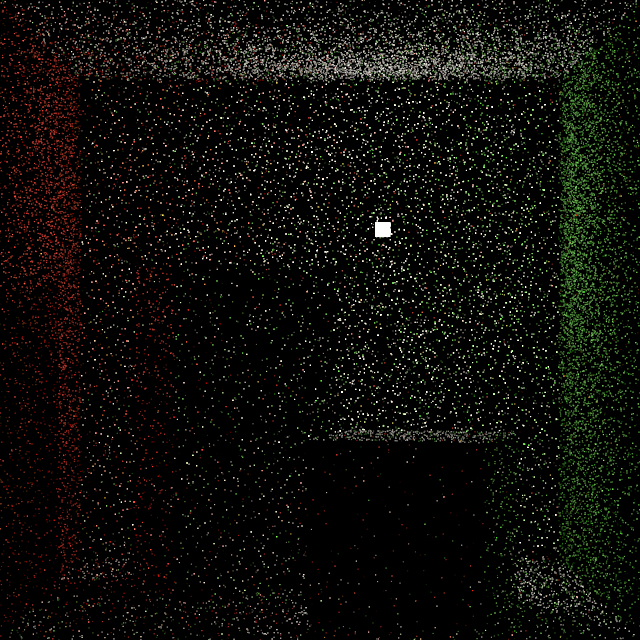
\includegraphics[width=\textwidth]{images/03-sampling_bdpt.jpg}
        \caption{BDPT}
        \vspace*{5mm}
        \label{fig:methods_sampling_bdpt}
    \end{subfigure}
    \hfill
    \begin{subfigure}[b]{0.32\textwidth}
        \centering
        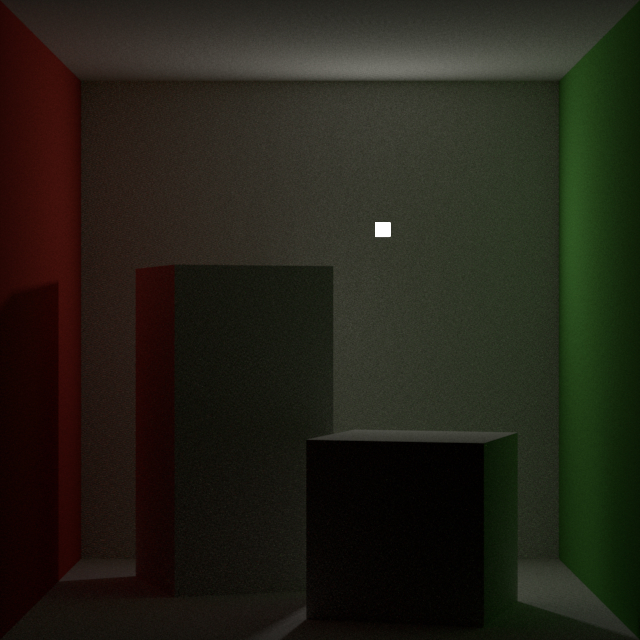
\includegraphics[width=\textwidth]{images/03-sampling_bdpt_importance.jpg}
        \caption{BDPT with importance sampling}
        \label{fig:methods_sampling_bdpt_importance}
    \end{subfigure}
    \caption{A comparison of various sampling techniques to solve the rendering equation. The scene is being projected onto by a \(640 \times 480\) image with only a small \(20 \times 20\) patch of active pixels. All images were rendered using 16 path samples per pixel. Image~(a) shows a basic path tracer which samples random light-carrying paths starting from the camera. Image~(b) is bi-directional path tracing (BDPT), a better technique which combines paths from both camera and light sources. Image~(c) shows BDPT with importance sampling of the projector image which greatly reduces noise. This is the method we use in our pipeline.}
    \label{fig:methods_sampling}
\end{figure}

\textbf{How large is the light transport matrix and what are the implications?} The last practical consideration we need to make is about the size of the light transport matrix. Here is how it is determined:

\begin{equation}
    \label{eq:lt_matrix_size}
    S = p_w \cdot p_h \cdot c_w \cdot c_h \cdot 3 \cdot 4
\end{equation}

where \(S\) is the matrix size in bytes, \(p_w\) and \(p_h\) is the width and height of the projector image, respectively, \(c_w\) and \(c_h\) are the dimensions of the camera image. We then assume three color channels and four bytes to store each intensity value. It is important to store the intensity values as 32-bit floating point numbers to capture the tiny signal coming from individual projector pixels. See an example of how value precision influences the noise level of basis images in fig.~\ref{fig:methods_float}.

This means that an LT matrix for projector and camera image of size \(160 \times 160\) is over 7.8 GB large. This is the size we have used in our experiments because it is sufficient to demonstrate the performance of our method and because it fit well into the memory of our GPUs. However, it is clear that this approach to implementing the rendering function is not very scalable. For our purposes, this approach has the advantage of being simple and accurate which is important when evaluating the basic functionality of a new method. For practical use, more data-efficient methods like those mentioned in Section~\ref{section:background-projection_mapping-procams-inverse_lt} are needed.

\begin{figure}[]
    \centering
    \begin{subfigure}[b]{0.48\textwidth}
        \centering
        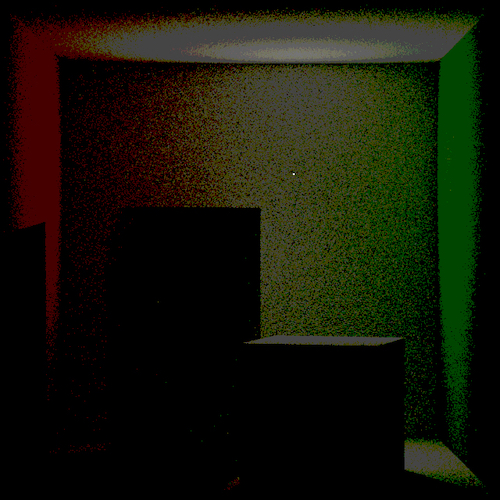
\includegraphics[width=\textwidth]{images/03-floating_point16.jpg}
        \caption{16-bit float}
        \label{fig:methods_float16}
    \end{subfigure}
    \hfill
    \begin{subfigure}[b]{0.48\textwidth}
        \centering
        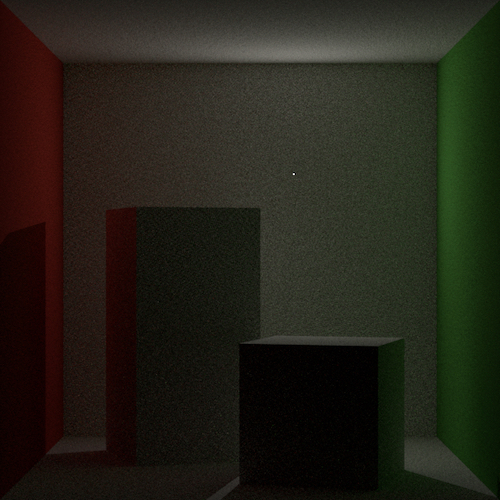
\includegraphics[width=\textwidth]{images/03-floating_point32.jpg}
        \caption{32-bit float}
        \label{fig:methods_float32}
    \end{subfigure}
    \caption{An illustration of how pixel value precision influences noise level in basis images. The scene is illuminated by a \(640 \times 480\) projection image where only a single pixel is active. The resulting images are scaled by \(10^6\) for visualization purposes. Image~(a) is stored in 16-bit floating point, while image~(b) is stored in 32-bit floating point}
    \label{fig:methods_float}
\end{figure}

This concludes the section on our rendering function \(r\). In the following section we cover the second building block of our projection mapping pipeline, the texture model \(f\).

\section{Texture Model}
\label{section:methods-texture_model}

Our texture model is built on top of that used in \citet{Gatys2015} and described in Section~\ref{section:background-texture_synthesis-statistics_based-synthesis_using_cnns}. While the vanilla Gatys model achieves very good results, it also has several shortcomings, such as desaturated patches when synthesizing textures larger than input or physically implausible feature deformation (see figs.~\ref{fig:methods_comparison_small-vanilla} and~\ref{fig:methods_comparison_large-vanilla} for examples).

These shortcomings are well known and have been studied by several authors who have introduced improvements to the original model which result in higher quality texture synthesis. It is unclear, however, whether improvements in texture synthesis also translate into improvements in the projection mapping of textures. We have thus decided to reimplement the original Gatys model along with the improvements and evaluate how each of them peforms in our setup.

\citet{Gatys2015} have provided an implementation of their algorithm in the Caffe (\citet{Jia2014}) deep learning framework. Because this framework is not very commonly used anymore (last stable version was released in 2017, according to \citet{CaffeGitHub}), we have ported the algorithm to PyTorch which is currently more actively maintained and therefore easier to work with.

\subsection{Improving Gatys Texture Synthesis}
\label{section:methods-texture_model-improvements}

As discussed in Section~\ref{section:background-texture_synthesis-statistics_based-synthesis_using_cnns}, the original Gatys algorithm synthesizes a texture \(\bm{y_2}\) from an example \(\bm{y_1}\) by minimizing the difference between their statistics \(f(\bm{y_2})\) and \(f(\bm{y_1})\) which fully describe a texture under the Gatys texture model. The specific form of \(f\) determines the performance of the synthesis algorithm.

We have implemented three different improvements to the original Gatys statistics. In general, all of them tend to reduce the ambiguity of the texture description (i.e. reduce the size of texture classes as defined by their texture model) and thus better enforce texture structure while maintaining high variance of reasonable outputs. We now briefly describe each of the three improvements.

\subsubsection{Activation Shift}
\label{section:methods-texture_model-improvements-activation_shift}

In the original Gatys model, a set Gram matrices of VGG-19 layer activations form the set of descriptive statistics \(f\):

\begin{equation}
    \label{eq:gatys_statistics}
    f(\bm{y}) = \{G^1(\bm{y}), \dots, G^L(\bm{y})\}
\end{equation}

where \(L\) is a chosen number of VGG-19 layers that are used for synthesis and a Gram matrix \(G^l(\bm{y})\) is defined as

\begin{equation}
    \label{eq:gram_style}
    G_{ij}^l(\bm{y}) = \sum_k F_{ik}^l(\bm{y}) F_{jk}^l(\bm{y})
\end{equation}

where \(i\) and \(j\) are filters in layer \(l\) and \(F_{jk}^l\) is the activation of the \(j\)-th filter at position \(k\) in layer \(l\). A Gram matrix thus represents the correlations between feature reponses in a network layer.

\citet{Novak2016} have introduced a number of simple improvements to the way Gram matrices are calculated from VGG-19 activations. One of them is called \textit{activation shift}. In the original Gatys model, activations \(F_{jk}^l\) are non-negative with mean 1. Also, the resulting Gram matrices \(G^l\) tend to be very sparse with many zero entries. \citet{Novak2016} argue that these zero entries are a source of ambiguity in texture description because they could have many causes:

\begin{itemize}
    \item Both features that the activations represent are missing from the image
    \item Only one of the features is present
    \item Both of them are present but never appear together
\end{itemize}

To remove this ambiguity, \citet{Novak2016} suggest to offset the activations by \(-1\) before computing the Gram matrices:

\begin{equation}
    \label{eq:gram_style_activation_shift}
    G_{ij}^l = \sum_k (F_{ik}^l - 1) (F_{jk}^l - 1)
\end{equation}

This is extremely simple to implement and brings clear improvements to synthesis quality (see figs.~\ref{fig:methods_comparison_small-shift} and~\ref{fig:methods_comparison_large-shift}).

\subsubsection{Correlation Chain}
\label{section:methods-texture_model-improvements-correlation_chain}

\citet{Novak2016} present one more useful modification to Gram matrix computation. In the original algorithm, only activations from the same layer are correlated with each other to form a Gram matrix. \citet{Novak2016} suggest to correlate activations from neighbouring layers as well. Because activation maps \(F^l\) and \(F^k\) where \(l\) and \(k\) are neighbouring layers may have different dimensions, the smaller map needs to be upsampled first. As a result a new set of matrices \(G^{lk}\) is added to the original set \(G^l\) to further lower the ambiguity of the texture description:

\begin{equation}
    \label{eq:gram_style_chain}
    G^{lk} = F^l [\textit{up}(F^k)]^T
\end{equation}

where \(l = 1 \dots L - 1\), \(L\) is the number of chosen layers, \(k = l + 1\) and \textit{up} is an upsampling procedure. The contribution of this modification to texture synthesis can be seen in figs.~\ref{fig:methods_comparison_small-chain} and~\ref{fig:methods_comparison_large-chain}.

\subsubsection{Gaussian Pyramid}
\label{section:methods-texture_model-improvements-gaussian_pyramid}

\citet{Snelgrove2017} has observed that the performance of Gatys synthesis is greatly limited by the receptive fields of the underlying VGG-19 network. The network was trained on images of size \(224 \times 224\) and its capability to capture information about large features is larger images is thus limited (see~\ref{fig:methods_receptive_field} for an illustration).

\begin{figure}[ht]
    \centering
    \begin{subfigure}[b]{0.48\textwidth}
        \centering
        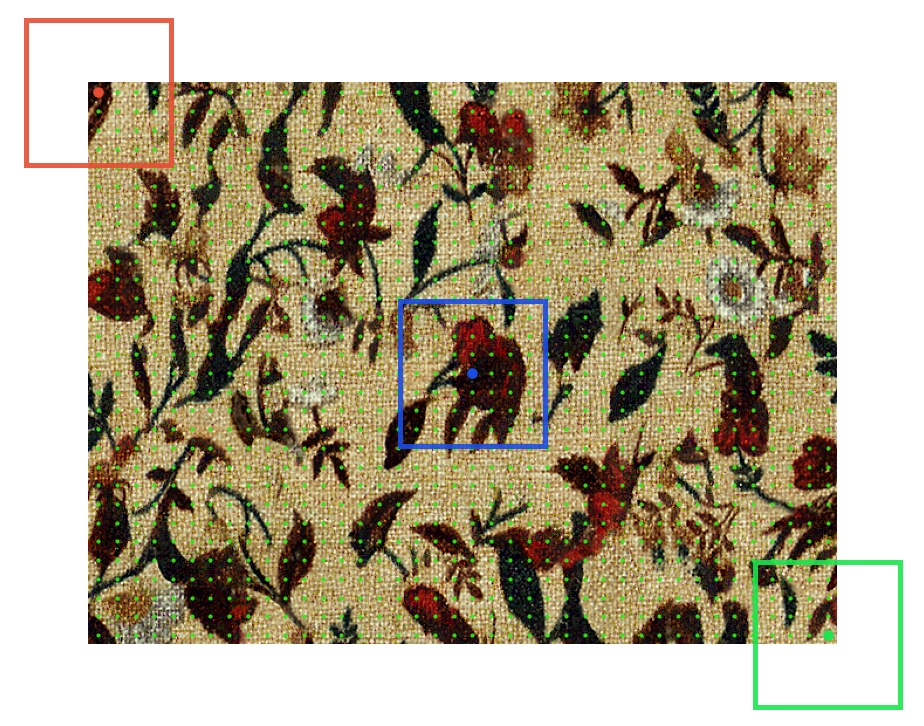
\includegraphics[width=\textwidth]{images/03-receptive_field-level0.jpg}
        \caption{VGG-19 receptive fields on a \(640 \times 480\) image}
        \label{fig:methods_receptive_field_lvl0}
    \end{subfigure}
    \hfill
    \begin{subfigure}[b]{0.48\textwidth}
        \centering
        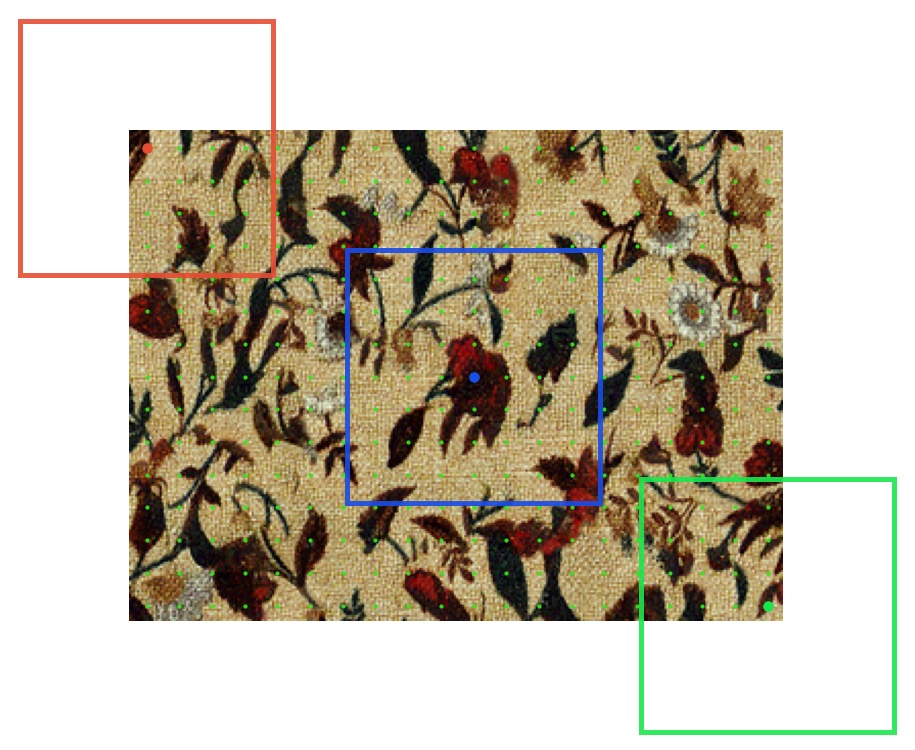
\includegraphics[width=\textwidth]{images/03-receptive_field-level1.jpg}
        \caption{VGG-19 receptive fields on a \(320 \times 240\) image}
        \label{fig:methods_receptive_field_lvl1}
    \end{subfigure}
    \caption{A comparison of the receptive fields (depicted as colorful squares) of the last convolutional layer of VGG-19 used in the Gatys texture model. A receptive field of a network layer activation is essentially a patch of pixels of the input image which has an effect on that particular activation (recall fig.~\ref{fig:background_cnn}). If a texture feature is larger than the receptive field of a given activation, then it cannot be captured by statistics computed on the activation. Figure~(a) uses an input image of size \(640 \times 480\) while figure~(b) uses size \(320 \times 240\). Texture source: \citet{Pixar128}}
    \label{fig:methods_receptive_field}
\end{figure}

To fix this, he proposes to not compute the Gram matrices on images, but rather on Gaussian pyramids of images. This means that instead of eq.~\ref{eq:gatys_statistics}, he uses

\begin{equation}
    \label{eq:snelgrove_statistics}
    f(\bm{y}) = \{\{G^1(\bm{y_i}) | i = 1, \dots, s\}, \dots, \{G^L(\bm{y_i}) | i = 1, \dots, s\}\}
\end{equation}

where \(\bm{y_i}\) is image \(\bm{y_{i - 1}}\) downsampled by half using proper pre-filtering, such as Lanczos. \(s\) is a chosen number of scales which depends on the size of the texture we wish to synthesize. As a result, even more Gram matrices are used to further disambiguate the texture description. Results of this modification can be seen in figs.~\ref{fig:methods_comparison_small-pyramid} and~\ref{fig:methods_comparison_large-pyramid}.

\begin{figure}[ht]
    \centering    
    \begin{subfigure}{0.8\textwidth}
        \centering
        \begin{subfigure}{0.32\textwidth}
            \centering
            \begin{tikzpicture}
                \draw (0, 0) node[inner sep=0] {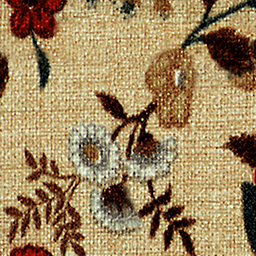
\includegraphics[width=\textwidth]{images/03-comparison_small_target.jpg}};
                \fill[black] (-1.7, 1.2) rectangle ++(2.2, 0.5);
                \node [anchor=center] at (-0.6, 1.42) {{\color{white} \(256 \times 256\)}};
                \draw[line width=0.8mm, black] (-1.75, -1.75) rectangle ++(3.5, 3.5);
            \end{tikzpicture}
            \caption{\textbf{Input}}
            \label{fig:methods_comparison_small-target}
        \end{subfigure}
        \hfill
        \begin{subfigure}{0.32\textwidth}
            \centering
            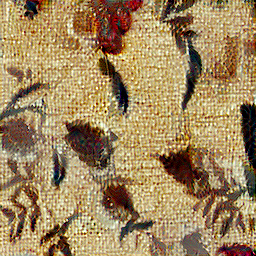
\includegraphics[width=\textwidth]{images/03-comparison_small_vanilla.jpg}
            \caption{Gatys}
            \label{fig:methods_comparison_small-vanilla}
        \end{subfigure}
        \hfill
        \begin{subfigure}{0.32\textwidth}
            \centering
            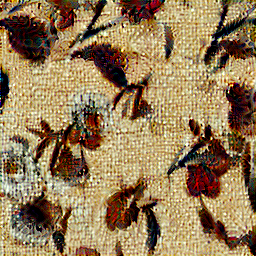
\includegraphics[width=\textwidth]{images/03-comparison_small_shift.jpg}
            \caption{Shift}
            \label{fig:methods_comparison_small-shift}
        \end{subfigure}
        
        \begin{subfigure}{0.32\textwidth}
            \centering
            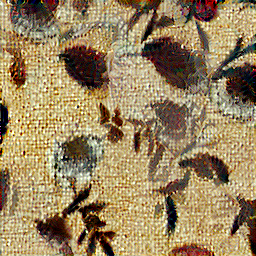
\includegraphics[width=\textwidth]{images/03-comparison_small_chain.jpg}
            \caption{Chain}
            \label{fig:methods_comparison_small-chain}
        \end{subfigure}
        \hfill
        \begin{subfigure}{0.32\textwidth}
            \centering
            \includegraphics[width=\textwidth]{images/03-comparison_small_pyramid.jpg}
            \caption{Pyramid}
            \label{fig:methods_comparison_small-pyramid}
        \end{subfigure}
        \hfill
        \begin{subfigure}{0.32\textwidth}
            \centering
            \includegraphics[width=\textwidth]{images/03-comparison_small_pyramid_shift.jpg}
            \caption{Pyramid + Shift}
            \label{fig:methods_comparison_small-pyramid_shift}
        \end{subfigure}
        \vskip 20pt
        % -------------------------------------------
        \begin{subfigure}{0.32\textwidth}
            \centering
            \begin{tikzpicture}
                \draw (0, 0) node[inner sep=0] {\includegraphics[width=\textwidth]{images/03-comparison_large_target.jpg}};
                \fill[black] (-1.7, 1.2) rectangle ++(2.2, 0.5);
                \node [anchor=center] at (-0.6, 1.42) {{\color{white} \(512 \times 512\)}};
                \draw[line width=0.8mm, black] (-1.75, -1.75) rectangle ++(3.5, 3.5);
            \end{tikzpicture}
            \caption{\textbf{Input}}
            \label{fig:methods_comparison_large-target}
        \end{subfigure}
        \begin{subfigure}{0.32\textwidth}
            \centering
            \includegraphics[width=\textwidth]{images/03-comparison_large_vanilla.jpg}
            \caption{Gatys}
            \label{fig:methods_comparison_large-vanilla}
        \end{subfigure}
        \hfill
        \begin{subfigure}{0.32\textwidth}
            \centering
            \includegraphics[width=\textwidth]{images/03-comparison_large_shift.jpg}
            \caption{Shift}
            \label{fig:methods_comparison_large-shift}
        \end{subfigure}
        
        \begin{subfigure}{0.32\textwidth}
            \centering
            \includegraphics[width=\textwidth]{images/03-comparison_large_chain.jpg}
            \caption{Chain}
            \label{fig:methods_comparison_large-chain}
        \end{subfigure}
        \hfill
        \begin{subfigure}{0.32\textwidth}
            \centering
            \includegraphics[width=\textwidth]{images/03-comparison_large_pyramid.jpg}
            \caption{Pyramid}
            \label{fig:methods_comparison_large-pyramid}
        \end{subfigure}
        \hfill
        \begin{subfigure}{0.32\textwidth}
            \centering
            \includegraphics[width=\textwidth]{images/03-comparison_large_pyramid_shift.jpg}
            \caption{Pyramid + Shift}
            \label{fig:methods_comparison_large-pyramid_shift}
        \end{subfigure}
    \end{subfigure}
    \caption{A comparison of texture synthesis under various models described in this section. The goal is to generate a new example of the input texture. The upper two rows contain images of size \(256 \times 256\) while the lower two rows contain images of size \(512 \times 512\). Note desaturated patches and inaccurate colors when Shift is not used and large feature distortion under the Gatys texture model. Lastly, note that Pyramid describes the small texture so accurately that it synthesizes an image nearly identical to the input. Texture source: \citet{Pixar128}}
    \label{fig:methods_comparison_small}
\end{figure}

\section{Optimization Details}
\label{section:methods-optimization}

In eq.~\ref{eq:projection_mapping-limitations}, we have formally expressed that projections cannot be arbitrarily bright nor arbitrarily dark because there are limits set by both the projector gamut and the scene. However, our pipeline as we have described it thus far does not take this into account because we have no restrictions on what the values of \(\bm{p}\) can be. Let us now briefly discuss how we treat this issue in our pipeline.

The first observation we make is that in our model, the bounds of \(\bm{p}\) can be the same for all projectors and scenes because of the way we use the constant \(c\) in eqs.~\ref{eq:rendering_function-simple} and \ref{eq:rendering_function-lt_matrix} and because we mainly focus on the upper gamut limit, i.e. maximum projector brightness. If \(\bm{p}\) has fixed bounds, we can modify \(c\) to adjust the overall brightness of the projection. The bounds can be thus set arbitrarily and we set them as follows:

\begin{equation}
    \label{eq:optimization_restrictions}
    \bm{p} \in [0, 1]^{m \times n}
\end{equation}

where \(m\) and \(n\) are dimensions of the projected image \(\bm{p}\).

The second problem we need to address is how to implement the bounds in our optimization loop. Because constrained non-linear optimization is generally difficult, most commonly used gradient-based optimizers such as Adam or L-BFGS are unconstrained. One option is to reparameterize \(\bm{p}\) by a smooth function defined on \(\mathbb{R}\) with bounded values, such as the sigmoid function \(s(x)\):

\begin{equation}
    \label{eq:sigmoid}
    s(x) = \frac{1}{1 + e^{-x}}
\end{equation}

In our experiments, however, we have found that using the sigmoid sometimes leads to poor convergence because gradients get very small when values are close to the bounds. We have seen better convergence with a variant of L-BFGS called L-BFGS-B (\citet{Byrd1995}) which supports bounds and is also used in the original texture synthesis paper by \citet{Gatys2015}. Since L-BFGS-B is only implemented in SciPy and not in PyTorch, we have created a wrapper for it to integrate it into our PyTorch pipeline.

\chapter{Results}
\label{chapter:results}

We now present three experiments whose overarching goal is to evaluate our method and show results that cannot be achieved with conventional per-pixel projection mapping. Each section in this chapter corresponds to one experiment and is structured into three parts: 

\begin{itemize}
    \item Introduction which explains the goal and the setup of the experiment
    \item Results
    \item Analysis
\end{itemize}

We mostly provide a subjective analysis of our results because we have no metric that would determine how similar two textures look apart from the texture model itself that is used to generate the results. Visual inspection is thus our main method of analysis.

\section{Evaluating the basic idea of statistics-based projection mapping}
\label{section:results-experiments-01}

The basic idea of our proposed method is that when projecting a texture, instead of mapping it directly we use a texture synthesis algorithm to generate another realization of the same texture which is easier to map than the original texture. This process is superior to conventional per-pixel projection mapping of textures if the following assumptions hold:

\begin{itemize}
    \item Our texture model is sufficiently powerful
    \item Our algorithm is able to generate texture that both respect the model and are easy to map
\end{itemize}

In this experiment, we explore the second point.

\textbf{Goal.} The goal is to find out whether our method is indeed able to push the synthesis algorithm to generate textures that map well onto a given scene.

\textbf{Setup.} In our pipeline, we use the simple rendering function (see~\ref{section:methods-rendering_function-simple}) because it is sufficient for reproducing the conditions of our experiment. We also use the original unmodified Gatys texture model (see~\ref{section:methods-texture_model}) because we are not interested in overall performance, but simply whether it is possible to add restrictions to the texture model to make it generate only textures that match the background. The inputs to this experiment are pairs of scene (represented by a background image) and texture image that we wish to map onto the scene. The background is a subset of the texture image

\begin{figure}[]
    \centering    
    \begin{subfigure}{\textwidth}
        \centering
        \begin{subfigure}{0.24\textwidth}
            \centering
            \includegraphics[width=\textwidth]{images/04-experiment01/pebbles/target.jpg}
            \caption{Desired appearance \(\bm{y}\)}
            \label{fig:ex01-pebbles-1000steps-some_target}
        \end{subfigure}
        \hfill
        \begin{subfigure}{0.24\textwidth}
            \centering
            \includegraphics[width=\textwidth]{images/04-experiment01/pebbles/some_bg.jpg}
            \caption{Background}
            \vspace*{5mm}
            \label{fig:ex01-pebbles-1000steps-some_bg}
        \end{subfigure}
        \hfill
        \begin{subfigure}{0.24\textwidth}
            \centering
            \begin{tikzpicture}
                \draw (0, 0) node[inner sep=0] {\includegraphics[width=\textwidth]{images/04-experiment01/pebbles/1000/some_im.jpg}};
                \fill[black] (-1.55, 1.0) rectangle ++(2.6, 0.6);
                \node [anchor=center] at (-0.25, 1.3) {{\color{white} Ours (Gatys)}};
            \end{tikzpicture}
            \caption{Compensated projection image \(\bm{p}\)}
            \label{fig:ex01-pebbles-1000steps-some_im}
        \end{subfigure}
        \hfill
        \begin{subfigure}{0.24\textwidth}
            \centering
            \begin{tikzpicture}
                \draw (0, 0) node[inner sep=0] {\includegraphics[width=\textwidth]{images/04-experiment01/pebbles/1000/some_proj.jpg}};
                \fill[black] (-1.55, 1.0) rectangle ++(2.6, 0.6);
                \node [anchor=center] at (-0.25, 1.3) {{\color{white} Ours (Gatys)}};
            \end{tikzpicture}
            \caption{Final appearance \(r(\bm{p})\)}
            \label{fig:ex01-pebbles-1000steps-some_proj}
        \end{subfigure}
        
        \begin{subfigure}{0.24\textwidth}
            \centering
            \includegraphics[width=\textwidth]{images/04-experiment01/pebbles/target.jpg}
            \caption{Desired appearance \(\bm{y}\)}
            \label{fig:ex01-pebbles-1000steps-threshold_target}
        \end{subfigure}
        \hfill
        \begin{subfigure}{0.24\textwidth}
            \centering
            \includegraphics[width=\textwidth]{images/04-experiment01/pebbles/threshold_bg.jpg}
            \caption{Background}
            \vspace*{5mm}
            \label{fig:ex01-pebbles-1000steps-threshold_bg}
        \end{subfigure}
        \hfill
        \begin{subfigure}{0.24\textwidth}
            \centering
            \begin{tikzpicture}
                \draw (0, 0) node[inner sep=0] {\includegraphics[width=\textwidth]{images/04-experiment01/pebbles/1000/threshold_im.jpg}};
                \fill[black] (-1.55, 1.0) rectangle ++(2.6, 0.6);
                \node [anchor=center] at (-0.25, 1.3) {{\color{white} Ours (Gatys)}};
            \end{tikzpicture}
            \caption{Compensated projection image \(\bm{p}\)}
            \label{fig:ex01-pebbles-1000steps-threshold_im}
        \end{subfigure}
        \hfill
        \begin{subfigure}{0.24\textwidth}
            \centering
            \begin{tikzpicture}
                \draw (0, 0) node[inner sep=0] {\includegraphics[width=\textwidth]{images/04-experiment01/pebbles/1000/threshold_proj.jpg}};
                \fill[black] (-1.55, 1.0) rectangle ++(2.6, 0.6);
                \node [anchor=center] at (-0.25, 1.3) {{\color{white} Ours (Gatys)}};
            \end{tikzpicture}
            \caption{Final appearance \(r(\bm{p})\)}
            \label{fig:ex01-pebbles-1000steps-threshold_proj}
        \end{subfigure}
    \end{subfigure}
    \caption{Results of experiment 1. We use the simple rendering function (see Section~\ref{section:methods-rendering_function-simple}) and unmodified Gatys texture model (see Section~\ref{section:methods-texture_model}). The background is always a subset of the input texture. Note how feature outlines in background~\ref{fig:ex01-pebbles-1000steps-threshold_bg} completely determine their inner values in the final appearance~\ref{fig:ex01-pebbles-1000steps-threshold_proj}. Also note that the area in~\ref{fig:ex01-pebbles-1000steps-some_proj} where the background matches the input is slightly darker. This is likely caused by~\ref{fig:ex01-pebbles-1000steps-threshold_im} being initialized by white noise with mean 0.5 and only global brightness enforcement in the texture model. Texture source: \citet{Gatys2015}}
    \label{fig:ex01-pebbles-1000steps}
\end{figure}

\subsection{Results}
\label{section:results-experiments-01-results}

Figure~\ref{fig:ex01-pebbles-1000steps} shows the main result of this experiment. Overall, we have tested five different backgrounds and two different input textures. Complete results can be found in appendix~\ref{chapter:appendix-results} in figs.~\ref{fig:ex01-complete-pebbles-1000steps} and~\ref{fig:ex01-complete-flowers-1000steps}.

Generated compensated projection images \(\bm{p}\) were \(256 \times 256\) large. A single run (one background, one input texture) lasted around 2.5s per 10 optimization steps. All runs were set to run for 1000 steps and reasonable results have started appearing already after around 100 steps (see fig.~\ref{fig:ex01-loss_plot}). The GPU used was Nvidia Tesla K80.

\subsection{Analysis}
\label{section:results-experiments-01-analysis}

\begin{figure}[]
    \centering    
    \begin{subfigure}{\textwidth}
        \centering
        \begin{subfigure}{0.24\textwidth}
            \centering
            \includegraphics[width=\textwidth]{images/04-experiment01/pebbles/target.jpg}
            \caption{Desired appearance \(\bm{y}\)}
            \label{fig:ex01-pebbles-5steps-some_target}
        \end{subfigure}
        \hfill
        \begin{subfigure}{0.24\textwidth}
            \centering
            \includegraphics[width=\textwidth]{images/04-experiment01/pebbles/some_bg.jpg}
            \caption{Background}
            \label{fig:ex01-pebbles-5steps-some_bg}
        \end{subfigure}
        \hfill
        \begin{subfigure}{0.24\textwidth}
            \centering
            \begin{tikzpicture}
                \draw (0, 0) node[inner sep=0] {\includegraphics[width=\textwidth]{images/04-experiment01/pebbles/5/some_im.jpg}};
                \fill[black] (-1.55, 1.0) rectangle ++(2.6, 0.6);
                \node [anchor=center] at (-0.25, 1.3) {{\color{white} Ours (Gatys)}};
            \end{tikzpicture}
            \caption{Projection image \(\bm{p}\)}
            \label{fig:ex01-pebbles-5steps-some_im}
        \end{subfigure}
        \hfill
        \begin{subfigure}{0.24\textwidth}
            \centering
            \begin{tikzpicture}
                \draw (0, 0) node[inner sep=0] {\includegraphics[width=\textwidth]{images/04-experiment01/pebbles/5/some_proj.jpg}};
                \fill[black] (-1.55, 1.0) rectangle ++(2.6, 0.6);
                \node [anchor=center] at (-0.25, 1.3) {{\color{white} Ours (Gatys)}};
            \end{tikzpicture}
            \caption{Appearance \(r(\bm{p})\)}
            \label{fig:ex01-pebbles-5steps-some_proj}
        \end{subfigure}
        
        \begin{subfigure}{0.24\textwidth}
            \centering
            \includegraphics[width=\textwidth]{images/04-experiment01/pebbles/target.jpg}
            \caption{Desired appearance \(\bm{y}\)}
            \label{fig:ex01-pebbles-5steps-threshold_target}
        \end{subfigure}
        \hfill
        \begin{subfigure}{0.24\textwidth}
            \centering
            \includegraphics[width=\textwidth]{images/04-experiment01/pebbles/threshold_bg.jpg}
            \caption{Background}
            \label{fig:ex01-pebbles-5steps-threshold_bg}
        \end{subfigure}
        \hfill
        \begin{subfigure}{0.24\textwidth}
            \centering
            \begin{tikzpicture}
                \draw (0, 0) node[inner sep=0] {\includegraphics[width=\textwidth]{images/04-experiment01/pebbles/5/threshold_im.jpg}};
                \fill[black] (-1.55, 1.0) rectangle ++(2.6, 0.6);
                \node [anchor=center] at (-0.25, 1.3) {{\color{white} Ours (Gatys)}};
            \end{tikzpicture}
            \caption{Projection image\(\bm{p}\)}
            \label{fig:ex01-pebbles-5steps-threshold_im}
        \end{subfigure}
        \hfill
        \begin{subfigure}{0.24\textwidth}
            \centering
            \begin{tikzpicture}
                \draw (0, 0) node[inner sep=0] {\includegraphics[width=\textwidth]{images/04-experiment01/pebbles/5/threshold_proj.jpg}};
                \fill[black] (-1.55, 1.0) rectangle ++(2.6, 0.6);
                \node [anchor=center] at (-0.25, 1.3) {{\color{white} Ours (Gatys)}};
            \end{tikzpicture}
            \caption{Appearance\(r(\bm{p})\)}
            \label{fig:ex01-pebbles-5steps-threshold_proj}
        \end{subfigure}
    \end{subfigure}
    \caption{A snapshot of experiment 1 after the first five optimization steps which illustrates how the algorithm is initialized and how it converges. Texture source: \citet{Gatys2015}}
    \label{fig:ex01-pebbles-5steps}
\end{figure}

It can be said that our method is indeed capable of controlling the synthesis in a way that yields only such textures that match the background well. The algorithm largely respects the texture features which are already present in the background and continues the texture smoothly around them.

Especially interesting is the second row in figure~\ref{fig:ex01-pebbles-1000steps} where the outlines of all the pebbles are fixed by the background. Our method not only respects those boundaries, but also reproduces the input texture almost perfectly. This is in line with texture theory as discussed in Section~\ref{section:background-texture_synthesis-textures}. The Gatys texture model treats individual pebbles as features that can be shuffled around and their shape can be modified (as in the first row), but once their positions and outlines are fixed, the inner values are largely determined.

In the first row of figure~\ref{fig:ex01-pebbles-1000steps}, we can see that the area where the background matches the input is not fully saturated as expected and as a result, the final appearance is slightly darker in this area. A possible explanation for this is that the algorithm starts from a white noise image with mean \(0.5\) (see figure~\ref{fig:ex01-pebbles-5steps}). Combined with the fact that the loss decreases the fastest at the beginning of the optimization process (see fig.~\ref{fig:ex01-loss_plot}), this likely translates into the algorithm preferring to leave the middle area of the image darker and compensating overall brightness by making the surrounding pebbles brighter, rather than matching the exact appearance of the middle area to that of the input. From the perspective of this experiment, however, this is not a major issue.

\begin{figure}[ht]
    \centering
    \def\svgwidth{0.8\textwidth}
    \input{images/04-experiment01/loss_plot_inkscape.pdf_tex}
    \caption{Loss plot of our projection mapping optimization process suggests that most of the final appearance is determined already after the first few steps. Our loss is defined as the mean square error of the set of statistics of the input (desired appearance) and the final camera image (see fig.~\ref{fig:methods_pipeline} for more details)}
    \label{fig:ex01-loss_plot}
\end{figure}

\section{Evaluating various texture models}
\label{section:results-experiments-02}

In the first experiment, we have shown that our method is able to converge to the desired result in certain toy examples. We now focus on how the texture model influences the performance of our method. We also compare against a conventional pixel-based algorithm in a variety of more challenging scenes.

\textbf{Goal.} We want to compare the performance of three different methods:

\begin{itemize}
    \item Conventional pixel-based projection mapping (baseline)
    \item Ours with the original Gatys texture model
    \item Ours with the improved texture model (we use the Pyramid + Shift variant from Section~\ref{section:methods-texture_model-improvements} because it performs best when synthesizing textures)
\end{itemize}

\textbf{Setup.} We keep using the simple rendering function (see Section~\ref{section:methods-rendering_function-simple}) because what makes a scene challenging is the fact that the projector is not bright enough to achieve a particular appearance. The simple rendering function is sufficient to reproduce these conditions. We set the constant \(c\) (see eq.~\ref{eq:rendering_function-simple}) to adjust the difficulty of each scene. As for the texture models, we use both the original Gatys texture model (see Section~\ref{section:methods-texture_model}) and its improved variant (in particular, we use the Pyramid + Shift variant as described in~\ref{section:methods-texture_model-improvements}). We obtain the pixel-based baseline by removing the statistics-based loss from our pipeline (see Section~\ref{section:methods-pipeline_overview}) and replacing it with a per-pixel L2 difference between the input texture and the camera image. This approach yields an algorithm which solves eq.~\ref{eq:projection_mapping-per_pixel} and is thus the optimal pixel-based projection mapping algorithm. The inputs to this experiment are pairs of scene (represented by a background image) and texture image that we wish to map onto the scene.

\subsection{Results}
\label{section:results-experiments-02-results}

\begin{figure}[]
    \centering    
    \begin{subfigure}{\textwidth}
        \centering
        \begin{subfigure}{0.2\textwidth}
            \centering
            \vspace*{5mm}
            \includegraphics[width=\textwidth]{images/04-experiment02/human/marble/target.jpg}
            \caption*{Desired appearance \(\bm{y}\)}
        \end{subfigure}
        \hfill
        \begin{subfigure}{0.78\textwidth}
            \centering
            \begin{subfigure}{0.32\textwidth}
                \centering
                \begin{tikzpicture}
                    \draw (0, 0) node[inner sep=0] {\includegraphics[width=\textwidth]{images/04-experiment02/human/marble/gatys_im.jpg}};
                    \fill[black] (-1.0, 1.6) rectangle ++(2.6, 0.6);
                    \node [anchor=center] at (0.3, 1.9) {{\color{white} Ours (Gatys)}};
                \end{tikzpicture}
            \end{subfigure}
            \hfill
            \begin{subfigure}{0.32\textwidth}
                \centering
                \begin{tikzpicture}
                    \draw (0, 0) node[inner sep=0] {\includegraphics[width=\textwidth]{images/04-experiment02/human/marble/improved_im.jpg}};
                    \fill[black] (-1.5, 1.6) rectangle ++(3.1, 0.6);
                    \node [anchor=center] at (0.05, 1.88) {{\color{white} \small{Ours (Improved)}}};
                \end{tikzpicture}
            \end{subfigure}
            \hfill
            \begin{subfigure}{0.32\textwidth}
                \centering
                \begin{tikzpicture}
                    \draw (0, 0) node[inner sep=0] {\includegraphics[width=\textwidth]{images/04-experiment02/human/marble/pixel_im.jpg}};
                    \fill[black] (-1.0, 1.6) rectangle ++(2.6, 0.6);
                    \node [anchor=center] at (0.3, 1.9) {{\color{white} Baseline}};
                \end{tikzpicture}
            \end{subfigure}
            \caption*{Compensated projection image \(\bm{p}\)}
        \end{subfigure}
        
        \begin{subfigure}{0.2\textwidth}
            \centering
            \includegraphics[width=\textwidth]{images/04-experiment02/human/bg.jpg}
            \caption*{Background}
        \end{subfigure}
        \hfill
        \begin{subfigure}{0.78\textwidth}
            \begin{subfigure}{0.32\textwidth}
                \centering
                \begin{tikzpicture}
                    \draw (0, 0) node[inner sep=0] {\includegraphics[width=\textwidth]{images/04-experiment02/human/marble/gatys_proj.jpg}};
                    \fill[black] (-1.0, 1.6) rectangle ++(2.6, 0.6);
                    \node [anchor=center] at (0.3, 1.9) {{\color{white} Ours (Gatys)}};
                    \draw[line width=0.4mm, green] (-0.75, -0.85) rectangle ++(0.93, 1.0);
                    \draw[line width=0.4mm, orange] (-1.12, -2.2) rectangle ++(1.75, 1.0);
                    \draw[line width=0.4mm, red] (-1.65, -2.2) rectangle ++(0.48, 1.0);
                \end{tikzpicture}
            \end{subfigure}
            \hfill
            \begin{subfigure}{0.32\textwidth}
                \centering
                \begin{tikzpicture}
                    \draw (0, 0) node[inner sep=0] {\includegraphics[width=\textwidth]{images/04-experiment02/human/marble/improved_proj.jpg}};
                    \fill[black] (-1.5, 1.6) rectangle ++(3.1, 0.6);
                    \node [anchor=center] at (0.05, 1.88) {{\color{white} \small{Ours (Improved)}}};
                    \draw[line width=0.4mm, green] (-0.75, -0.85) rectangle ++(0.93, 1.0);
                    \draw[line width=0.4mm, orange] (-1.12, -2.2) rectangle ++(1.75, 1.0);
                    \draw[line width=0.4mm, red] (-1.65, -2.2) rectangle ++(0.48, 1.0);
                \end{tikzpicture}
            \end{subfigure}
            \hfill
            \begin{subfigure}{0.32\textwidth}
                \centering
                \begin{tikzpicture}
                    \draw (0, 0) node[inner sep=0] {\includegraphics[width=\textwidth]{images/04-experiment02/human/marble/pixel_proj.jpg}};
                    \fill[black] (-1.0, 1.6) rectangle ++(2.6, 0.6);
                    \node [anchor=center] at (0.3, 1.9) {{\color{white} Baseline}};
                    \draw[line width=0.4mm, green] (-0.75, -0.85) rectangle ++(0.93, 1.0);
                    \draw[line width=0.4mm, orange] (-1.12, -2.2) rectangle ++(1.75, 1.0);
                    \draw[line width=0.4mm, red] (-1.65, -2.2) rectangle ++(0.48, 1.0);
                \end{tikzpicture}
            \end{subfigure}
            \caption*{Final appearance \(r(\bm{p})\)}
        \end{subfigure}

        \hfill
        \begin{subfigure}{0.78\textwidth}
            \centering
            \begin{subfigure}{0.32\textwidth}
                \centering
                \begin{subfigure}{0.32\textwidth}
                    \centering
                    \begin{tikzpicture}
                        \draw (0, 0) node[inner sep=0] {\includegraphics[width=\textwidth]{images/04-experiment02/human/marble/gatys_proj_crop_red.jpg}};
                        \draw[line width=0.4mm, red] (-0.55, -1.08) rectangle ++(1.1, 2.16);
                    \end{tikzpicture}
                \end{subfigure}
                \hfill
                \begin{subfigure}{0.6\textwidth}
                    \centering
                    \begin{tikzpicture}
                        \draw (0, 0) node[inner sep=0] {\includegraphics[width=\textwidth]{images/04-experiment02/human/marble/gatys_proj_crop_green.jpg}};
                        \draw[line width=0.4mm, green] (-1.0, -1.08) rectangle ++(2.02, 2.16);
                    \end{tikzpicture}
                \end{subfigure}
    
                \begin{subfigure}{\textwidth}
                    \centering
                    \begin{tikzpicture}
                        \draw (0, 0) node[inner sep=0] {\includegraphics[width=\textwidth]{images/04-experiment02/human/marble/gatys_proj_crop_yellow.jpg}};
                        \draw[line width=0.4mm, orange] (-1.7, -1.06) rectangle ++(3.4, 2.12);
                    \end{tikzpicture}
                \end{subfigure}
            \end{subfigure}
            \begin{subfigure}{0.32\textwidth}
                \centering
                \begin{subfigure}{0.32\textwidth}
                    \centering
                    \begin{tikzpicture}
                        \draw (0, 0) node[inner sep=0] {\includegraphics[width=\textwidth]{images/04-experiment02/human/marble/improved_proj_crop_red.jpeg}};
                        \draw[line width=0.4mm, red] (-0.55, -1.08) rectangle ++(1.1, 2.16);
                    \end{tikzpicture}
                \end{subfigure}
                \hfill
                \begin{subfigure}{0.6\textwidth}
                    \centering
                    \begin{tikzpicture}
                        \draw (0, 0) node[inner sep=0] {\includegraphics[width=\textwidth]{images/04-experiment02/human/marble/improved_proj_crop_green.jpeg}};
                        \draw[line width=0.4mm, green] (-1.0, -1.08) rectangle ++(2.02, 2.16);
                    \end{tikzpicture}
                \end{subfigure}
    
                \begin{subfigure}{\textwidth}
                    \centering
                    \begin{tikzpicture}
                        \draw (0, 0) node[inner sep=0] {\includegraphics[width=\textwidth]{images/04-experiment02/human/marble/improved_proj_crop_yellow.jpeg}};
                        \draw[line width=0.4mm, orange] (-1.7, -1.06) rectangle ++(3.4, 2.12);
                    \end{tikzpicture}
                \end{subfigure}
            \end{subfigure}
            \begin{subfigure}{0.32\textwidth}
                \centering
                \begin{subfigure}{0.32\textwidth}
                    \centering
                    \begin{tikzpicture}
                        \draw (0, 0) node[inner sep=0] {\includegraphics[width=\textwidth]{images/04-experiment02/human/marble/pixel_proj_crop_red.jpeg}};
                        \draw[line width=0.4mm, red] (-0.55, -1.08) rectangle ++(1.1, 2.16);
                    \end{tikzpicture}
                \end{subfigure}
                \hfill
                \begin{subfigure}{0.6\textwidth}
                    \centering
                    \begin{tikzpicture}
                        \draw (0, 0) node[inner sep=0] {\includegraphics[width=\textwidth]{images/04-experiment02/human/marble/pixel_proj_crop_green.jpeg}};
                        \draw[line width=0.4mm, green] (-1.0, -1.08) rectangle ++(2.02, 2.16);
                    \end{tikzpicture}
                \end{subfigure}
    
                \begin{subfigure}{\textwidth}
                    \centering
                    \begin{tikzpicture}
                        \draw (0, 0) node[inner sep=0] {\includegraphics[width=\textwidth]{images/04-experiment02/human/marble/pixel_proj_crop_yellow.jpeg}};
                        \draw[line width=0.4mm, orange] (-1.7, -1.06) rectangle ++(3.4, 2.12);
                    \end{tikzpicture}
                \end{subfigure}
            \end{subfigure}
            \caption*{Details}
        \end{subfigure}
    \end{subfigure}
    \caption{Results of experiment 2. We use the simple rendering function (see Section~\ref{section:methods-rendering_function-simple}) and compare our method with the original Gatys texture model (see Section~\ref{section:methods-texture_model}) against our method with the improved texture model (specifically, the Pyramid + Shift variant from Section~\ref{section:methods-texture_model-improvements}) and a conventional pixel-based projection mapping method. Brightness \(c\) is set to \(5\) to adjust the difficulty of the scene. Note in the details how our method with the improved model is better than Gatys at matching the large features of the input (e.g. the outline of the woman is not visible and the size of the marble grain stays roughly the same). It is also better than the pixel-based method at matching the colors (e.g. the blond hair is not visible in the final appearance). See fig.~\ref{fig:ex02-human-marble-detail} for a magnified detail of these differences. Texture source: \citet{Pixar128}}
    \label{fig:ex02-human-marble}
\end{figure}

Figure~\ref{fig:ex02-human-marble} shows the main result of this experiment. Overall, we have tested four different backgrounds and five different input textures. The brightness constant \(c\) was set to \(5\) in all cases, meaning that the texture was first multiplied by \(5\) before being projected (see eq.~\ref{eq:rendering_function-simple}). Complete results of those runs can be found in appendix~\ref{chapter:appendix-results} in figs.~\ref{fig:ex02-complete-human-marble_wood}, \ref{fig:ex02-complete-human-flowers_flowers2}, \ref{fig:ex02-complete-human-pebbles}, \ref{fig:ex02-complete-carpet-marble_wood_pebbles}, \ref{fig:ex02-complete-carpet-flowers_flowers2}, \ref{fig:ex02-complete-sofa-marble_wood_pebbles}, \ref{fig:ex02-complete-sofa-flowers_flowers2}, \ref{fig:ex02-complete-photo-marble_wood_pebbles} and \ref{fig:ex02-complete-photo-flowers_flowers2}.

Generated compensated projection images \(\bm{p}\) were \(640 \times 480\) large. A single run (one background, one input texture) lasted around 11s per 10 optimization steps. All runs were set to run for 1000 steps and reasonable results have started appearing already after around 100 steps (see fig.~\ref{fig:ex01-loss_plot}). The GPU used was Nvidia Tesla K80.

\subsection{Analysis}
\label{section:results-experiments-02-analysis}

\begin{figure}[]
    \centering    
    \begin{subfigure}{\textwidth}
        \centering
        \begin{subfigure}{0.19\textwidth}
            \centering
            \includegraphics[width=\textwidth]{images/04-experiment02/isolating_issues/target.jpg}
        \end{subfigure}
        \hfill
        \begin{subfigure}{0.19\textwidth}
            \centering
            \includegraphics[width=\textwidth]{images/04-experiment02/isolating_issues/255_bg.jpg}
        \end{subfigure}
        \hfill
        \begin{subfigure}{0.6\textwidth}
            \centering
            \begin{subfigure}{0.32\textwidth}
                \centering
                \begin{tikzpicture}
                    \draw (0, 0) node[inner sep=0] {\includegraphics[width=\textwidth]{images/04-experiment02/isolating_issues/255_gatys.jpg}};
                    \fill[black] (-1.2, 0.45) rectangle ++(2.4, 0.5);
                    \node [anchor=center] at (0.0, 0.69) {{\footnotesize{\color{white} Ours (Gatys)}}};
                \end{tikzpicture}
            \end{subfigure}
            \hfill
            \begin{subfigure}{0.32\textwidth}
                \centering
                \begin{tikzpicture}
                    \draw (0, 0) node[inner sep=0] {\includegraphics[width=\textwidth]{images/04-experiment02/isolating_issues/255_improved.jpg}};
                    \fill[black] (-1.25, 0.45) rectangle ++(2.5, 0.5);
                    \node [anchor=center] at (0.0, 0.69) {{\scriptsize{\color{white} Ours (Improved)}}};
                \end{tikzpicture}
            \end{subfigure}
            \hfill
            \begin{subfigure}{0.32\textwidth}
                \centering
                \begin{tikzpicture}
                    \draw (0, 0) node[inner sep=0] {\includegraphics[width=\textwidth]{images/04-experiment02/isolating_issues/255_pixel.jpg}};
                    \fill[black] (-1.2, 0.45) rectangle ++(2.4, 0.5);
                    \node [anchor=center] at (0.0, 0.69) {{\footnotesize{\color{white} Baseline}}};
                \end{tikzpicture}
            \end{subfigure}
        \end{subfigure}
        
        \begin{subfigure}{0.19\textwidth}
            \centering
            \includegraphics[width=\textwidth]{images/04-experiment02/isolating_issues/target.jpg}
        \end{subfigure}
        \hfill
        \begin{subfigure}{0.19\textwidth}
            \centering
            \includegraphics[width=\textwidth]{images/04-experiment02/isolating_issues/210_bg.jpg}
        \end{subfigure}
        \hfill
        \begin{subfigure}{0.6\textwidth}
            \centering
            \begin{subfigure}{0.32\textwidth}
                \centering
                \begin{tikzpicture}
                    \draw (0, 0) node[inner sep=0] {\includegraphics[width=\textwidth]{images/04-experiment02/isolating_issues/210_gatys.jpg}};
                    \fill[black] (-1.2, 0.45) rectangle ++(2.4, 0.5);
                    \node [anchor=center] at (0.0, 0.69) {{\footnotesize{\color{white} Ours (Gatys)}}};
                \end{tikzpicture}
            \end{subfigure}
            \hfill
            \begin{subfigure}{0.32\textwidth}
                \centering
                \begin{tikzpicture}
                    \draw (0, 0) node[inner sep=0] {\includegraphics[width=\textwidth]{images/04-experiment02/isolating_issues/210_improved.jpg}};
                    \fill[black] (-1.25, 0.45) rectangle ++(2.5, 0.5);
                    \node [anchor=center] at (0.0, 0.69) {{\scriptsize{\color{white} Ours (Improved)}}};
                \end{tikzpicture}
            \end{subfigure}
            \hfill
            \begin{subfigure}{0.32\textwidth}
                \centering
                \begin{tikzpicture}
                    \draw (0, 0) node[inner sep=0] {\includegraphics[width=\textwidth]{images/04-experiment02/isolating_issues/210_pixel.jpg}};
                    \fill[black] (-1.2, 0.45) rectangle ++(2.4, 0.5);
                    \node [anchor=center] at (0.0, 0.69) {{\footnotesize{\color{white} Baseline}}};
                \end{tikzpicture}
            \end{subfigure}
        \end{subfigure}

        \begin{subfigure}{0.19\textwidth}
            \centering
            \includegraphics[width=\textwidth]{images/04-experiment02/isolating_issues/target.jpg}
            \caption*{Desired appearance \(\bm{y}\)}
        \end{subfigure}
        \hfill
        \begin{subfigure}{0.19\textwidth}
            \centering
            \includegraphics[width=\textwidth]{images/04-experiment02/isolating_issues/190_bg.jpg}
            \caption*{Background}
            \vspace*{5mm}
        \end{subfigure}
        \hfill
        \begin{subfigure}{0.6\textwidth}
            \centering
            \begin{subfigure}{0.32\textwidth}
                \centering
                \begin{tikzpicture}
                    \draw (0, 0) node[inner sep=0] {\includegraphics[width=\textwidth]{images/04-experiment02/isolating_issues/190_gatys.jpg}};
                    \fill[black] (-1.2, 0.45) rectangle ++(2.4, 0.5);
                    \node [anchor=center] at (0.0, 0.69) {{\footnotesize{\color{white} Ours (Gatys)}}};
                \end{tikzpicture}
            \end{subfigure}
            \hfill
            \begin{subfigure}{0.32\textwidth}
                \centering
                \begin{tikzpicture}
                    \draw (0, 0) node[inner sep=0] {\includegraphics[width=\textwidth]{images/04-experiment02/isolating_issues/190_improved.jpg}};
                    \fill[black] (-1.25, 0.45) rectangle ++(2.5, 0.5);
                    \node [anchor=center] at (0.0, 0.69) {{\scriptsize{\color{white} Ours (Improved)}}};
                \end{tikzpicture}
            \end{subfigure}
            \hfill
            \begin{subfigure}{0.32\textwidth}
                \centering
                \begin{tikzpicture}
                    \draw (0, 0) node[inner sep=0] {\includegraphics[width=\textwidth]{images/04-experiment02/isolating_issues/190_pixel.jpg}};
                    \fill[black] (-1.2, 0.45) rectangle ++(2.4, 0.5);
                    \node [anchor=center] at (0.0, 0.69) {{\footnotesize{\color{white} Baseline}}};
                \end{tikzpicture}
            \end{subfigure}
            \caption*{Final appearance \(r(\bm{p})\)}
            \vspace*{5mm}
        \end{subfigure}
        
    \end{subfigure}
    \caption{A study of convergence of our method when the overall intensity of the input cannot be recovered by the projector due to dark background. \(c = 1\) in this case. The last three images in each row show the final appearance \(r(\bm{p})\) for each compared method. The upper row corresponds to texture synthesis since the background is pure white. Background in the middle row has gray level of 210 out of 255, while background in the lower row has gray level of 190 out of 255. Note how the ability to recover large texture features rapidly degrades with darkening background. Also note how the improved texture model performs better than the Gatys model. The pixel-based baseline handles these extreme situations better since it only tries to match the intensity of each pixel while texture features are simply equal to the input. Texture source: \citet{Pixar128}}
    \label{fig:ex02-issues}
\end{figure}

When comparing the three methods -- ours with the Gatys texture model, ours with the improved texture model and the pixel-based baseline -- it is useful to think in terms of micro- and macro-textures (as introduced in Section~\ref{section:background-texture_synthesis-statistics_based}). For example, in a pebble texture like the one in figure~\ref{section:results-experiments-01-results}, the pebbles themselves form a macro-texture while their surface is a micro-texture.

Starting with our method with the Gatys texture model in fig.~\ref{fig:ex02-human-marble}, we can see that it reproduces micro-texture very well. The resulting appearance contains mostly colors from the input texture and colors of the background, for example the blond hair, are hidden, unlike in the pixel-based baseline. On the other hand, macro-texture is recovered rather poorly as the outline of the woman is visible quite clearly. The appearance of large texture features seems to further deteriorate in areas where the background is darker (and thus less reflective), especially in the lower left corner.

In a sense, this is an extreme case. The background in the lower left corner is clearly too dark for the projector to compensate it and at the same time it is too large for texture synthesis to place a dark part of the texture over it. On the other hand, the pixel-based baseline clearly looks better in this area. Where synthesis cannot recover the color, it does not recover the macro features either, whereas the pixel-based method has the advantage of only needing to match colors and overall, darker appearance with the correct macro features looks better. We have conducted a separate experiment to evaluate the macro feature recovery of the two different texture models in situations where color cannot be matched. The result is shown in figure~\ref{fig:ex02-issues} and suggests that there are indeed issues with convergence when the overall intensity cannot be achieved. It also shows, however, that the improved texture model performs slightly better in this case.

The improved texture model is clearly better than the original Gatys model in the main result (fig.~\ref{fig:ex02-human-marble}) as well. It recovers micro-texture better than the pixel-based method and its macro-texture is better than that of the Gatys texture model. Overall, we believe that our method provides a more visually pleasing and balanced result than both other methods. At the same time, it seems that potential future improvements in the performance of texture synthesis will also translate into improved statistics-based projection mapping.

\section{Evaluating a general rendering function}
\label{section:results-experiments-03}

The second experiment has shown that statistics-based projection mapping can be a viable alternative to traditional pixel-based approaches, outperforming them in certain situations. However, so far we have only tested our method in the simplified scenario of projecting onto a flat diffuse surface. The last experiment represents a step towards real world deployment of our method and involves projecting onto arbitrary 3D scenes.

\textbf{Goal.} We want to see how the behaviour of our method from previous experiments translates into a more general case of projecting onto arbitrary 3D scenes.

\textbf{Setup.} We now use the general rendering function (see Section~\ref{section:methods-rendering_function-general}) in our pipeline. We also use the improved texture model and the pixel-based baseline for comparison. The inputs to this experiment are pairs of scene (represented by a pre-captured light transport matrix) and texture image that we wish to map onto the scene. To keep the light transport matrix size manageable, we use projector and camera image size of \(160 \times 160\).

\subsection{Results}
\label{section:results-experiments-03-results}

\begin{figure}[]
    \centering    
    \begin{subfigure}{\textwidth}
        \centering
        \begin{subfigure}{0.5\textwidth}
            \centering
            \includegraphics[width=\textwidth]{images/04-experiment03/ball_dof/scene_highlighted.jpg}
            \caption*{Scene}
        \end{subfigure}

        \begin{subfigure}{0.19\textwidth}
            \centering
            \includegraphics[width=\textwidth]{images/04-experiment03/ball_pebble_target.jpg}
        \end{subfigure}
        \hfill
        \begin{subfigure}{0.19\textwidth}
            \centering
            \begin{tikzpicture}
                \draw (0, 0) node[inner sep=0] {\includegraphics[width=\textwidth]{images/04-experiment03/ball_dof/pebbles/stats_im.jpg}};
                \fill[black] (-1.2, -1.2) rectangle ++(1.2, 0.5);
                \node [anchor=center] at (-0.6, -0.95) {{\color{white} \small{Ours}}};
            \end{tikzpicture}
        \end{subfigure}
        \hfill
        \begin{subfigure}{0.19\textwidth}
            \centering
            \begin{tikzpicture}
                \draw (0, 0) node[inner sep=0] {\includegraphics[width=\textwidth]{images/04-experiment03/ball_dof/pebbles/stats_proj_highlighted.jpg}};
                \fill[black] (-1.2, -1.2) rectangle ++(1.2, 0.5);
                \node [anchor=center] at (-0.6, -0.95) {{\color{white} \small{Ours}}};
            \end{tikzpicture}
        \end{subfigure}
        \hfill
        \begin{subfigure}{0.19\textwidth}
            \centering
            \begin{tikzpicture}
                \draw (0, 0) node[inner sep=0] {\includegraphics[width=\textwidth]{images/04-experiment03/ball_dof/pebbles/pixel_im.jpg}};
                \fill[black] (-1.2, -1.2) rectangle ++(1.8, 0.5);
                \node [anchor=center] at (-0.3, -0.95) {{\color{white} \small{Baseline}}};
            \end{tikzpicture}
        \end{subfigure}
        \hfill
        \begin{subfigure}{0.19\textwidth}
            \centering
            \begin{tikzpicture}
                \draw (0, 0) node[inner sep=0] {\includegraphics[width=\textwidth]{images/04-experiment03/ball_dof/pebbles/pixel_proj_highlighted.jpg}};
                \fill[black] (-1.2, -1.2) rectangle ++(1.8, 0.5);
                \node [anchor=center] at (-0.3, -0.95) {{\color{white} \small{Baseline}}};
            \end{tikzpicture}
        \end{subfigure}
        
        \begin{subfigure}{0.19\textwidth}
            \centering
            \includegraphics[width=\textwidth]{images/04-experiment03/ball_marble_target.jpg}
            \vspace*{1mm}
            \caption*{Desired appearance \(\bm{y}\)}
        \end{subfigure}
        \hfill
        \begin{subfigure}{0.19\textwidth}
            \centering
            \begin{tikzpicture}
                \draw (0, 0) node[inner sep=0] {\includegraphics[width=\textwidth]{images/04-experiment03/ball_dof/marble/stats_im.jpg}};
                \fill[black] (-1.2, -1.2) rectangle ++(1.2, 0.5);
                \node [anchor=center] at (-0.6, -0.95) {{\color{white} \small{Ours}}};
            \end{tikzpicture}
            \caption*{Compensated projection image \(\bm{p}\)}
        \end{subfigure}
        \hfill
        \begin{subfigure}{0.19\textwidth}
            \centering
            \begin{tikzpicture}
                \draw (0, 0) node[inner sep=0] {\includegraphics[width=\textwidth]{images/04-experiment03/ball_dof/marble/stats_proj_highlighted.jpg}};
                \fill[black] (-1.2, -1.2) rectangle ++(1.2, 0.5);
                \node [anchor=center] at (-0.6, -0.95) {{\color{white} \small{Ours}}};
            \end{tikzpicture}
            \caption*{Final appearance \(r(\bm{p})\)}
        \end{subfigure}
        \hfill
        \begin{subfigure}{0.19\textwidth}
            \centering
            \begin{tikzpicture}
                \draw (0, 0) node[inner sep=0] {\includegraphics[width=\textwidth]{images/04-experiment03/ball_dof/marble/pixel_im.jpg}};
                \fill[black] (-1.2, -1.2) rectangle ++(1.8, 0.5);
                \node [anchor=center] at (-0.3, -0.95) {{\color{white} \small{Baseline}}};
            \end{tikzpicture}
            \caption*{Compensated projection image \(\bm{p}\)}
        \end{subfigure}
        \hfill
        \begin{subfigure}{0.19\textwidth}
            \centering
            \begin{tikzpicture}
                \draw (0, 0) node[inner sep=0] {\includegraphics[width=\textwidth]{images/04-experiment03/ball_dof/marble/pixel_proj_highlighted.jpg}};
                \fill[black] (-1.2, -1.2) rectangle ++(1.8, 0.5);
                \node [anchor=center] at (-0.3, -0.95) {{\color{white} \small{Baseline}}};
            \end{tikzpicture}
            \caption*{Final appearance \(r(\bm{p})\)}
        \end{subfigure}
    \end{subfigure}
    \caption{Results of experiment 3. We use the general rendering function (see section ~\ref{section:methods-rendering_function-general}) and compare our method with the improved texture model (see Section~\ref{section:methods-texture_model-improvements}) against a pixel-based baseline. \(c = 5\). The scene contains a mirror ball which is being projected onto from the ceiling as suggested in the scene image. The projector has depth of field enabled and the camera image \(r(\bm{p})\) is cropped before computing the loss and thus only the dashed red rectangles are matched against the desired appearance \(\bm{y}\). Overall, our pipeline handles this complex light transport well. Note how the box is missing one wall (the black patch inside the mirror ball) which causes the optimization to leave the corresponding part of the compensation image \(\bm{p}\) untouched. Texture source: \citet{Pixar128}}
    \label{fig:ex03-ball_dof}
\end{figure}

\begin{figure}[]
    \centering    
    \begin{subfigure}{\textwidth}
        \centering
        \begin{subfigure}{0.5\textwidth}
            \centering
            \begin{tikzpicture}
                \draw (0, 0) node[inner sep=0] {\includegraphics[width=\textwidth]{images/04-experiment03/staircase_illum/scene_raw.jpg}};
                \draw[line width=0.8mm, red] (-1.5, -2.7) ellipse (1.5cm and 0.65cm);
            \end{tikzpicture}
            %\includegraphics[width=\textwidth]{images/04-experiment03/staircase_illum/scene_raw_highlighted.jpg}
            \caption*{Scene}
            %\label{fig:ex03-staircase_illum-scene}
        \end{subfigure}

        \begin{subfigure}{0.19\textwidth}
            \centering
            \includegraphics[width=\textwidth]{images/04-experiment03/staircase_wood_target.jpg}
            %\caption{\(\bm{y}\)}
            %\label{fig:ex03-staircase_illum-wood-target}
        \end{subfigure}
        \hfill
        \begin{subfigure}{0.19\textwidth}
            \centering
            \begin{tikzpicture}
                \draw (0, 0) node[inner sep=0] {\includegraphics[width=\textwidth]{images/04-experiment03/staircase_illum/wood/stats_im.jpg}};
                \fill[black] (0.0, 0.7) rectangle ++(1.2, 0.5);
                \node [anchor=center] at (0.6, 0.95) {{\color{white} \small{Ours}}};
            \end{tikzpicture}
            %\includegraphics[width=\textwidth]{images/04-experiment03/staircase_illum/wood/stats_im.jpg}
            %\caption{\(\bm{p}\)}
            %\label{fig:ex03-staircase_illum-wood-stats_im}
        \end{subfigure}
        \hfill
        \begin{subfigure}{0.19\textwidth}
            \centering
            \begin{tikzpicture}
                \draw (0, 0) node[inner sep=0] {\includegraphics[width=\textwidth]{images/04-experiment03/staircase_illum/wood/stats_proj.jpg}};
                \fill[black] (0.0, 0.7) rectangle ++(1.2, 0.5);
                \node [anchor=center] at (0.6, 0.95) {{\color{white} \small{Ours}}};
            \end{tikzpicture}
            %\includegraphics[width=\textwidth]{images/04-experiment03/staircase_illum/wood/stats_proj.jpg}
            %\caption{\(r(\bm{y})\)}
            %\label{fig:ex03-staircase_illum-wood-stats_proj}
        \end{subfigure}
        \hfill
        \begin{subfigure}{0.19\textwidth}
            \centering
            \begin{tikzpicture}
                \draw (0, 0) node[inner sep=0] {\includegraphics[width=\textwidth]{images/04-experiment03/staircase_illum/wood/pixel_im.jpg}};
                \fill[black] (-0.6, 0.7) rectangle ++(1.8, 0.5);
                \node [anchor=center] at (0.3, 0.95) {{\color{white} \small{Baseline}}};
            \end{tikzpicture}
            %\includegraphics[width=\textwidth]{images/04-experiment03/staircase_illum/wood/pixel_im.jpg}
            %\caption{\(\bm{p}\)}
            %\label{fig:ex03-staircase_illum-wood-pixel_im}
        \end{subfigure}
        \hfill
        \begin{subfigure}{0.19\textwidth}
            \centering
            \begin{tikzpicture}
                \draw (0, 0) node[inner sep=0] {\includegraphics[width=\textwidth]{images/04-experiment03/staircase_illum/wood/pixel_proj.jpg}};
                \fill[black] (-0.6, 0.7) rectangle ++(1.8, 0.5);
                \node [anchor=center] at (0.3, 0.95) {{\color{white} \small{Baseline}}};
            \end{tikzpicture}
            %\includegraphics[width=\textwidth]{images/04-experiment03/staircase_illum/wood/pixel_proj.jpg}
            %\caption{\(r(\bm{y})\)}
            %\label{fig:ex03-staircase_illum-wood-pixel_proj}
        \end{subfigure}
        
        \begin{subfigure}{0.19\textwidth}
            \centering
            % \includegraphics[width=\textwidth]{images/04-experiment03/staircase_beams_target.jpg}
            \begin{tikzpicture}
                \draw (0, 0) node[inner sep=0] {\includegraphics[width=\textwidth]{images/04-experiment03/staircase_beams_target.jpg}};
                \draw[line width=0.8mm, blue] (-0.75, -0.75) ellipse (0.5cm and 0.5cm);
                \draw[line width=0.8mm, green] (0.35, -0.55) ellipse (0.7cm and 0.5cm);
            \end{tikzpicture}
            %\includegraphics[width=\textwidth]{images/04-experiment03/staircase_beams_target_highlighted.jpg}
            \caption{Desired appearance \(\bm{y}\)}
            \vspace*{10mm}
            \label{fig:ex03-staircase_illum-beams-target}
        \end{subfigure}
        \hfill
        \begin{subfigure}{0.19\textwidth}
            \centering
            \begin{tikzpicture}
                \draw (0, 0) node[inner sep=0] {\includegraphics[width=\textwidth]{images/04-experiment03/staircase_illum/beams/stats_im.jpg}};
                \fill[black] (0.0, 0.7) rectangle ++(1.2, 0.5);
                \node [anchor=center] at (0.6, 0.95) {{\color{white} \small{Ours}}};
            \end{tikzpicture}
            %\includegraphics[width=\textwidth]{images/04-experiment03/staircase_illum/beams/stats_im.jpg}
            \caption{Compensated projection image \(\bm{p}\)}
            \label{fig:ex03-staircase_illum-beams-stats_im}
        \end{subfigure}
        \hfill
        \begin{subfigure}{0.19\textwidth}
            \centering
            % \includegraphics[width=\textwidth]{images/04-experiment03/staircase_illum/beams/stats_proj.jpg}
            \begin{tikzpicture}
                \draw (0, 0) node[inner sep=0] {\includegraphics[width=\textwidth]{images/04-experiment03/staircase_illum/beams/stats_proj.jpg}};
                \fill[black] (0.0, 0.7) rectangle ++(1.2, 0.5);
                \node [anchor=center] at (0.6, 0.95) {{\color{white} \small{Ours}}};
                \draw[line width=0.8mm, green] (-0.45, -1.0) ellipse (0.75cm and 0.3cm);
            \end{tikzpicture}
            %\includegraphics[width=\textwidth]{images/04-experiment03/staircase_illum/beams/stats_proj_highlighted.jpg}
            \caption{Final appearance \(r(\bm{y})\)}
            \vspace*{5.0mm}
            \label{fig:ex03-staircase_illum-beams-stats_proj}
        \end{subfigure}
        \hfill
        \begin{subfigure}{0.19\textwidth}
            \centering
            \begin{tikzpicture}
                \draw (0, 0) node[inner sep=0] {\includegraphics[width=\textwidth]{images/04-experiment03/staircase_illum/beams/pixel_im.jpg}};
                \fill[black] (-0.6, 0.7) rectangle ++(1.8, 0.5);
                \node [anchor=center] at (0.3, 0.95) {{\color{white} \small{Baseline}}};
            \end{tikzpicture}
            %\includegraphics[width=\textwidth]{images/04-experiment03/staircase_illum/beams/pixel_im.jpg}
            \caption{Compensated projection image \(\bm{p}\)}
            \label{fig:ex03-staircase_illum-beams-pixel_im}
        \end{subfigure}
        \hfill
        \begin{subfigure}{0.19\textwidth}
            \centering
            % \includegraphics[width=\textwidth]{images/04-experiment03/staircase_illum/beams/pixel_proj.jpg}
            \begin{tikzpicture}
                \draw (0, 0) node[inner sep=0] {\includegraphics[width=\textwidth]{images/04-experiment03/staircase_illum/beams/pixel_proj.jpg}};
                \fill[black] (-0.6, 0.7) rectangle ++(1.8, 0.5);
                \node [anchor=center] at (0.3, 0.95) {{\color{white} \small{Baseline}}};
                \draw[line width=0.8mm, blue] (-0.75, -0.75) ellipse (0.5cm and 0.5cm);
            \end{tikzpicture}
            %\includegraphics[width=\textwidth]{images/04-experiment03/staircase_illum/beams/pixel_proj_highlighted.jpg}
            \caption{Final appearance \(r(\bm{y})\)}
            \vspace*{5.0mm}
            \label{fig:ex03-staircase_illum-beams-pixel_proj}
        \end{subfigure}
    \end{subfigure}
    \caption{Results of experiment 3. We use the general rendering function (see Section~\ref{section:methods-rendering_function-general}) and compare our method with the improved texture model (see Section~\ref{section:methods-texture_model-improvements}) against a pixel-based baseline. \(c = 5\). The scene contains a wooden staircase which is being projected onto from the point of view of the camera. The projector has depth of field disabled and the camera image \(r(\bm{p})\) is not cropped before computing the loss and thus all of it is matched against the desired appearance \(\bm{y}\). Note how the performance of our method corresponds to previous experiments. An example is highlighted. The glossy wooden floor in the lower left corner of the scene is difficult to project onto (highlighted in red). Our method deals with it well by reproducing a dark patch of the input texture over it (highlighted in green). On the other hand, the baseline pixel-based method has to map texture pixels that are in the same location and as a result it is struggling to reproduce a light patch (highlighted in blue). Texture source: \citet{Pixar128}}
    \label{fig:ex03-staircase_illum}
\end{figure}

Figures~\ref{fig:ex03-ball_dof} and~\ref{fig:ex03-staircase_illum} show the main results of this experiment. Overall, we have tested two different scenes:

\begin{itemize}
    \item A box with a glass mirror that reflects the projection onto the surrounding walls
    \item A wooden staircase with external illumination at the top
\end{itemize}

with projector DoF on and off and with and without external illumination and four different input textures.

The mirror ball scene (fig.~\ref{fig:ex03-ball_dof}) is not challenging from the perspective of projector gamut and the input texture can thus be easily mapped onto it using the per-pixel method as well. The purpose of the scene is to test how our pipeline deals with complex light transport as it contains a large amount of specular reflections and its projector has depth of field enabled. As suggested in fig.~\ref{fig:methods_pipeline}, the final \(160 \times 160\) camera image is cropped before computing the loss because we do not want to reproduce the desired appearance across the whole field of view of the camera.

The staircase scene~\ref{fig:ex03-staircase_illum} is a realistic scene which contains a large variety of both diffuse and glossy materials and areas which are challenging for the projector. The depth of field effect is disabled this time and the camera image is not cropped before computing the loss.

Complete results can be found in appendix~\ref{chapter:appendix-results} in figs.~\ref{fig:ex03-complete-ball},~\ref{fig:ex03-complete-ball_dof} and~\ref{fig:ex03-complete-staircase_illum}.

Generated compensated projection images \(\bm{p}\) were \(160 \times 160\) large. A single run (one background, one input texture) lasted around 1s per 10 optimization steps. All runs were set to run for 1000 steps and reasonable results have started appearing already after around 100 steps (see fig.~\ref{fig:ex01-loss_plot}). The GPU used was Nvidia Tesla K80.

\subsection{Analysis}
\label{section:results-experiments-03-analysis}

\begin{figure}[]
    \centering    
    \begin{subfigure}{\textwidth}
        \centering
        \hfill
        \begin{subfigure}{0.32\textwidth}
            \centering
            \includegraphics[width=\textwidth]{images/04-experiment03/dof/scene_highlighted.jpg}
            \caption{Scene \(s_n\) without DoF}
            \label{fig:ex03-dof-normal_scene}
        \end{subfigure}
        \hspace*{0.5mm}
        \begin{subfigure}{0.32\textwidth}
            \centering
            \includegraphics[width=\textwidth]{images/04-experiment03/dof/scene_dof_highlighted.jpg}
            \caption{Scene \(s_d\) with DoF}
            \label{fig:ex03-dof-defocused_scene}
        \end{subfigure}

        \begin{subfigure}{0.32\textwidth}
            \centering
            \begin{tikzpicture}
                \draw (0, 0) node[inner sep=0] {\includegraphics[width=\textwidth]{images/04-experiment03/dof/normal.jpg}};
                \fill[black] (-2.0, -2.0) rectangle ++(2.0, 0.6);
                \node [anchor=center] at (-1.0, -1.7) {{\color{white} Baseline}};
            \end{tikzpicture}
            \caption{Compensated projection image \(\bm{p_n}\) without defocus}
            \label{fig:ex03-dof-normal_im}
        \end{subfigure}
        \hfill
        \begin{subfigure}{0.32\textwidth}
            \centering
            \begin{tikzpicture}
                \draw (0, 0) node[inner sep=0] {\includegraphics[width=\textwidth]{images/04-experiment03/dof/normal_on_normal.jpg}};
                \fill[black] (-2.0, -2.0) rectangle ++(2.0, 0.6);
                \node [anchor=center] at (-1.0, -1.7) {{\color{white} Baseline}};
            \end{tikzpicture}
            \caption{Final appearance of \(\bm{p_n}\) in \(s_n\)}
            \vspace*{5mm}
            \label{fig:ex03-dof-normal_normal_proj}
        \end{subfigure}
        \hfill
        \begin{subfigure}{0.32\textwidth}
            \centering
            \begin{tikzpicture}
                \draw (0, 0) node[inner sep=0] {\includegraphics[width=\textwidth]{images/04-experiment03/dof/normal_on_dof.jpg}};
                \fill[black] (-2.0, -2.0) rectangle ++(2.0, 0.6);
                \node [anchor=center] at (-1.0, -1.7) {{\color{white} Baseline}};
            \end{tikzpicture}
            \caption{Final appearance of \(\bm{p_n}\) in \(s_d\)}
            \vspace*{5mm}
            \label{fig:ex03-dof-normal_dof_proj}
        \end{subfigure}
        
        \begin{subfigure}{0.32\textwidth}
            \centering
            \begin{tikzpicture}
                \draw (0, 0) node[inner sep=0] {\includegraphics[width=\textwidth]{images/04-experiment03/dof/defocused.jpg}};
                \fill[black] (-2.0, -2.0) rectangle ++(2.0, 0.6);
                \node [anchor=center] at (-1.0, -1.7) {{\color{white} Baseline}};
            \end{tikzpicture}
            \caption{Compensated projection image \(\bm{p_d}\) with defocus}
            \label{fig:ex03-dof-defocused_im}
        \end{subfigure}
        \hfill
        \begin{subfigure}{0.32\textwidth}
            \centering
            \begin{tikzpicture}
                \draw (0, 0) node[inner sep=0] {\includegraphics[width=\textwidth]{images/04-experiment03/dof/defocused_on_normal.jpg}};
                \fill[black] (-2.0, -2.0) rectangle ++(2.0, 0.6);
                \node [anchor=center] at (-1.0, -1.7) {{\color{white} Baseline}};
            \end{tikzpicture}
            \caption{Final appearance of \(\bm{p_d}\) in \(s_n\)}
            \vspace*{5mm}
            \label{fig:ex03-dof-defocused_normal_proj}
        \end{subfigure}
        \hfill
        \begin{subfigure}{0.32\textwidth}
            \centering
            \begin{tikzpicture}
                \draw (0, 0) node[inner sep=0] {\includegraphics[width=\textwidth]{images/04-experiment03/dof/defocused_on_dof.jpg}};
                \fill[black] (-2.0, -2.0) rectangle ++(2.0, 0.6);
                \node [anchor=center] at (-1.0, -1.7) {{\color{white} Baseline}};
            \end{tikzpicture}
            \caption{Final appearance of \(\bm{p_d}\) in \(s_d\)}
            \vspace*{5mm}
            \label{fig:ex03-dof-defocused_defocused_proj}
        \end{subfigure}
    \end{subfigure}
    \caption{A study of how our pipeline handles defocus in a scene where the projector has depth of field enabled. Compensated projection images \(\bm{p_n}\) and \(\bm{p_d}\) are optimized using the baseline pixel-based method for a projector without depth of field (DoF) and with DoF, respectively. They are then projected using the projector they were intended for, as well as the other one. The visual differences between \ref{fig:ex03-dof-normal_normal_proj} and \ref{fig:ex03-dof-defocused_normal_proj} and between \ref{fig:ex03-dof-normal_dof_proj} and \ref{fig:ex03-dof-defocused_defocused_proj} show how effective the light transport model in our pipeline is at compensating blur. Texture source: \citet{Pixar128}}
    \label{fig:ex03-dof}
\end{figure}

Figure~\ref{fig:ex03-ball_dof} shows that our pipeline is able to handle complex light transport well. We analyzed the amount of defocus which is performed in more detail by running an alternative version of this experiment with a projector with disabled depth of field effect (see fig.~\ref{fig:ex03-complete-ball} for complete results). We have then projected the compensated images from both experiments using both projectors. The resulted in four camera images which demonstrate how our pipeline performs defocus (see fig.~\ref{fig:ex03-dof}).

In the staircase scene (fig.~\ref{fig:ex03-staircase_illum}), we see similar trends as in the previous experiments. Compared to the pixel-based baseline, our method performs worse in recovering large features, but it is better at recovering micro-texture. For example, in the lower left corner of the scene, there is a glossy floor which is difficult to project onto and at the same time the input texture~\ref{fig:ex03-staircase_illum-beams-target} is very bright. Whereas the pixel-based baseline struggles to achieve the desired appearance and oversaturates corresponding projector pixels (see image~\ref{fig:ex03-staircase_illum-beams-pixel_im}), our method moves the darker part of the texture into this area which provides a more satisfying result (see image~\ref{fig:ex03-staircase_illum-beams-stats_proj}).
 
\chapter{Conclusions}
\label{chapter:conclusions}

{\color{red} So far, these are only notes which should be updated as I refine the draft. At the end, the conclusion can be written based on them.}

\begin{itemize}
    \item We assume that our projector is 100\% calibrated
        \begin{itemize}
            \item That's fine because our goal is just to improve pure compensation power
            \item But the reader should realize this and keep it in mind throughout reading the thesis!
        \end{itemize}
    \item Current texture models are not perfect, but already good enough to achieve interesting results.
        \begin{itemize}
            \item Likely a good idea to know what exactly some of the drawbacks of these texture models are! (Literature can help, but they can also some from our experiments. Just be specific.)
        \end{itemize}
    \item FUTURE WORK
        \begin{itemize}
            \item How to calibrate (i.e. capture the LT matrix) in real life?
            \item Pushing texture models further
            \item By the way, is this the way to go? Rendering function + texture model? Or can the statistics-based projection mapping pipeline look differently in the future?
            \item Resolution issues
        \end{itemize}
\end{itemize}


% Load the bibliographic references
% ------------------------------------------------------------------
% You can use several .bib files:
% \bibliography{thesis_sources,ietf_sources}
\bibliography{sources}


% Appendices go here
% ------------------------------------------------------------------
% If you do not have appendices, comment out the following lines
\appendix
\chapter{First appendix}
\label{chapter:first-appendix}

This is the first appendix. You could put some test images or verbose data in an
appendix, if there is too much data to fit in the actual text nicely.

For now, the Aalto logo variants are shown in Figure~\ref{fig:aaltologo}.

\begin{figure}
\begin{center}
\subfigure[In English]{\includegraphics[width=.8\textwidth]{images/aalto-logo-en}}
\subfigure[Suomeksi]{\includegraphics[width=.8\textwidth]{images/aalto-logo-fi}}
\subfigure[P� svenska]{\includegraphics[width=.8\textwidth]{images/aalto-logo-se}}
\caption{Aalto logo variants}
\label{fig:aaltologo}
\end{center}
\end{figure}


% End of document!
% ------------------------------------------------------------------
% The LastPage package automatically places a label on the last page.
% That works better than placing a label here manually, because the
% label might not go to the actual last page, if LaTeX needs to place
% floats (that is, figures, tables, and such) to the end of the 
% document.
\end{document}
